\documentclass[11pt,english]{article}
\usepackage[utf8]{inputenc}
\usepackage[a4paper]{geometry}
\geometry{verbose,tmargin=3cm,bmargin=3cm,lmargin=2.5cm,rmargin=2cm}
\pagestyle{plain}
\usepackage{babel}
\usepackage{float}
\usepackage{units}
\usepackage{amssymb}
\usepackage{amsmath}
\usepackage{graphicx}
\usepackage{color,soul}
\usepackage[dvipsnames]{xcolor}
\usepackage{esint}
\usepackage{setspace}
\usepackage{rotfloat}
\usepackage{textcomp}
\usepackage{algorithm}
\usepackage{booktabs}
\usepackage{stmaryrd} 
\usepackage{wasysym}
\usepackage{algpseudocode}
\usepackage{thmtools}
\usepackage{enumitem}
\usepackage{mathrsfs}
\usepackage{mathpazo}
\usepackage{physics}
\usepackage{mathtools}
%\usepackage{algorithmic}
%\usepackage{algorithm}
\usepackage[unicode=true,
 bookmarks=true,bookmarksnumbered=false,bookmarksopen=false,
 breaklinks=false,pdfborder={0 0 0},pdfborderstyle={},backref=false,colorlinks=false]
 {hyperref}
\allowdisplaybreaks


\hypersetup{
 pdfborderstyle=}
\makeatletter
\providecommand{\tabularnewline}{\\}
\@ifundefined{date}{}{\date{}}
\usepackage{babel}

\@ifundefined{showcaptionsetup}{}{%
\PassOptionsToPackage{caption=false}{subfig}}
\usepackage{subfig}
\makeatother

\usepackage{makecell}

%% DEFINITIONS SOLID PROBLEM

% Variables
\def\usolid{\pmb{u}_{\rm{s}}}                   % Displacement solid
\def\psolid{p_{\rm{s}}}                         % Pressure solid
\def\devPK{\pmb{S}^\prime}                      % Deviatoric PK2 stress tensor solid
\def\unknosolid{\pmb{U}_{\rm{s}}}               % Unknowns solid

\def\usolidspace{\mathcal{U}_{\rm{s}}}          % Space displacements solid 
\def\psolidspace{\mathcal{P}_{\rm{s}}}          % Space pressure solid 
\def\devPKspace{\mathcal{S}_{\rm{s}}}           % Space deviatoric PK2 stress tensor solid 
\def\unknosolidspace{\mathcal{W}_{\rm{s}}}      % Space unknowns solid

% Test functions
\def\testusolid{\breve{\pmb{u}}_{\rm{s}}}       % Test function displacement solid
\def\testpsolid{\breve{p}_{\rm{s}}}             % Test function pressure solid
\def\testdevPK{\breve{\pmb{S}}^\prime}          % Test function deviatoric PK2 stress tensor solid
\def\testsolid{\breve{\pmb{U}}_{\rm{s}}}        % Test function unknowns solid
\def\testusolidspace{\mathcal{U}_{\rm{s}}^0}    % Space test functions displacements solid
\def\testsolidspace{\mathcal{W}_{\rm{s}}^0}     % Space test functions unknowns solid

% Increments 
\def\usolidinc{\pmb{\delta u}_{\rm{s}}}                   % Displacement solid
\def\psolidinc{\delta p_{\rm{s}}}                         % Pressure solid
\def\devPKinc{\pmb{\delta S}^\prime}                      % Deviatoric PK2 stress tensor solid
\def\unknosolidinc{\pmb{\delta U}_{\rm{s}}}               % Unknowns solid

%Galerkin spatial discretiation
\def\usolidh{\pmb{u}_{\rm{s},\rm{h}}}                    % Displacement solid
\def\psolidh{p_{\rm{s},\rm{h}}}                          % Pressure solid
\def\devPKh{\pmb{S}^\prime_{\rm{h}}}                       % Deviatoric PK2 stress tensor solid
\def\unknosolidh{\pmb{U}_{\rm{s},\rm{h}}}                % Unknowns solid

\def\testusolidh{\breve{\pmb{u}}_{\rm{s},\rm{h}}}       % Test function displacement solid
\def\testpsolidh{\breve{p}_{\rm{s},\rm{h}}}             % Test function pressure solid
\def\testdevPKh{\breve{\pmb{S}}^\prime_{\rm{h}}}          % Test function deviatoric PK2 stress tensor solid
\def\testsolidh{\breve{\pmb{U}}_{\rm{s},\rm{h}}}        % Test function unknowns solid

\def\usolidinch{\pmb{\delta u}_{\rm{s},\rm{h}}}           % Displacement solid
\def\psolidinch{\delta p_{\rm{s},\rm{h}}}                 % Pressure solid
\def\devPKinch{\pmb{\delta S}^\prime_{\rm{h}}}            % Deviatoric PK2 stress tensor solid
\def\unknosolidinch{\pmb{\delta U}_{\rm{s},\rm{h}}}       % Unknowns solid

\def\usolidspaceh{\mathcal{U}_{\rm{s},\rm{h}}}            % Space displacements solid 
\def\psolidspaceh{\mathcal{P}_{\rm{s},\rm{h}}}            % Space pressure solid 
\def\devPKspaceh{\mathcal{S}_{\rm{s},\rm{h}}}             % Space deviatoric PK2 stress tensor solid 
\def\unknosolidspaceh{\mathcal{W}_{\rm{s},\rm{h}}}        % Space unknowns solid

\def\testusolidspaceh{\mathcal{U}_{\rm{s},\rm{h}}^{0}}    % Space test functions displacements solid
\def\testsolidspaceh{\mathcal{W}_{\rm{s},\rm{h}}^{0}}     % Space test functions unknowns solid

% Kinematics, strains ...
\def\X{\pmb{X}}                             % Material configuration                
\def\x{\pmb{x}}                             % Spatial configuration
\def\u{{\pmb u}}                            % Generic displacement field
\def\f{\pmb{f}}                             % Generic body force term
\def\motion{\pmb{\phi}}                     % Motion mapping
\def\F{\pmb{F}}                             % Deformation gradient
\def\C{\pmb{C}}                             % right Cauchy-Green tensor
\def\PK{\pmb{S}}                            % PK2 stress tensor
\def\invC{\pmb{C}^{-1}}                     % inverse right Cauchy-Green tensor
\def\Ftrans{\pmb{F}^{\rm{T}}}               % transpose Deformation gradient
\def\invF{\pmb{F}^{-1}}                     % inverse deformation gradient
\def\invFtrans{\pmb{F}^{-\rm{T}}}           % inverse and transpose deformation gradient
\def\dGdJ{\frac{dG}{dJ}}                    % Derivative of volumetric part strain energy wrt Jacobian
\def\dWdC{\frac{\partial W}{\partial \C}}   % Derivative of deviatoric part strain energy wrt right Cauchy tensor
\def\vsolid{\vb{v}_{\rm{s}}}               % Velocity solid
\def\sigmasolid{\pmb{\sigma}_{\rm{s}}}      % Cauchy stress solid

% Domain
\def\domainsolidreference{\Omega_{\rm{s}}^{\rm{o}}}  % Solid domain reference configuration
\def\domainsolid{\Omega_{\rm{s}}}                    % Solid domain current configuration
\def\domainsolidring{\mathring{\Omega}_{\rm{s}}}
\def\boundarysolid{\Gamma_{\rm{s}}}         % Solid boundary current
\def\boundarysolidreference{\Gamma_{\rm{s}}^{\rm{o}}}         % Solid boundary reference configuration
\def\boundarysolidDirichlet{\Gamma_{\rm{s,\scriptscriptstyle \rm{D}}}^{\rm{o}}} % Solid Dirichlet boundary reference configuration
\def\boundarysolidNeumann{\Gamma_{\rm{s}, \scriptscriptstyle \rm{N}}^{\rm{o}}} % Solid Neumann boundary reference configuration
\def\intNeumann{\int_{\boundarysolidNeumann}}        % Integral Neuman boundary
\def\intsoliddomain{\int_{\domainsolidreference}}    % Integral solid domain reference configuration
\def\spacetimesoliddomain{\mathfrak{D}_{\rm{s}}}     % Space-time solid domain

% Objects governing equations
\def\Normal{\pmb{N}_{\rm{s}}}                       % Normal vector reference configuration
\def\usolidDir{\pmb{u}_{\rm{s},\rm{D}}}                    % Dirichlet displacement solid    
\def\reftract{\pmb{t}_{\rm{s},\rm{N}}^{\rm{o}}}            % Tractions integrated reference configuration
\def\bodyfsolid{\pmb{f}_{\rm{s}}^{\,\rm{o}}}        % Body forces reference configuration

% Operators
\def\grad{\pmb{\nabla}_{\rm{o}}}        % Material gradient operator
\def\div{\grad \cdot}                   % Material divergence operator

% Material properties
\def\denssolid{\rho_{\rm{s}}^{\rm{o}}}  % Solid density
\def\musolid{\mu_{\rm{s}}}              % Solid shear modulus
\def\nusolid{\nu_{\rm{s}}}              % Solid Poisson's ratio
\def\Esolid{E_{\rm{s}}}                 % Solid Young's modulus
\def\kappasolid{\kappa_{\rm{s}}}        % Solid bulk modulus

% Formulations
\def\ups{\pmb{u} p \devPK}
\def\up{\pmb{u} p}

%% ------------------------------------
%% DEFINITIONS FLUID FLOW PROBLEM
%% ------------------------------------


% ALE
\def\map{{\pmb\chi}}
\def\mapt{{\pmb\chi}_t}
\def\mapdto{{\pmb\chi}_{t}^{n+1}}
\def\alevelocity{\vb{v}_{\mathrm{c}}}
\def\alevelocityhat{\hat{\vb{v}}_{\mathrm{c}}}
\def\alevelocityh{\vb{v}_{\mathrm{c},h}}
\def\hatalevelocityh{\hat{\vb{v}}_{\mathrm{c},h}}
\def\X{\boldsymbol{X}}
\def\x{\boldsymbol{x}}
\def\xs{\boldsymbol{x}}

% Material properties
\def\densfluid{\rho_{\rm{f}}}                % Fluid density
\def\viscfluid{\mu_{\rm{f}}}                 % Fluid dynamic viscosity
\def\kinviscfluid{\nu_{\rm{f}}}              % Fluid kinematic viscosity

% Domain fluid
\def\domainfluid{\Omega_{\rm{f}}}
\def\domainfluidtotal{\Omega_{\rm{f}}^{\rm{o}}}
\def\boundaryfluid{\Gamma_{\rm{f}}}
\def\boundaryfluidD{\Gamma_{\mathrm{f},D}}
\def\boundaryfluidN{\Gamma_{\mathrm{f},N}}
\def\domainfluidring{\mathring{\Omega}_{\rm{f}}}

% Fluid
\def\vfluid{\vb{v}_{\rm{f}}}               % Velocity fluid
\def\vfluiddom{\vb{v}_{\mathrm{dom}}}      % Domain velocity
\def\ufluiddom{\vb{u}_{\mathrm{dom}}}      % Domain displacement
\def\vfluidc{\vb{v}_{\rm{c}}}              % ALE advective term
\def\vfluidD{\vb{v}_{{\rm{f}},D}}
\def\pfluid{p_{\mathrm{f}}}                % Pressure fluid 
\def\bodyffluid{\pmb{f}_{\rm{f}}}          % Force fluid
\def\tfluidN{\vb{t}_{\mathrm{f},N}}
\def\tfluid{\vb{t}_{\mathrm{f}}}           % Tractions fluid
\def\nfluid{\vb{n}_{\mathrm{f}}}
\def\sigmafluid{\pmb{\sigma}_{\rm{f}}}
\def\vhat{\hat{\vb{v}}}

\def\unknofluid{\vb{V}_{\mathrm{f}}}

\def\vfluidspace{\mathcal{V}_{\rm{f}}}          % Space velocities fluid 
\def\pfluidspace{\mathcal{P}_{\rm{f}}}          % Space pressure fluid 
\def\sigmafluidspace{\mathcal{Y}_{\rm{f}}}      % Space deviatoric cauchy stress fluid 
\def\unknofluidspace{\mathcal{W}_{\rm{f}}}      % Space unknowns solid

%Test functions
\def\testfluid{\breve{\vb{V}}_{\rm f}}
\def\testvfluid{\breve{\vb{v}}_{\rm f}}
\def\testpfluid{\breve{p}_{\rm f}}
\def\testsigmafluid{\breve{\pmb{\sigma}}_{\rm f}}

\def\testvfluidspace{\mathcal{V}_{\rm{f}}^0}    % Space test functions velocities fluid
\def\testfluidspace{\mathcal{W}_{\rm{f}}^0}     % Space test functions unknowns fluid

\def\testfluidh{\breve{\vb{V}}_{{\rm f} ,h}}
\def\testvfluidh{\breve{\vb{v}}_{{\rm f} ,h}}
\def\testpfluidh{\breve{p}_{{\rm f},h}}
\def\testsigmafluidh{\breve{\pmb{\sigma}}_{{\rm f},h}}

%Variables Galerkin
\def\unknofluidh{\vb{V}_{\mathrm{f},h}}
\def\vfluidh{\vb{v}_{{\mathrm{f}},h}}
\def\pfluidh{p_{{\mathrm{f}},h}}
\def\vhath{\hat{\vb{v}}_{\rm{h}}}
\def\sigmafluidh{\pmb{\sigma}_{{\rm{f}},h}}

\def\vfluidspaceh{\mathcal{V}_{\rm{f},\rm{h}}}            % Space displacements fluid 
\def\pfluidspaceh{\mathcal{P}_{\rm{f},\rm{h}}}            % Space pressure fluid
\def\sigmafluidspaceh{\mathcal{Y}_{\rm{f},\rm{h}}}        % Space dev cauchy stress fluid 
\def\unknofluidspaceh{\mathcal{W}_{\rm{f},\rm{h}}}        % Space unknowns fluid

\def\testvfluidspaceh{\mathcal{V}_{\rm{f},\rm{h}}^{0}}    % Space test functions velocities fluid
\def\testfluidspaceh{\mathcal{W}_{\rm{f},\rm{h}}^{0}}     % Space test functions unknowns fluid


% FSI
\def\boundaryFSI{\Gamma_{\rm{I}}}
\def\boundaryFSIreference{\Gamma_{\rm{I}}^{\rm{o}}}
\def\FSItract{\pmb{t}_{\rm{f}\to{\rm{s}}}}
\def\FSItractref{\FSItract^{\rm{o}}}
\def\FSItractfluid{\pmb{t}_{\rm{f}\to{\rm{s}}}}
\def\NormalFSI{\pmb{N}_{\rm{I}}}
\def\normalFSI{\pmb{n}_{\rm{I}}}
%\def\vboundaryFSI{\vb{v}_{\boundaryFSI}}    % Fluid FSI boundary
\def\vboundaryFSI{\vb{v}_{\rm{s}\to{\rm{f}}}} 


% Formulations

\def\vpsigma{\vb{v}p\pmb{\sigma}}
\def\vp{\vb{v}p}




%% TEMPORAL OBJECTS
\def\dt{{\delta t}}                                     % Time step
\def\timeint{\left ] 0,T\right[}                         % Time interval
\def\dudt{\frac{\partial \usolid}{\partial t}}          % First derivative displacement solid
\def\dudt2{\frac{\partial^2 \usolid}{\partial t^2}}     % Second derivative displacement solid
\def\BDFdudt2{\frac{\delta_2^2 \usolid}{\delta t^2}}    % BDF2 approx acceleration solid
\def\BDFduhdt2{\frac{\delta_2^2 \usolidh}{\delta t^2}}    % BDF2 approx acceleration solid

%% OTHERS
\def\cl{\nonumber\\}
\def\el{{\nonumber}}


%\DeclarePairedDelimiter{\norm}{\lVert}{\rVert}
\newtheorem{remark}{Remark}[section]
\newtheorem{theorem}{Theorem}[section]
\newtheorem{proposition}{Proposition}[section]
\newtheorem{Example}{Example}[section]
\newtheorem{definition}{Definition}[section]

\newcommand{\LM}[1]{\textcolor{OrangeRed}{#1}}
\newcommand{\IC}[1]{\textcolor{blue}{#1}}


\begin{document}
\title{Study of Stabilized Mixed Formulations for Fluid-Structure Interaction problems within a Variational Multiscale Framework}
\author{Inocencio Casta\~nar$^{1,2}$, Laura Moreno$^3$, Ramon Codina$^{2,4}$\\ 
 {\footnotesize{}{}$^{1}$Department of Mechanical Engineering, Universitat Polit\`ecnica de Catalunya--BarcelonaTech (UPC)}\\
 {\footnotesize{}{}Escola d’Enginyeria de Barcelona Est, Av. Eduard Maristany 16, Edifici A, 08019, Barcelona, Spain}\\
 {\footnotesize{}{}$^{2}$Centre Internacional de M\`etodes Num\`erics en Enginyeria, Gran Capit\`a S/N, 08034 Barcelona, Spain}\\
 {\footnotesize{}{}$^{3}$Department of Applied Mathematics, Escuela Politécnica Superior, Universidad de Alicante}\\ 
 {\footnotesize{}{}Ctra. San Vicente s/n, 03690 San Vicente del Raseig, Alicante, Spain}\\
 {\footnotesize{}{}$^{4}$Department of Civil and Environmental Engineering, Universitat Polit\`ecnica de Catalunya--BarcelonaTech (UPC)}\\
 {\footnotesize{}{}Jordi Girona 1-3, Edifici C1, 08034, Barcelona, Spain}
}
\maketitle
\begin{abstract}
This work applies and compares mixed formulations for both fluid and solid domains in Fluid-Structure Interaction (FSI) problems to the standard irreducible formulations. The study focuses on a nonlinear setting involving laminar incompressible Newtonian fluids and hyperelastic solids, with the fluid described using an arbitrary Lagrangian-Eulerian framework and the solid modeled within a total Lagrangian framework. Stabilization is achieved through the use of the variational multiscale method, which allows for arbitrary interpolations of the unknowns. The results demonstrate that mixed formulations not only enhance stability and accuracy but also address key numerical challenges in FSI problems. These formulations effectively mitigate volumetric locking in nearly or fully incompressible materials and shear locking in bending-dominated scenarios, ensuring robust performance across a wide range of conditions. Additionally, they provide significantly improved precision in stress computations, which is particularly valuable in FSI problems where traction conditions at the interface must be accurately satisfied. While mixed formulations introduce additional degrees of freedom per node, they achieve comparable accuracy to standard irreducible formulations even with coarser meshes, making them a highly competitive and efficient alternative for complex coupled simulations. The mixed formulations are tested through FSI numerical results for semi-stationary and fully transient cases, highlighting their potential for robust and efficient FSI simulations.
\end{abstract}

\maketitle
\noindent{{\bf {Keywords}}:  
Fluid-Structure Interaction (FSI); 
Mixed formulations; 
Nonlinear solid dynamics;
Newtonian fluids;
Variational Multi-Scale (VMS) framework; 
Orthogonal Sub-Grid Scales (OSGS)}

%%%%%%%%%%%%%%%%%%%%%%%%%%%%%%%V%%%%%%%
%
% INTRODUCTION
%
%%%%%%%%%%%%%%%%%%%%%%%%%%%%%%%%%%%%%%
\section{Introduction} 
% Introducción a FSI, aplicaciones y interés mecanica computacional
Fluid-Structure Interaction (FSI) encompasses the complex interplay between fluid flow and solid deformation, where the behavior of each domain directly influences the other. This phenomenon is critical in numerous scientific and engineering applications, such as aerodynamics \cite{FSIaeroelastic}, biomechanics \cite{FSIBiomechanics}, biomedical applications \cite{FSIBiomedical} or energy systems \cite{FSIEnergy}. For example, understanding how airflow deforms an aircraft wing or how blood flow interacts with arterial walls requires accurately capturing the bidirectional coupling between fluid and solid domains. The challenges associated with FSI problems, such as handling incompressible materials, large deformations, and ensuring numerical stability, make them a focal point of computational mechanics research. Addressing these issues requires sophisticated numerical methods that can robustly and efficiently resolve the coupled dynamics \cite{NumMethFSI}.

% Interés de modelar fluido newtonianos incompresibles con sólidos no lineales hiperelásticos
A key area of interest in FSI problems involves the modeling of incompressible Newtonian fluids, governed by the Navier-Stokes equations, and nonlinear hyperelastic solids. Newtonian fluids, characterized by a linear relationship between stress and strain rate, are widely encountered in engineering and natural systems, including airflows, water currents, and blood flow in arteries \cite{NewtonianFluids}. The incompressibility constraint, while essential for accurately capturing physical behavior, introduces numerical challenges, such as pressure instabilities and the need for specialized stabilization techniques \cite{Codina2000,Codina2001}. On the solid side, hyperelastic materials, which exhibit nonlinear stress-strain relationships, are essential for representing biological tissues, polymers, and other flexible materials subject to large deformations \cite{Bonet,Holzapfel2001}. These materials require advanced constitutive models to accurately describe their behavior under complex loading conditions \cite{Comelles2016}. When coupled in an FSI framework, the interaction between incompressible Newtonian fluids and hyperelastic solids introduces significant computational complexities, including the need to address both volumetric and geometric nonlinearities, making this an important focus for numerical research \cite{FSIOnate}.

%Explicación de esquemas monolíticos y partitioned schemes
Two main numerical strategies are commonly employed to solve FSI problems: monolithic and partitioned formulations. The monolithic formulation for FSI solves the fluid and solid equations as a single, fully coupled system, providing strong coupling and high accuracy, particularly in nonlinear or large-deformation scenarios \cite{FSIMonolithic}. However, its high computational cost, lack of modularity, and complexity in implementation make it less practical for many applications. In contrast, partitioned schemes, such as block-iterative methods, solve the fluid and solid subproblems independently, coupling them through iterative exchanges of forces and displacements at the interface. This approach is more flexible and computationally efficient, allowing the use of specialized solvers and numerical techniques for each subdomain. While ensuring stability in partitioned methods requires careful consideration, their versatility and lower complexity make them a widely used alternative for FSI problems \cite{FSIPartitioned}. 

%Introducción a lo que significa mixed methods
In an FSI framework, the most common approach for solving each subproblem is to use irreducible formulations, where velocity and pressure are the primary variables in the fluid domain, while displacements are used in the solid domain. These formulations are straightforward and computationally efficient, which has contributed to their widespread adoption in engineering applications. However, they present certain limitations that can affect the accuracy and stability of simulations.
On the one hand, in the fluid domain, irreducible formulations may lack accuracy in computing stress fields, which is crucial for capturing complex flow dynamics and accurately determining the forces acting on the solid structure \cite{MorenoCastanarFSIVisco}. On the other hand, in the solid domain, these methods often struggle with nearly or fully incompressible materials, leading to issues such as volumetric locking \cite{Simo}. Additionally, irreducible formulations in solids can suffer from shear locking, particularly in thin structures or when bending deformations are significant \cite{Cook2002,aguirreFSI}. Furthermore, in coupled FSI schemes using irreducible formulations, stability issues may arise, particularly in partitioned approaches, as noted in \cite{Fernandez2007}.

To address these limitations, mixed formulations introduce additional variables, such as pressure as an independent field in the solid or the deviatoric stress in both domains. By enriching the variable space, mixed formulations improve the accuracy in the calculation of stresses and effectively mitigate numerical issues like volumetric and shear locking in solids \cite{aguirre2}. They enhance the flexibility of the Finite Element (FE) interpolations, allowing for a more accurate representation of both volumetric and shear deformation modes, even with coarser meshes or in cases involving nearly incompressible materials. The use of mixed formulations for each subproblem in an FSI framework (fluid dynamics on one side and solid dynamics on the other) is by no means new. Their design, implementation, and numerical analysis have already been extensively studied, demonstrating their effectiveness and advantages when applied individually to these domains \cite{BoffiBrezziFortin2013,CodinaCastanarBaiges2024,CodinaVMS}.

Let us now briefly review the use and advantages of mixed formulations in fluid dynamics and solid mechanics.
% Formulaciones mixtas en fluidos
In fluid dynamics, they are essential for accurately solving incompressible flow problems, where both velocity and pressure fields must be properly resolved \cite{girault1986finite}. This necessity arises from the structure of the governing equations: the momentum equation couples velocity and pressure through the pressure gradient, while the incompressibility condition imposes a constraint that must be satisfied to ensure a physically consistent solution. A well-posed formulation requires treating pressure as an independent unknown, ensuring stability through appropriate function spaces that satisfy an inf-sup condition \cite{CodinaVMS,B-boffi-et-al}. Stabilized formulations based on the Variational Multiscale (VMS) method have become a standard approach to improve robustness and accuracy. Originally introduced by Hughes et al. \cite{hughes1998variational}, the VMS framework has since been widely developed for both compressible and incompressible flows, and has proven effective in handling incompressibility constraints and multiscale flow features \cite{CodinaOSS2002}. Standard velocity-pressure formulations are effective in many scenarios; however, they become insufficient when a more accurate representation of the stress field is needed or when dealing with complex fluids such as non-Newtonian or viscoelastic fluids \cite{ErnestoRamon2014,Moreno2019}, extensively studied in our research group.

% Formulaciones mixtas en sólidos
The development of stabilized mixed finite element formulations for nearly incompressible and locking-prone materials builds upon foundational work in computational solid mechanics, including early approaches to pressure/stress interpolation and mixed variational principles (see, e.g., \cite{Simo,BoffiBrezziFortin2013}). Building on this foundation, our research group has extensive experience with mixed formulations in solid dynamics. In the context of infinitesimal deformations, our group has analyzed the performance of mixed formulations to address the limitations of irreducible approaches. In \cite{ChiumentiCervera2002,BaigesCodina2017}, a two-field displacement-pressure formulation was studied in depth, focusing on its ability to handle nearly and fully incompressible materials effectively. Additionally, the studies in \cite{ChiumentiCerveraCodina2010,ChiumentiCerveraCodina2010_2} demonstrated the good performance of mixed FEs using strain/displacement and stress/displacement pairs as primary variables. While these formulations lead to a significant increase in the number of unknowns per node, they also provide considerable improvements in the accuracy of strain and stress computations. These properties are particularly valuable, and sometimes indispensable, in applications such as viscoelasticity or fracture mechanics \cite{Cervera2022}. Furthermore, \cite{ChiumentiCerveraCodina2015} explored the use of displacement-pressure-stress and displacement-pressure-strain formulations, demonstrating their effectiveness in solving incompressible cases where high accuracy is required in stress and strain fields. The application and benefits of these mixed formulations have been demonstrated in various scenarios, including topology optimization \cite{Castanar2022}, friction stir welding processes \cite{Venghauss2023}, analysis of thin structures \cite{aguirre1}, structural failure analysis \cite{Moreira2022}, and inelastic deformations \cite{Chiumenti2021}, among others. 

Moving to the context of finite deformations, our group has analyzed mixed formulations to address the challenges associated with nearly and fully incompressible materials or scenarios requiring a high degree of accuracy in stress computations. In \cite{Castanar2020,moreno2025mixed}, the displacement-pressure formulation was studied as a robust approach to handle incompressibility in hyperelastic materials. Additionally, in \cite{aguirre2}, a two-field formulation, which considers the displacement and the second Piola-Kirchhoff (PK2) stress tensor as independent variables, was developed to study thin compressible structures. Subsequently, in \cite{Castanar2023}, a three-field formulation was examined, introducing both the deviatoric part of the PK2 stress tensor and the pressure as additional variables. This approach demonstrated significant advantages, not only in effectively addressing incompressibility but also in achieving high accuracy in stress computations, which is essential in scenarios involving complex material behavior and large deformations. A comprehensive review of these mixed formulations and their properties, analyzing their performance under both total and updated Lagrangian frameworks was presented in \cite{CodinaCastanarBaiges2024}. Additionally, the application of these mixed formulations can be found in various contexts, such as topology optimization of structures subjected to FSI \cite{Castanar2024}, or in electromechanics \cite{Castanar2025}, further demonstrating their versatility and effectiveness in addressing complex multiphysics problems.

Both for fluids and for solids, the increase in accuracy of formulations incorporating additional unknowns does {\em not} mean an increase in the convergence rate when the FE mesh is refined (or the polynomial order of the interpolation is increased). For all the formulations to be presented the convergence rate is expected to be the same when adding new unknowns. However, for a given discretization we will demonstrate that better accuracy is attained. 

% Objetivo del trabajo
%As far as we know, no prior work has attempted to address FSI problems using a three-field approach for both the fluid and solid domains simultaneously. 
The benefits of mixed formulations in individual domains, such as high accuracy, improved convergence properties, and broader applicability, are well established. Our hypothesis is that the interaction problem can "inherit" these benefits, resulting in enhanced overall performance. Additionally, ensuring a consistent matching of unknowns (velocity/stress/pressure for the fluid and displacement/stress/pressure for the solid) through field-to-field coupling may lead to a more accurate and robust solution. In this paper, we demonstrate that this is indeed the case, showing that the high accuracy, better behavior of coupling schemes, and convergence improvements can outweigh the increase in the number of degrees of freedom (DOFs) compared to irreducible formulations.

% Organizacion
The structure of this article is organized as follows. First, Section \ref{sec:preliminaries} introduces the foundational concepts, theories, and methodologies necessary to understand the coupled FSI problem analyzed in this work. Next, Section \ref{sec:solid_dynamics_problem} focuses on the nonlinear solid dynamics problem, presenting three different formulations and employing a Total Lagrangian (TL) framework to describe the material response under the finite strain assumption. Following this, Section \ref{sec:Fluid-flow-prob} addresses the Navier–Stokes problem for incompressible Newtonian fluids, where both the irreducible and three-field formulations are described within an Arbitrary Lagrangian–Eulerian (ALE) framework. Then, Section \ref{sec:FSI_section} presents the FSI problem and discusses the staggered approach used to solve it, incorporating a Dirichlet-Neumann coupling scheme for the interface conditions. Subsequently, Section \ref{sec:numerical_examples} provides several numerical examples to analyze and compare the application of mixed formulations in FSI problems. Finally, Section \ref{sec:conclusions} summarizes the main findings and conclusions of this work.

%%%%%%%%%%%%%%%%%%%%%%%%%%%%%%%%%%%%%%%
%
% PRELIMINARIES
%
%%%%%%%%%%%%%%%%%%%%%%%%%%%%%%%%%%%%%%%

\section{Preliminaries\label{sec:preliminaries}}
This section provides a summary of the key concepts, theories, methodologies and background knowledge necessary for understanding the main content for the coupled problem presented in this study.
%foundational

\subsection{Time discretization\label{subsec:preliminaries_timediscretization}}

For the sake of conciseness, only the implicit second order backward difference scheme (BDF2) is considered. Let us consider a partition of the time interval $[0,T]$ into $N$ time steps of size $\delta t$, assumed to be constant. Given a generic time-dependent function $f$, whose value at a time step $n+1$ is approximated by $f^{n+1}$ ($n=0,1,2,\dots$), the approximation of both, the first and the second time derivatives of second order are written using information from already computed time instants and $f^{n+1}$, which is being computed at this time step according to the following approximations:
\begin{equation*}
 \left.\frac{\delta_2 f}{\delta t}\right\vert _{t^{n+1}} \coloneqq\frac{3f^{n+1}-4f^{n}+f^{n-1}}{2\delta t} =
    \left.\frac{\partial f}{\partial t}\right\vert _{t^{n+1}} +\mathcal{O}(\delta t^{2}),
\end{equation*}
\begin{equation*}
\left.\frac{\delta_2^2 f}{\delta t^2}\right\vert _{t^{n+1}} \coloneqq \frac{2f^{n+1}-5f^{n}+4f^{n-1}-f^{n-2}}{\delta t^2} = 
    \left.\frac{\partial^2 f}{\partial t^2}\right\vert _{t^{n+1}} +\mathcal{O}(\delta t^{2}).
\end{equation*}
Appropriate initializations are required for $n=1,2$.

\subsection{Notation for the weak formulation\label{subsec:preliminaries_weakformulation}}

Let us introduce some notation for deriving the weak form of the formulations we need to develop. As usual, the space of square integrable functions in a domain $\omega$ is denoted by $L^2\left(\omega\right)$, whereas the space of functions whose first derivatives are square integrable is denoted by $H^1\left(\omega\right)$. The space $H^1_0\left(\omega\right)$ consists of functions in $H^1\left(\omega\right)$ vanishing on Dirichlet boundaries. We shall use the symbol $\left \langle \cdot , \cdot  \right \rangle_\omega$ to refer to the integral of the product of two functions in a domain $\omega$, not necessarily in $L^2(\omega)$. The subscript is omitted when $\omega = \Omega$, being $\Omega$ the domain of study for each sub-problem.

\subsection{Spatial discretization\label{subsec:preliminaries_galerkin}}

Regarding spatial discretization, the standard FE approximation is considered for all formulations. Let $\mathcal{T}_h = \{ K\}$ be a FE partition of the domain of study $\Omega$. The diameter of an element domain $K \in \mathcal{T}_h $ is denoted by $h_K$ and the diameter on the FE partition is given by $h=\text{ max} \lbrace h_K | K \in \mathcal{T}_h  \rbrace$. With these ideas in mind, we can now construct conforming FE spaces $\mathcal{X}_h \subset \mathcal{X}$ being $\mathcal{X}$ any proper functional space where an unknown solution is well-defined. Similarly, we define the corresponding subspace $\mathcal{X}^0_{h} \subset \mathcal{X}^0$, $\mathcal{X}^{0}$ being made of functions in $\mathcal{X}$ that vanish on the Dirichlet boundary.

\subsection{The VMS framework\label{subsec:preliminaries_VMS}}

All the formulations considered in this work must be stabilized so as to avoid satisfying inf-sup conditions among the unknowns of the problem and to tackle the incompressible limit (see, e.g., \cite{B-boffi-et-al}). The stabilized FE method we propose to use in the following is based on the VMS concept \cite{hughes1998variational,CodinaVMS}. Let $\mathcal{X}= \mathcal{X}_h \oplus  \tilde{\mathcal{X}}$, where $\tilde{\mathcal{X}}$ is any space to complete $\mathcal{X}_h$ in $\mathcal{X}$. The elements of this space are called SubGrid Scales (SGSs). Likewise, let $\mathcal{X}^0 = \mathcal{X}^0_{h} \oplus  \tilde{\mathcal{X}}^0$. 

In this work, we consider Orthogonal SubGrid Scales (OSGS), where the SGS space is considered to be orthogonal to the FE space, as it is argued in \cite{Codina2000}. Furthermore, a key property of the OSGS stabilization is that, thanks to the projection onto the FE space, we keep the consistency of the formulation in a weak sense in spite of including only the minimum number of terms to stabilize the solution \cite{Moreno2019,moreno2020solution}, allowing us to define a term-by-term stabilization technique called Split OSGS (S-OSGS), which is the one we consider in this work. For further details on how the stabilization technique is applied to the solid dynamics formulations, the reader is referred to \cite{CodinaCastanarBaiges2024}, whereas the interested reader can find a thorough description of its application to fluid dynamics formulations in \cite{CodinaVMS}.

Regardless of which space is $\mathcal{X}$, we denote the $L^2$ projection onto $\mathcal{X}_h$ by $\Pi_h$, and the $L^2$ projection onto $\tilde{\mathcal{X}}$ by $\Pi_h^\bot = I - \Pi_h$. In our implementation, for any function $f$,  $\Pi_h^\bot f$ is computed iteratively, so that at iteration $i$ we approximate $\Pi_h^\bot f^i \approx f^i - \Pi_h f^{i-1}$. 

%%%%%%%%%%%%%%%%%%%%%%%%%%%%%%%V%%%%%%%
%
% SOLID DYNAMICS PROBLEMS
%
%%%%%%%%%%%%%%%%%%%%%%%%%%%%%%%%%%%%%%

\section{Solid dynamics problem \label{sec:solid_dynamics_problem}}

This section presents the system of partial differential equations governing nonlinear solid dynamics, capturing the material response under conditions of large deformations and complex stress states. A TL framework is employed for the solid, incorporating the constitutive relations that define the material’s nonlinear behavior.

\subsection{The continuum problem statement\label{subsec:solid_continuum}}

%The boundary of the reference configuration is denoted as Γ0 \coloneqq ∂Ω0 and Γ \coloneqq ∂Ω represents the boundary of the current configuration

Consider the motion of a body that, in its initial or material configuration, is represented by an open, bounded, and polyhedral domain \(\domainsolidreference\) in \(\mathbb{R}^d\), where \(d \in \lbrace 2, 3 \rbrace\) denotes the spatial dimensionality. The boundary of this reference configuration is denoted by \(\boundarysolidreference\), with an outward unit normal vector \(\Normal\). Following the motion, the body occupies a spatial configuration at time $t$ given by the domain \(\domainsolid (t)\) and its boundary is denoted by \(\boundarysolid (t) \). We denote as $[0,T]$ the time interval of analysis for all problems to be considered. Let $\spacetimesoliddomain=\left \lbrace (\X,t) \rvert ~\X \in \domainsolidreference\,, 0<t<T \right \rbrace$ be the space-time domain where the solid problem is defined. The motion is characterized by a time-dependent mapping field \(\motion\) that maps each material point \(\X \in \domainsolidreference\) to its corresponding location \(\x \in \domainsolid (t)\) in the spatial configuration, as defined by
 \begin{align*}
     \motion : \domainsolidreference \longrightarrow \domainsolid(t), \quad
     \x = \motion(\X,t), \quad \forall \X \in \domainsolidreference, \quad t \geq 0.
 \end{align*}
The complete set of governing equations for finite strain solid dynamics is presented. This formulation incorporates the local conservation laws of linear and angular momentum, as well as the kinematic relationships necessary to describe large deformations. Additionally, a constitutive model is used to complete the system of equations by relating stresses to strains within the continuum. The governing equations for finite strain solid dynamics are as follows:
\begin{align}
 \denssolid \dudt2 - \div \lbrace \F \devPK \rbrace + \div \lbrace \psolid J \invFtrans \rbrace &= \bodyfsolid \quad && \hbox{in}~\domainsolidreference\,, t \in \timeint, \label{eq:sol_conservation_linear_momentum} \\
 \frac{\psolid}{\kappasolid} + \dGdJ &= 0 \quad && \hbox{in}~\domainsolidreference, t \in \timeint, \label{eq:sol_constitutive_volumetric_law}\\
 \devPK - 2\dWdC &= \pmb{0} \quad && \hbox{in}~\domainsolidreference\,, t \in \timeint, \label{eq:sol_constitutive_deviatoric_law}\\
 \usolid &= \usolidDir \quad && \hbox{on}~\boundarysolidDirichlet\,, t \in \timeint,\label{eq:sol_Dirichlet} \\
 \lbrace \F \devPK - \psolid J \invFtrans \rbrace \Normal &= \reftract \quad && \hbox{on}~\boundarysolidNeumann\,, t \in \timeint, \label{eq:sol_tractions_neuman} \\
-  \lbrace \F \devPK - \psolid J \invFtrans \rbrace \NormalFSI &= \FSItractref \quad && \hbox{on}~\boundaryFSIreference\,, t \in \timeint, \label{eq:sol_tractions_FSI}\\
 \usolid &= \usolid^{\rm{o}} &&\hbox{in}~\domainsolidreference\,, t=0,\label{eq:sol_displacement_initial_condition} \\
    \vsolid &= \vsolid^{\rm{o}} &&\hbox{in}~\domainsolidreference\,, t=0.\label{eq:sol_velocity_initial_condition}
\end{align}
Let us explain, one by one, the different equations and variables that appear in the system. Eq.~\eqref{eq:sol_conservation_linear_momentum} is the local form of the conservation of linear momentum, where $\denssolid$ is the reference density, $\usolid$ is the displacement field, $\F = \grad \x $ the deformation gradient tensor, being $\grad$ the material gradient operator, $\devPK$ the deviatoric part of the PK2 stress tensor, $\psolid$ the pressure field, $J=\rm{det}~\F > 0$ the Jacobian of the deformation and $\bodyfsolid$ the body forces at the reference configuration. Eq.~\eqref{eq:sol_constitutive_volumetric_law} represents the volumetric constitutive equation, which enforces the incompressibility constraint as the bulk modulus $\kappasolid \to \infty$, and where $G(J)$ is a function that depends on the volumetric component of the strain energy model. In this work, we adopt the Simo-Taylor law \cite{Simo}, defined as
\begin{equation*}
    G(J) = \frac{1}{4} \left (  J^2 - 1 -2 \text{ log }J \right ), \quad \dGdJ(J) = \frac{1}{2} \left( J - \frac{1}{J} \right).
\end{equation*}

Finally, Eq.~\eqref{eq:sol_constitutive_deviatoric_law} represents the deviatoric constitutive equation, which enables us to relate the displacement field to the deviatoric PK2 stress tensor through the deviatoric component of the strain energy function $W(\C)$. In this work, we limit our scope to a neo-Hookean material model \cite{Scovazzi2016}, which is defined as
\begin{equation*}
    W ( \C) = \frac{\musolid}{2} \left ( J^{-\frac{2}{3}}\hbox{tr }\C - 3 \right ), \quad \dWdC=\frac{\musolid}{2}J^{-\frac{2}{3}}\left \lbrace \pmb{I}-\frac{1}{3} (\hbox{tr }\C) \invC \right \rbrace,
\end{equation*}
where $\musolid$ is the shear modulus, $\C=\Ftrans \F$ is the right Cauchy-Green tensor, $\pmb{I}$ the second order identity tensor and $\hbox{tr }\C=\C:\pmb{I}$ is the trace of $\C$.

With regards to the boundary conditions \eqref{eq:sol_Dirichlet}-\eqref{eq:sol_tractions_FSI}, $\usolidDir$ is a prescribed value for the displacements on the Dirichlet boundary, $\reftract$ is a prescribed value for the tractions on the Neumann boundary and $\FSItractref$ are the tractions coming from the fluid side to be integrated on the interface boundary at the reference configuration. Vector $\NormalFSI$ is the unit normal pointing from the fluid side to the solid one on the interface boundary $\boundaryFSIreference$. The governing equations must be supplied with initial conditions for displacements~\eqref{eq:sol_displacement_initial_condition} and velocities~\eqref{eq:sol_velocity_initial_condition} in $\domainsolidreference$, with $\usolid^{\rm{o}}$ and $\vsolid^{\rm{o}}$ given.

In this study, we employ three distinct formulations. The first, which serves as the irreducible formulation, is the displacement-based formulation (hereafter referred to as the $\pmb{u}$ formulation). This formulation exhibits issues with volumetric and shear locking, and its constitutive matrix approaches singularity in the incompressible limit \cite{CodinaCastanarBaiges2024}. To mitigate these challenges and achieve high accuracy in the stress field, this work examines two stabilized mixed formulations. On the one hand, we consider the mixed two-field \( \up \) formulation presented in \cite{Castanar2020}, which incorporates the pressure field as an additional primary variable relative to the classical displacement-based formulation, thereby facilitating the enforcement of the incompressibility constraint. On the other hand, the novel mixed three-field \( \ups \) formulation introduced in \cite{Castanar2023} includes the deviatoric PK2 stress tensor as an additional unknown in the problem. The ultimate objective is to develop a FE methodology capable of handling problems that exhibit incompressible behavior while ensuring a high degree of accuracy in the stress field.

We will provide a brief overview of the three formulations. For a more in-depth understanding of each, we refer to the studies in which they were originally developed and validated.

\subsection{The irreducible $\texorpdfstring{\u}~$ formulation\label{subsec:u_formulation}}

\subsubsection{Governing equations\label{subsubsec:u_formulation_governing}}
The first formulation we consider is the irreducible $\u$ formulation. The problem consists of finding a displacement $\usolid:\mathfrak{D}_{\mathrm{s}} \to \mathbb{R}^d$ such that
\begin{align}
    \denssolid \dudt2 - \div \lbrace \F \PK \rbrace &= \bodyfsolid \quad && \hbox{in}~\domainsolidreference\,, t \in \timeint, \label{eq:sol_conservation_linear_momentum_u} 
 \end{align}
where $\PK = \devPK - \psolid J \invC$ is the PK2 stress tensor and $\F$ and $\PK$ are functions of the displacement field. The problem must be supplied with the already-defined boundary and initial conditions.

\subsubsection{Weak form\label{subsubsec:u_formulation_weakform}}

Let us consider the notation introduced in Subsection \ref{subsec:preliminaries_weakformulation}. Let $\usolidspace$ be the proper functional space where displacement solution is well-defined. We denote by $\testusolidspace$ functions in $\usolidspace$ which vanish on the Dirichlet boundary $\boundarysolidDirichlet$. The variational statement of the problem is derived by testing Eq.~\eqref{eq:sol_conservation_linear_momentum_u} against arbitrary test functions $\testusolid \in \testusolidspace$. The weak form of the problem reads: find $\usolid: \timeint \rightarrow  \usolidspace $ such that initial and Dirichlet boundary conditions are satisfied and
\begin{equation*}
     \left \langle \testusolid, \denssolid \dudt2 \right \rangle + \mathcal{A}_\u \left ( \testusolid, \usolid \right) = \mathcal{F} \left ( \testusolid  \right) \quad \forall \testusolid \in \testusolidspace,
\end{equation*}
where $\mathcal{A}_\u \left ( \testusolid, \usolid \right)$ is a semilinear form on $\testusolidspace \times \usolidspace$ and $\mathcal{F} \left ( \testusolid  \right)$ is a linear form on $\testusolidspace$ defined as follows:
\begin{alignat*}{1}
    \mathcal{A}_\u \left ( \testusolid, \usolid \right)  \coloneqq \left \langle \grad \testusolid,  \F \PK \right \rangle, \quad \mathcal{F} \left ( \testusolid  \right) \coloneqq \left \langle \testusolid, \bodyfsolid \right \rangle + \left \langle \testusolid, \reftract \right \rangle_{\boundarysolidNeumann} - \left \langle \testusolid, \FSItractref \right \rangle_{\boundaryFSIreference}.
\end{alignat*}

\subsubsection{Time discretization, linearization and Galerkin spatial approximation\label{subsubsec:u_formulation_time_space_linearization}}

Let us consider the BDF2 time discretizaton scheme presented in Subsection~\ref{subsec:preliminaries_timediscretization} to approximate the second time derivative. To solve the problem, the system must be linearized to obtain a bilinear operator that computes a correction for the displacement $\usolidinc$ for a given guess of the solution at time $t^{n+1}$, which we denote by $\usolid$. To simplify the notation, iteration counters will be omitted. Applying a Newton-Raphson scheme to linearize the problem, along with a BDF2 scheme for time discretization, yields the following form of the problem: Given $\usolid$ as the solution at time $t^{n+1}$ and  the previous iteration, find a correction $\usolidinc \in \testusolidspace$ such that
\begin{equation*}
    \left \langle \testusolid , \frac{2}{\dt^2}\, \denssolid \, \usolidinc \right \rangle + \mathcal{B}_\u \left ( \usolid;\testusolid, \usolidinc \right) = \mathcal{F} \left ( \testusolid  \right) -  \mathcal{A}_\u \left ( \testusolid , \usolid \right) - \left \langle \testusolid, \denssolid \, \BDFdudt2 \right \rangle \quad \forall \testusolid \in \testusolidspace,
\end{equation*}
where $\mathcal{B}_\u \left ( \usolid;\testusolid, \usolidinc \right)$ is a bilinear form defined on $\testusolidspace \times \testusolidspace$ as
\begin{alignat*}{1}
    \mathcal{B}_\u \left ( \usolid; \testusolid, \usolidinc \right) 
    &= \left \langle \grad \testusolid , \grad \usolidinc \PK \right \rangle 
    + \left \langle \Ftrans \grad \testusolid ,  \mathbb{C} : \left (\Ftrans \grad \usolidinc \right ) \right \rangle,
\end{alignat*}
where $\mathbb{C} = 2\frac{\partial \PK}{\partial \C}$ is the fourth order tangent constitutive tensor. 

We proceed by considering the Galerkin spatial approximation presented in Subsection \ref{subsec:preliminaries_galerkin}. The discrete version of the problem is: Given $\usolidh$ as the solution at time $t^{n+1}$ and  the previous iteration, find a correction $\usolidinch \in \testusolidspaceh$ such that
\begin{equation*}
    \left \langle \testusolidh , \frac{2}{\dt^2}\, \denssolid \, \usolidinch \right \rangle + \mathcal{B}_\u \left ( \usolid; \testusolidh, \usolidinch \right) = \mathcal{F} \left ( \testusolidh  \right) -  \mathcal{A}_\u \left ( \testusolidh , \usolidh \right) - \left \langle \testusolidh, \denssolid \, \BDFduhdt2 \right \rangle \quad \forall \testusolidh \in \testusolidspaceh.
\end{equation*}

\subsection{The mixed two-field $\texorpdfstring{\up}~$ formulation\label{subsec:up_formulation}}

\subsubsection{Governing equations\label{subsubsec:up_formulation_governing}}
As a second formulation, we present the stabilized mixed two-field $\up$ formulation, which is introduced to deal with nearly and fully incompressible materials. The problem consists of finding a displacement $\usolid:\mathfrak{D}_{\mathrm{s}} \to \mathbb{R}^d$ and a pressure $\psolid:\mathfrak{D}_{\mathrm{s}} \to \mathbb{R}$ such that
\begin{align}
\denssolid \dudt2 - \div \lbrace \F \devPK \rbrace + \div \lbrace \psolid J \invFtrans \rbrace &= \bodyfsolid \quad && \hbox{in}~\domainsolidreference\,, t \in \timeint, \label{eq:sol_conservation_linear_momentum_up} \\
 \frac{\psolid}{\kappasolid} + \dGdJ &= 0 \quad && \hbox{in}~\domainsolidreference, t \in \timeint, \label{eq:sol_constitutive_volumetric_law_up}
 \end{align}
where $\F$, $\devPK$, $J$ and $\dGdJ$ are functions of the displacement field. The problem must be supplied with the already-defined boundary and initial conditions.

\subsubsection{Weak form\label{subsubsec:up_formulation_weakform}}

Let us consider the notation introduced in Subsection \ref{subsec:preliminaries_weakformulation} and the spaces defined for the displacement field in Subsection \ref{subsec:u_formulation}. Let $\psolidspace$ be the proper functional space where the pressure solution is well-defined. We shall be interested also in the spaces $\unknosolidspace \coloneqq \usolidspace \times \psolidspace$ and $\testsolidspace \coloneqq \testusolidspace \times \psolidspace$. The variational statement of the problem is derived by testing Eqs.~\eqref{eq:sol_conservation_linear_momentum_up}-\eqref{eq:sol_constitutive_volumetric_law_up} against arbitrary test functions $\testsolid \coloneqq [\testusolid,\testpsolid]^T$ , $\testpsolid \in \psolidspace$. The weak form of the problem reads: find $\unknosolid \coloneqq \left [ \usolid, \psolid \right ]^T : \timeint \rightarrow  \unknosolidspace $ such that initial and Dirichlet boundary conditions are satisfied and
\begin{equation*}
     \left \langle \testusolid, \denssolid \dudt2 \right \rangle + \mathcal{A}_{\up} \left ( \testsolid, \unknosolid \right) = \mathcal{F} \left ( \testsolid  \right) \quad \forall \testsolid \in \testsolidspace,
\end{equation*}
where $\mathcal{A}_{\up} \left ( \testsolid, \unknosolid \right)$ is a semilinear form on $\testsolidspace \times \unknosolidspace $ defined as follows:
\begin{alignat*}{1}
    \mathcal{A}_{\up} \left ( \testsolid, \unknosolid \right)  
    \coloneqq \left \langle \grad \testusolid,  \F \devPK \right \rangle  
    - \left \langle \grad \testusolid ,  \psolid J \invFtrans \right \rangle 
    + \left \langle \testpsolid , \dGdJ \right \rangle 
    + \left \langle \testpsolid , \frac{\psolid}{\kappasolid} \right \rangle.
\end{alignat*}

\subsubsection{Time discretization, linearization and Galerkin spatial approximation\label{subsubsec:up_formulation_time_space_linearization}}

To solve the problem, the system must be linearized to obtain a bilinear operator that computes a correction $\unknosolidinc \coloneqq \left [ \usolidinc, \psolidinc \right ]^T$ for a given guess of the solution at time $t^{n+1}$, which we denote by $\unknosolid$. To simplify the notation, iteration counters will be omitted. Applying a Newton-Raphson scheme to linearize the problem, along with a BDF2 scheme for time discretization, yields the following form of the problem: Given $\unknosolid$ as the solution at time $t^{n+1}$ and  the previous iteration, find a correction $\unknosolidinc \in \testsolidspace$ such that
\begin{equation*}
    \left \langle \testusolid , \frac{2}{\dt^2}\, \denssolid \, \usolidinc \right \rangle + \mathcal{B}_{\up} \left (\unknosolid; \testsolid, \unknosolidinc \right) = \mathcal{F} \left ( \testsolid  \right) -  \mathcal{A}_{\up} \left ( \testsolid , \unknosolid \right) - \left \langle \testusolid, \denssolid \, \BDFdudt2 \right \rangle \quad \forall \testsolid \in \testsolidspace,
\end{equation*}
where $\mathcal{B}_{\up} \left (\unknosolid; \testsolid, \unknosolidinc \right)$ is a bilinear form defined on $\testsolidspace \times \testsolidspace$ as
\begin{alignat*}{1}
    \mathcal{B}_{\up} \left (\unknosolid; \testsolid, \unknosolidinc \right) 
    &= \left \langle \grad \testusolid , \grad \usolidinc \devPK \right \rangle 
    + \left \langle \Ftrans \grad \testusolid ,  \mathbb{C}^\prime : \left (\Ftrans \grad \usolidinc \right ) \right \rangle 
    - \left \langle \grad \testusolid , \psolid J \left ( \grad \usolidinc : \invF \right ) \invFtrans \right \rangle \nonumber \\
    &+ \left \langle \grad \testusolid , \psolid J \left ( \invF \grad \usolidinc \invF \right )^T \right \rangle 
    + \left \langle \grad \testusolid ,  \psolidinc J \invFtrans \right \rangle 
    + \left \langle \testpsolid , g \left(J \right) \grad \usolidinc : \invFtrans \right \rangle \nonumber \\
    &+ \left \langle \testpsolid , \frac{\psolidinc}{\kappasolid} \right \rangle, \nonumber
\end{alignat*}
where $\mathbb{C}\prime = 2\frac{\partial \devPK}{\partial \C}$ is the deviatoric part of the fourth order tangent constitutive tensor and $g \left(J \right)$ is a function coming from the linearization of $\dGdJ$; for the Simo-Taylor law presented in Subsection \ref{subsec:solid_continuum} this term is: 
\begin{equation*}
    g \left(J \right) = \frac{1}{2} \left( J + \frac{1}{J} \right).
\end{equation*}

Let us consider now the Galerkin spatial approximation presented in Subsection \ref{subsec:preliminaries_galerkin}. The discrete version of the problem is: Given $\unknosolidh$ as the solution at time $t^{n+1}$ and  the previous iteration, find a correction $\unknosolidinch \in \testsolidspaceh$ such that
\begin{equation*}
    \left \langle \testusolidh , \frac{2}{\dt^2}\, \denssolid \, \usolidinch \right \rangle + \mathcal{B}_{\up} \left ( \unknosolidh; \testsolidh, \unknosolidinch \right) = \mathcal{F} \left ( \testsolidh  \right) -  \mathcal{A}_{\up} \left ( \testsolidh , \unknosolidh \right) - \left \langle \testusolidh, \denssolid \, \BDFduhdt2 \right \rangle
\end{equation*}
$\forall \testsolidh \in \testsolidspaceh$.
\subsubsection{Stabilized formulation\label{subsubsec:up_stabilization}}

According to the VMS framework explained in Subsection \ref{subsec:preliminaries_VMS}, the stabilized problem with S-OSGS is defined as
\begin{align*}
      \left \langle \testusolidh , \frac{2}{\dt^2}\, \denssolid \, \usolidinch \right \rangle &+ \mathcal{B}_{\up} \left ( \unknosolidh; \testsolidh, \unknosolidinch \right) \\
      &+ \scalebox{1.6}{$\sum$}_K  \left \langle  {\mathscr L}_{\up}^\ast (\unknosolidh ; \testsolidh ) , \pmb{\tau}_{K} {\Pi_h^\bot} \left [ f - {\mathscr A}_{\up}(\unknosolidh) - {\mathscr L}_{\up} (\unknosolidh ;\unknosolidinch)  ] \right] \right \rangle_K  \nonumber \\  
     &= \mathcal{F} \left ( \testsolidh  \right) -  \mathcal{A}_{\up} \left ( \testsolidh , \unknosolidh \right) - \left \langle \testusolidh, \denssolid \, \BDFduhdt2 \right \rangle \quad \forall \testsolidh \in \testsolidspaceh. 
\label{eq:linearized_spatial_discretized_stabilized_up}
\end{align*}
$\pmb{\tau}_K$ is taken as a diagonal matrix of stabilization parameters, $\pmb{\tau}_K=\text{diag}\left(\tau_{\u}\pmb{I}_{d},0\right)$, with $\pmb{I}_{d}$ the identity on vectors of $\mathbb{R}^{d}$ and the parameter $\tau_{\pmb{u}}$ defined as follows:
\begin{equation*}
     \tau_{\pmb{u}} = c_1 \frac{h_K^2}{2\musolid} \label{eq:stabilization_parameter_up},
\end{equation*}
where $c_1$ is an algorithmic parameter that we take as $c_1 = 1$. The split operators we need to define to have control on the pressure field are
\begin{align*}
    {\mathscr A}_{\up}(\unknosolid) = \begin{bmatrix}
    \div \left \lbrace \psolid J \invFtrans \right \rbrace \\
    0
\end{bmatrix}, ~ {\mathscr L}_{\up}^\ast (\unknosolid ; \testsolid ) = \begin{bmatrix}
   -\div \left \lbrace \testpsolid g \left(J \right) \invFtrans \right \rbrace \\
    0
\end{bmatrix} \nonumber \\
{\mathscr L}_{\up} (\unknosolid ;\unknosolidinc) = \begin{bmatrix}
    \div \left \lbrace - \psolid J \left ( \grad \usolidinc : \invF \right ) \invFtrans + \psolid J \left ( \invF \grad \usolidinc \invF \right )^T +  \psolidinc J \invFtrans \right \rbrace \\
    0
\end{bmatrix}.
\end{align*}

%Thus, we introduce the term  $ \scalebox{1.6}{$\sum$}_K \tau_{\u} \left \langle \div \left \lbrace \testpsolid g \left(J \right) \invFtrans \right \rbrace, \scalebox{1.3}{$\tilde{\Pi}$} \left [ \div \left \lbrace \psolidinc J \invFtrans \right \rbrace  \right ] \right \rangle_K $ on the left-hand side of the system, which provides control over the pressure gradient.

\subsection{The mixed three-field $\texorpdfstring{\ups}~$ formulation\label{subsec:ups_formulation}}

\subsubsection{Governing equations\label{subsubsec:ups_formulation_governing}}

The last formulation we consider is the stabilized mixed three-field $\ups$ formulation. The objective of this formulation is the definition of a general framework, which includes the mixed $\up$ formulation presented in Subsection \ref{subsec:up_formulation} to be able to tackle the incompressibility limit and introduces $\devPK$ as primary unknown to obtain a higher accuracy in the computation of stresses in finite strain problems. The problem consists of finding a displacement $\usolid:\mathfrak{D}_{\mathrm{s}} \to \mathbb{R}^d$, a pressure $\psolid:\mathfrak{D}_{\mathrm{s}} \to \mathbb{R}$ and a deviatoric PK2 stress $\devPK:\mathfrak{D}_{\mathrm{s}} \to \mathbb{R}^{d}\otimes\mathbb{R}^{d}$ such that
\begin{align}
\denssolid \dudt2 - \div \lbrace \F \devPK \rbrace + \div \lbrace \psolid J \invFtrans \rbrace &= \bodyfsolid \quad && \hbox{in}~\domainsolidreference\,, t \in \timeint, \label{eq:sol_conservation_linear_momentum_ups} \\
 \frac{\psolid}{\kappasolid} + \dGdJ &= 0 \quad && \hbox{in}~\domainsolidreference, t \in \timeint, \label{eq:sol_constitutive_volumetric_law_ups} \\
 \devPK - 2\dWdC &= \pmb{0} \quad && \hbox{in}~\domainsolidreference\,, t \in \timeint, \label{eq:sol_constitutive_deviatoric_law_ups}
 \end{align}
where $\F$, $J$ and $\dGdJ$ are functions of the displacement field. The problem must be supplied with the already-defined boundary and initial conditions.

\subsubsection{Weak form\label{subsubsec:ups_formulation_weakform}}

Let us consider the spaces defined for both the displacement and pressure fields in Subsection \ref{subsec:up_formulation}. Let $\devPKspace$ be the proper functional space where deviatoric PK2 stress solution is well-defined. We shall be interested also in the spaces $\unknosolidspace \coloneqq \usolidspace \times \psolidspace \times \devPKspace$ and $\testsolidspace \coloneqq \testusolidspace \times \psolidspace \times \devPKspace$. The variational statement of the problem is derived by testing Eqs.~\eqref{eq:sol_conservation_linear_momentum_ups}-\eqref{eq:sol_constitutive_deviatoric_law_ups} against arbitrary test functions $\testsolid \coloneqq [\testusolid,\testpsolid,\testdevPK]^T$ , $\testdevPK \in \devPKspace$. The weak form of the problem reads: find $\unknosolid \coloneqq \left [ \usolid, \psolid, \devPK \right ]^T : \timeint \rightarrow  \unknosolidspace $ such that initial and Dirichlet boundary conditions are satisfied and
\begin{equation*}
     \left \langle \testusolid, \denssolid \dudt2 \right \rangle + \mathcal{A}_{\ups} \left ( \testsolid, \unknosolid \right) = \mathcal{F} \left ( \testsolid  \right) \quad \forall \testsolid \in \testsolidspace,
\end{equation*}
where $\mathcal{A}_{\ups} \left ( \testsolid, \unknosolid \right)$ is a semilinear form on $\testsolidspace \times \unknosolidspace$ defined as follows:
\begin{alignat*}{1}
    \mathcal{A}_{\ups} \left ( \testsolid, \unknosolid \right)  
    \coloneqq \left \langle \grad \testusolid,  \F \devPK \right \rangle  
    - \left \langle \grad \testusolid ,  \psolid J \invFtrans \right \rangle 
    + \left \langle \testpsolid , \dGdJ \right \rangle 
    + \left \langle \testpsolid , \frac{\psolid}{\kappasolid} \right \rangle 
    - \left \langle \testdevPK , 2\dWdC \right \rangle 
    + \left \langle \testdevPK , \devPK \right \rangle .
\end{alignat*}

\subsubsection{Time discretization, linearization and Galerkin spatial approximation\label{subsubsec:ups_formulation_time_space_linearization}}

To solve the problem, the system must be linearized to obtain a bilinear operator that computes a correction $\unknosolidinc \coloneqq \left [ \usolidinc, \psolidinc, \devPKinc \right ]^T$ for a given guess of the solution at time $t^{n+1}$, which we denote by $\unknosolid$. As before, iteration counters will be omitted. Applying a Newton-Raphson scheme to linearize the problem, along with a BDF2 scheme for time discretization, yields the following form of the problem: Given $\unknosolid$ as the solution at time $t^{n+1}$ and  the previous iteration, find a correction $\unknosolidinc \in \testsolidspace$ such that
\begin{equation*}
    \left \langle \testusolid , \frac{2}{\dt^2}\, \denssolid \, \usolidinc \right \rangle + \mathcal{B}_{\ups} \left ( \unknosolid; \testsolid, \unknosolidinc \right) = \mathcal{F} \left ( \testsolid  \right) -  \mathcal{A}_{\ups} \left ( \testsolid , \unknosolid \right) - \left \langle \testusolid, \denssolid \, \BDFdudt2 \right \rangle \quad \forall \testsolid \in \testsolidspace,
\end{equation*}
where $\mathcal{B}_{\ups} \left ( \unknosolid; \testsolid, \unknosolidinc \right)$ is a bilinear form defined on $\testsolidspace \times \testsolidspace$ as
\begin{alignat*}{1}
    \mathcal{B}_{\ups} \left ( \unknosolid; \testsolid, \unknosolidinc \right) 
    &= \left \langle \grad \testusolid , \grad \usolidinc \devPK \right \rangle 
    + \left \langle \grad \testusolid , \F \devPKinc \right \rangle 
    - \left \langle \grad \testusolid , \psolid J \left ( \grad \usolidinc : \invF \right ) \invFtrans \right \rangle \nonumber \\
    &+ \left \langle \grad \testusolid , \psolid J \left ( \invF \grad \usolidinc \invF \right )^T \right \rangle 
    + \left \langle \grad \testusolid ,  \psolidinc J \invFtrans \right \rangle 
    + \left \langle \testpsolid , g \left(J \right) \grad \usolidinc : \invFtrans \right \rangle \nonumber \\
    &+ \left \langle \testpsolid , \frac{\psolidinc}{\kappasolid} \right \rangle
    - \left \langle \testdevPK, \mathbb{C}^\prime : \left ( \Ftrans \grad \usolidinc  \right ) \right \rangle 
    + \left \langle \testdevPK , \devPKinc \right \rangle \nonumber .
\end{alignat*}
Note that, in the way we have written the equations, $\testdevPK$ is in fact a strain, not a stress. However, to simplify the writing we consider $\testdevPK\in \devPKspace$.

The Galerkin spatial approximation presented in Subsection \ref{subsec:preliminaries_galerkin}. The discrete version of the problem is: Given $\unknosolidh$ as the solution at time $t^{n+1}$ and  the previous iteration, find a correction $\unknosolidinch \in \testsolidspaceh$ such that
\begin{equation*}
    \left \langle \testusolidh , \frac{2}{\dt^2}\, \denssolid \, \usolidinch \right \rangle + \mathcal{B}_{\ups} \left ( \unknosolid ; \testsolidh, \unknosolidinch \right) = \mathcal{F} \left ( \testsolidh  \right) -  \mathcal{A}_{\ups} \left ( \testsolidh , \unknosolidh \right) - \left \langle \testusolidh, \denssolid \, \BDFduhdt2 \right \rangle
\end{equation*}
$\forall \testsolidh \in \testsolidspaceh.$
\subsubsection{Stabilized formulation\label{subsubsec:ups_stabilization}}

Following the VMS framework explained in Subsection \ref{subsec:preliminaries_VMS}, the stabilized problem with S-OSGS is 
\begin{align*}
      \left \langle \testusolidh , \frac{2}{\dt^2}\, \denssolid \, \usolidinch \right \rangle &+ \mathcal{B}_{\ups} \left ( \unknosolidh ; \testsolidh, \unknosolidinch \right) \\
      &+ \scalebox{1.6}{$\sum$}_K  \left \langle  {\mathscr L}_{\ups}^\ast (\unknosolidh ; \testsolidh ) , \pmb{\tau}_{K} \Pi_h^\bot \left [ f - {\mathscr A}_{\ups}(\unknosolidh) - {\mathscr L}_{\ups} (\unknosolidh ; \unknosolidinch)  ] \right] \right \rangle_K  \nonumber \\  
     &= \mathcal{F} \left ( \testsolidh  \right) -  \mathcal{A}_{\ups} \left ( \testsolidh , \unknosolidh \right) - \left \langle \testusolidh, \denssolid \, \BDFduhdt2 \right \rangle \quad \forall \testsolidh \in \testsolidspaceh. 
\label{eq:linearized_spatial_discretized_stabilized_ups}
\end{align*} 
$\pmb{\tau}_K$ is taken again as a diagonal matrix of stabilization parameters, $\pmb{\tau}_K=\text{diag}\left(\tau_{\u}\pmb{I}_{d},0,\tau_{\devPK}\pmb{I}_{d\times d}\right)$, with $\pmb{I}_{d \times d}$ the identity on second order tensors and parameters $\tau_{\u}$ and $\tau_{\devPK}$ defined as
\begin{equation}
     \tau_{\u} = c_2 \frac{h_K^2}{2\musolid} ~ \text{ and} ~ \tau_{\devPK} = c_3 \label{eq:stabilization_parameter_ups},
\end{equation}
where $c_2$ and $c_3$ are algorithmic parameters taken as $c_1 = 1$, $c_3 = 0.1$. The split operators we need to define to have control on both the displacement and the pressure field are
\begin{align}
    {\mathscr A}_{\ups}(\unknosolid) = \begin{bmatrix}
    \div \left \lbrace \psolid J \invFtrans \right \rbrace \\
    0 \\
    -2\dWdC
\end{bmatrix}, ~ {\mathscr L}_{\ups}^\ast (\unknosolid ; \testsolid ) = \begin{bmatrix}
   -\div \left \lbrace \testpsolid g \left(J \right) \invFtrans \right \rbrace \\
    0 \\
    \Ftrans \grad \testusolid
\end{bmatrix} \nonumber \\
{\mathscr L}_{\ups} (\unknosolid ; \unknosolidinc) = \begin{bmatrix}
    \div \left \lbrace - \psolid J \left ( \grad \usolidinc : \invF \right ) \invFtrans + \psolid J \left ( \invF \grad \usolidinc \invF \right )^T +  \psolidinc J \invFtrans \right \rbrace \\
    0 \\
    -\mathbb{C}^\prime : \left ( \Ftrans \grad \usolidinc  \right )
\end{bmatrix}.
\end{align}

%Thus, we introduce the term $ \sum_K \tau_{\bm{u}} \left \langle \bm{\nabla}_0 \cdot \left \lbrace q \mathrm{f} \left(J \right) \bm{F}^{-\text{T}} \right \rbrace, \tilde{\Pi} \left [ \bm{\nabla}_0 \cdot \left \lbrace \delta p J \bm{F}^{-\text{T}} \right \rbrace  \right ] \right \rangle_K $ on the left-hand side of the system, which provides control over the pressure gradient. Furthermore, the term $ \sum_K \tau_{\bm{S}^\prime} \left \langle \bm{F}^T \prod \bm{\nabla}_0 \bm{v}, \tilde{\Pi} \left [ -\mathbb{C}^\prime : \left ( \bm{F}^T \prod \bm{\nabla}_0 \bm{\delta u}  \right )  \right ] \right \rangle_K $ allows us to control the displacement gradient thanks to the fact that $\mathbb{C}^\prime$ is a positive-definite tensor.

%%%%%%%%%%%%%%%%%%%%%%%%%%%%%%%V%%%%%%%
%
% NAVIER-STOKES EQUATIONS
%
%%%%%%%%%%%%%%%%%%%%%%%%%%%%%%%%%%%%%%
\section{Fluid flow problem} \label{sec:Fluid-flow-prob}

This section introduces the different formulations employed to approximate the fluid dynamics problem considered in the FSI problems explored in this work.

First, we introduce the ALE framework for the fluid flow equations. This framework allows the displacement of the fluid mesh to properly capture the movement of the solid (solved using a Lagrangian formulation), which influences the fluid flow (solved using an ALE formulation). Second, the continuous Navier-Stokes equations are presented to obtain the two formulations used in our computations.
%------------------------------------
%
% ALE formulation
%
%------------------------------------

\subsection{ALE formulation of the fluid flow equations}

Let $\domainfluid(t)$ be the domain where the fluid flows during a time interval $\timeint$, with boundary $\boundaryfluid(t) \coloneqq \partial\domainfluid(t) = \Gamma_{{\rm{f}},N}(t)\cup \Gamma_{{\rm{f}},D}(t)$, where Dirichlet boundary conditions are prescribed on $\Gamma_{{\rm{f}},D}(t)$ and Neumann conditions on $\Gamma_{{\rm{f}},N}(t)$. Part of these boundaries may be moving, and we call it $\Gamma_{\rm mov}(t)$. This moving part of $\boundaryfluid(t)$ may correspond to the boundary of a moving solid immersed in the fluid. This boundary does not need to be connected, as is the case, for instance, with solids moving within the fluid. Also, the fixed part of $\boundaryfluid(t)$ is denoted by $\Gamma_{\rm fix}$, specifically defined as $\Gamma_{\rm fix} = \boundaryfluid(t) \setminus \Gamma_{\rm mov}(t)$. 

To address the time dependence of $\domainfluid(t)$, we adopt the ALE framework. This incorporates the particular feature of a variable definition for the domain velocity. For defining properly the domain velocity let us introduce some notation.

Let $\mapt$ be a family of invertible mappings which for all $t\in \timeint$ map a point $\X\in\domainfluid(0)$ to a point $\x = \mapt(\X)\in \domainfluid(t)$, with $\map_0 = {\boldsymbol I}$, the identity. If $\mapt$ is given by the motion of the particles, the resulting formulation would be Lagrangian, while if $\mapt = {\boldsymbol I}$ for all $t$,  $\domainfluid(t) = \domainfluid(0)$ and the formulation would be Eulerian. 

Let now $t'\in \timeint$, with $t'\leq t$, and consider the mapping
\begin{align}
\map_{t,t'} : \domainfluid(t') & \longrightarrow \domainfluid(t)\cl
              \x' & \mapsto  \x = \map_t\circ\map_{t'}^{-1}(\x').\el
\end{align}
Let $\mathfrak{D}_{\rm{f}} =\{(\x,t)\vert\x \in\domainfluid(t),~0<t<T\}$ be the space-time domain where the fluid flow problem is defined. Given a function $f : \mathfrak{D}_{\rm{f}} \longrightarrow {\mathbb R}$ we define
\begin{align}
\left.\frac{\partial f}{\partial t}\right\vert_{\xs'} (\x,t)
\coloneqq \frac{\partial (f\circ\map_{t,t'})}{\partial t}(\x',t),\quad \x\in\domainfluid(t), ~\x'\in \domainfluid(t').
\end{align}
In particular, the domain velocity taking as a reference the coordinates of $\domainfluid(t')$ is given by
\begin{align*}
 \vfluiddom \coloneqq \left.\frac{\partial \x}{\partial t}\right\vert_{\xs'} (\x,t).%\label{eq:ch3domvel}
\end{align*}

Let $\vfluiddom$ be the velocity considered to the points of the fluid domain, which needs to match the velocity of $\boundaryfluid(t)$. In other words, it is the velocity that matches the velocity of the moving boundary $\Gamma_{\rm mov}(t)$ and vanishes on $\Gamma_{\rm fix}$. 

Therefore, considering the ALE framework, the only modification with respect to the purely Eulerian formulation is to replace the transport velocity $\vfluid$ of the advective term of the Navier-Stokes equations by $\vfluidc \coloneqq \vfluid - \vfluiddom$. The domain velocity $\vfluiddom$ is computed from the displacements of the points in $\domainfluid(t)$, $\ufluiddom$. These displacements are taken as FE functions in $\domainfluid(t)$, which are extensions of displacements on $\boundaryfluid(t)$. Therefore, to extend the interface displacement to the interior of the fluid domain a mesh equation must be solved. In this work, the approach follows the method described in \cite{Mesh}, treating the mesh as a fictitious elastic body subjected to prescribed displacements at the designated moving boundaries. The mechanical properties of each mesh element are carefully chosen to minimize both deformation and distortion of the mesh elements.


%------------------------------------
%
% The continuum problem statement
%
%------------------------------------
\subsection{The continuum problem statement\label{subsec:fluid_continuum}}

Let us now present the equations for the Newtonian incompressible fluid flow. The continuum Navier-Stokes problem is defined in this case by the following system of equations:
\begin{align}
    \densfluid\frac{\partial \vfluid}{\partial t} + \densfluid \alevelocity \cdot \nabla \vfluid  - \nabla \cdot  \sigmafluid + \nabla \pfluid &= \bodyffluid \quad &&\hbox{in}~\domainfluid(t) , t \in \timeint, \label{eq:nstinc_momentum_equation_general}\\
    \nabla \cdot \vfluid &= 0 \quad &&\hbox{in}~\domainfluid(t) , t \in \timeint, \label{eq:incompressibility_equation_general}\\
    \sigmafluid - 2\viscfluid \nabla^\mathrm{sym} \vfluid &= \textbf{0} \quad &&\hbox{in}~\domainfluid(t) , t \in \timeint, \label{eq:constitutive_eq}\\
    \vfluid&=\vfluidD  && \hbox{on} ~\boundaryfluidD(t), t \in \timeint, \label{eq:dirichlet_equation_fluid}\\
    \nfluid \cdot \sigmafluid&=\tfluidN   && \hbox{on}~  \boundaryfluidN(t), t \in \timeint, \label{eq:Neumann_equation_fluid}\\
    \vfluid&=\vboundaryFSI  && \hbox{on} ~\boundaryFSI(t), t \in \timeint, \label{eq:fsi_equation_fluid} \\
    \vfluid&= \vfluid^0 &&\hbox{in}~\domainfluid(0), t=0,\label{eq:velocity_initial_condition_fluid}
\end{align}
where Eq.~\eqref{eq:nstinc_momentum_equation_general} is the balance of linear momentum and Eq.~\eqref{eq:incompressibility_equation_general} the incompressibility constraint. In these equations, $\vfluid$ is the velocity field, $\pfluid$ the pressure, $\bodyffluid$ the vector of body forces, $\densfluid$ the density of the fluid and $\viscfluid$ its dynamic viscosity. The operator $\nabla$ is the spatial gradient, and $\nabla^{\rm{sym}}$ is the symmetric gradient operator. In this case $\nabla^{\rm{sym}} \vfluid = \frac{1}{2}\left(\nabla \vfluid + \nabla^T \vfluid \right)$. Eq.~\eqref{eq:constitutive_eq} relates the stress tensor to the symmetric gradient of the velocity. Regarding the boundary conditions \eqref{eq:dirichlet_equation_fluid}-\eqref{eq:fsi_equation_fluid}, $\vfluidD$ represents the prescribed velocity on the Dirichlet boundary, $\tfluidN $ denotes the prescribed traction on the Neumann boundary, and $\vboundaryFSI$ corresponds to the velocity field provided by the solid at the interface boundary. The governing equations must be supplied with an initial condition for the velocity field \eqref{eq:velocity_initial_condition_fluid} in $\domainfluid(0)$, with $\vfluid^0$ given. 

In this work, two different formulations for simulating Newtonian incompressible flow are considered, and both are presented in the following subsections. First, the stabilized two-field $\vp$ formulation proposed in \cite{Codina2001} is briefly introduced. Further details on the development of this approach can be found in \cite{CodinaVMS}. Second, the three-field $\vpsigma$ stabilized formulation, extensively explained in \cite{ErnestoRamon2014}, is described. Details about the time-dependent subgrid scales can be found in \cite{CodinaPrincipeDynamicSGS} and \cite{CastilloCodina2018} (for the $\vp$ formulation), as well as in \cite{moreno2020solution} regarding the $\vpsigma$ formulation. It is worth noting that these formulations were developed and validated in previous works. The purpose of the following subsections is to present the resulting numerical formulation.

%------------------------------------
%
% The mixed two-field formulation
%
%------------------------------------
\subsection{The mixed two-field $\texorpdfstring{\vp}~$ formulation\label{subsec:vp_formulation}}

%------------------------------------
% Governing equations
%------------------------------------
\subsubsection{Governing equations}

Let us now present the stabilized mixed $\vp$ formulation to deal with incompressible Newtonian fluid flows. The problem consists of finding a velocity $\vfluid:\mathfrak{D}_{\mathrm{f}} \to \mathbb{R}^d$ and a pressure $\pfluid:\mathfrak{D}_{\mathrm{f}} \to \mathbb{R}$ such that
\begin{align}
    \densfluid\frac{\partial \vfluid}{\partial t} + \densfluid \alevelocity \cdot \nabla \vfluid  - \nabla \cdot \left \lbrace 2\viscfluid \nabla^\mathrm{sym} \vfluid \right \rbrace + \nabla \pfluid &= \bodyffluid \quad &&\hbox{in}~\domainfluid(t) , t \in \timeint, \label{eq:nstinc_momentum_equation_vp}\\
    \nabla \cdot \vfluid &= 0 \quad &&\hbox{in}~\domainfluid(t) , t \in \timeint.\label{eq:incompressibility_equation_vp}
\end{align}

Again, the problem must be supplied with the already-defined boundary and initial conditions.

%------------------------------------
% Weak form
%------------------------------------
\subsubsection{Weak form}
Let $\vfluidspace = \left [ H^1(\domainfluid) \right ]^d $ and $\pfluidspace =L^2(\domainfluid)$ be, respectively, the proper functional spaces where velocity and pressure solutions are well-defined. We denote by $\testvfluidspace$ the space in which the functions defined in $\vfluidspace$ vanish on the Dirichlet boundary $\boundaryfluidD$. 
We will also consider the spaces $\unknofluidspace \coloneqq \vfluidspace \times \pfluidspace$ and $\testfluidspace \coloneqq \testvfluidspace \times \pfluidspace$. The variational form of the problem is obtained by testing the system presented previously in Eqs. (\ref{eq:nstinc_momentum_equation_vp}-\ref{eq:incompressibility_equation_vp}) against arbitrary test functions $\testfluid \coloneqq [\testvfluid,\testpfluid]^T$ , $\testvfluid \in \testvfluidspace $ and $\testpfluid \in \pfluidspace$. 
Therefore, the weak form can be formulated as follows: find $\unknofluid \coloneqq \left [ \vfluid, \pfluid \right ]^T : \timeint \rightarrow \unknofluidspace$ such that both, initial and Dirichlet boundary conditions are satisfied, and also
\begin{equation*}
    \left\langle  \testvfluid, \densfluid\frac{\partial \vfluid}{\partial t} \right \rangle + \mathcal{A}_{\vp} \left ( \vfluid; \testfluid, \unknofluid  \right) = \mathcal{F} \left ( \testfluid  \right) \quad \forall \ \testfluid \in \testfluidspace,
\end{equation*}
where, for a fixed $\vhat$,  $\mathcal{A}_{\vp} \left ( \vhat; \testfluid, \unknofluid \right)$ is a bilinear form defined on $\testfluidspace \times \unknofluidspace$ as
\begin{alignat*}{1}
    \mathcal{A}_{\vp} \left (\vhat; \testfluid, \unknofluid \right) \coloneqq \left \langle \testvfluid,  \densfluid \vhat \cdot \nabla \vfluid  \right \rangle + 2\viscfluid \left (\nabla \testvfluid,  \nabla^\mathrm{sym} \vfluid \right )  - \left( \nabla \cdot \testvfluid, \pfluid \right) + \left(  \testpfluid, \nabla \cdot \vfluid \right).   
\end{alignat*}
and $\mathcal{F} \left ( \testfluid  \right)$ is a linear form defined on $\testfluidspace$ as
\begin{equation}
    \mathcal{F} \left ( \testfluid  \right) \coloneqq \left \langle  \testvfluid, \bodyffluid \right \rangle + \left \langle  \testvfluid, \tfluidN \right \rangle_{\boundaryfluidN}.
    \label{eq:27zero}
\end{equation}

%------------------------------------
% Time discretization etc
%------------------------------------
\subsubsection{Time discretization, linearization and Galerkin spatial approximation \label{subsubsec:vp_navier-stokes_time_space_linearization}}

Regarding the time discretization, the BDF2 is also used to approximate the first order time derivative in this formulation, as it was introduced in Section \ref{subsec:preliminaries_timediscretization}.

We now turn our focus to the treatment of nonlinearity in the Navier-Stokes problem. This presents only one source of nonlinearity: the convective term. For simplicity, we will consider a fixed-point iterative scheme to deal with it. In particular, $\vhat$ will  be taken as the velocity obtained from the previous iteration of the fixed-point method.

Finally, the Galerkin spatial discretization can be expressed as:  for each time step, find $\unknofluidh \coloneqq \left [ \vfluidh, \pfluidh \right ]^T \in  \unknofluidspaceh $ such that initial and Dirichlet boundary conditions are satisfied and
\begin{align*}
\begin{split}
  \left \langle  \testvfluidh, \densfluid\frac{\delta_2 \vfluidh}{\delta t} \right \rangle +&  \mathcal{A}_{\vp} \left (\vhath;  \testfluidh, \unknofluidh \right) 
   =  ~\mathcal{F} \left ( \testfluidh  \right) \quad \forall \ \testfluidh \in \testfluidspaceh.
\end{split}
\end{align*}


%------------------------------------
% Stabilized formulation
%------------------------------------
\subsubsection{Stabilized formulation}

Concerning the stabilization employed, we consider the SGSs to be time-dependent. This could also be done for the solid problem, although we have found that it is much more relevant in the problem for the fluid. In this case, the SGSs are the solutions of the next set of equations:
\begin{align*}
    \densfluid\frac{\partial\tilde{\vb{v}}_{1}}{\partial t}+\tau_{\vb{v}}^{-1}\tilde{\vb{v}}_{1}  &=-\Pi_{h}^{\bot}[\densfluid\alevelocityh\cdot\nabla\vfluidh],\\
    \densfluid\frac{\partial\tilde{\vb{v}}_{2}}{\partial t}+\tau_{\vb{v}}^{-1}\tilde{\vb{v}}_{2}  &=-\Pi_{h}^{\bot}[\nabla \pfluidh],\\
    \tilde{p} &=-\tau_p\Pi_{h}^{\bot}[\nabla\cdot\vfluidh],
\end{align*}
where $\tau_{\vb{v}}$ and $\tau_p$ are coefficients coming from a Fourier analysis of the problem for the SGSs. In this work, we use the stabilization parameters proposed in \cite{CodinaVMS} as
\begin{equation}
     \tau_{\vb{v}}^{-1} = c_1 \frac{\viscfluid}{h_K^2} + c_2 \frac{\densfluid\abs{\hatalevelocityh}}{h_K} \quad \text{and} \quad \tau_p = \tau_{\vb{v}}^{-1}h_K^2,
     \label{eq:26bis}
\end{equation}
where $\abs{\hatalevelocityh}$ is the Euclidean norm of a guess for $\alevelocityh$ and $c_1=4$ and $c_2=2$ are the algorithmic parameters used in the numerical examples for linear elements. The equations for the SGSs can be integrated in time using the same scheme as for the FE scales.

The VMS stabilized $\vp$ formulation of the problem for a discrete Galerkin approximation and with a BDF2 time discretization reads: for each time step, find $\unknofluidh \in  \unknofluidspaceh $ such that initial and Dirichlet boundary conditions are satisfied and
\begin{align*}
\begin{split}
  \left \langle \testvfluidh, \densfluid\frac{\delta_2 \vfluidh}{\delta t} \right \rangle +&  \mathcal{A}_{\vp} \left (\vhath; \testfluidh, \unknofluidh \right) 
  + \sum_{K} \left \langle  - \densfluid\hatalevelocityh \cdot \nabla \testvfluidh ,  \tilde{\vb{v}}_1\right \rangle_K 
  + \sum_{K} \left \langle  -\nabla \testpfluidh, \tilde{\vb{v}}_2 \right \rangle_K \\
  + &\sum_{K} \left \langle  -\nabla \cdot \testvfluidh, \tilde{p} \right \rangle_K =  ~\mathcal{F} \left ( \testfluidh  \right) \quad \forall \ \testfluidh \in \testfluidspaceh.
\end{split}
\end{align*}
This stabilized ALE formulation for the linear convection-diffusion equation using also BDF2 as time integrator is analyzed in \cite{badia-codina-2006-1}. Let us also remark that if discontinuous pressure interpolations are used (which is not our case), terms involving SGSs on the element boundaries need to be introduced~\cite{codina-et-al-2009-1}.


%------------------------------------
%
% The mixed three-field formulation
%
%------------------------------------

\subsection{The mixed three-field $\texorpdfstring{\vpsigma}~$ formulation\label{subsec:vpsigma_formulation}}

%------------------------------------
% Governing equations
%------------------------------------
\subsubsection{Governing equations}

Now we present the stabilized mixed $\vpsigma$ formulation for solving the Navier-Stokes equations. This formulation adds a new variable to the classical approach: the deviatoric component of the  stress field $\sigmafluid$. The three-field problem is written as follows: find a velocity $\vfluid:\mathfrak{D}_{\rm{f}}\longrightarrow {\mathbb R}^d$, a pressure $\pfluid:\mathfrak{D}_{\rm{f}}\longrightarrow {\mathbb R}$ and the deviatoric component of the stress field $\sigmafluid:\mathfrak{D}_{\rm{f}} \longrightarrow \mathbb{R}^{d}\otimes\mathbb{R}^{d}$, such that
\begin{align}
    \densfluid\frac{\partial \vfluid}{\partial t} + \densfluid \alevelocity \cdot \nabla \vfluid-\nabla\cdot\sigmafluid+\nabla \pfluid&=\bodyffluid  && \text{ in } \domainfluid(t),t\in]0,T[,\label{eq:sigmaup_momentum_equation_vps}\\
    \nabla\cdot\vfluid&=0  && \text{ in }\domainfluid(t),  t\in]0,T[,\label{eq:sigmaup_incompressibility_equation_vps}\\
    \frac{1}{2\viscfluid}\sigmafluid-\nabla^{\rm sym}\vfluid
    &=\textbf{0} && \text{ in }\domainfluid(t), t\in]0,T[.\label{eq:sigmaup_constitutive_equation_vps} %\\
   % \sigmafluid&=\sigmafluid^0  && \text{ in }  \domainfluid(0), t=0
\end{align}
%where $\sigmafluid^0$ is the prescribed initial the Cauchy stress in $\domainfluid(0)$.

As always, the problem must be supplied with the already-defined boundary and initial conditions.

%------------------------------------
% Weak form
%------------------------------------
\subsubsection{Weak form}

Let us consider the notation introduced in Subsection \ref{subsec:preliminaries_weakformulation} and the spaces defined for both the velocity and pressure fields in Subsection \ref{subsec:vp_formulation}. Let $\sigmafluidspace \subset L^2(\domainfluid)^{d\times d}$ be the proper functional space where the deviatoric stress solution is well-defined. We will also consider the spaces $\unknofluidspace \coloneqq \vfluidspace \times \pfluidspace \times \sigmafluidspace$ and $\testfluidspace \coloneqq \testvfluidspace \times \pfluidspace \times \sigmafluidspace$.
As in the classical approach, the variational form of the problem is obtained by testing the system presented previously in Eqs. (\ref{eq:sigmaup_momentum_equation_vps}-\ref{eq:sigmaup_constitutive_equation_vps}) against arbitrary test functions $\testfluid \coloneqq [\testvfluid,\testpfluid,\testsigmafluid]^T$, $\testsigmafluid \in \sigmafluidspace$. 
The weak form of the problem consists of finding $\unknofluid \coloneqq [\vfluid,\pfluid,\sigmafluid]^T :]0,T[\longrightarrow \unknofluidspace$ such that the initial and boundary conditions are satisfied and 
\begin{equation*}
    \left \langle  \testvfluid, \densfluid\frac{\partial \vfluid}{\partial t} \right \rangle + \mathcal{A}_{\vpsigma} \left ( \vfluid;  \testfluid, \unknofluid  \right) = \mathcal{F} \left ( \testfluid  \right) \quad \forall \ \testfluid \in \testfluidspace,
\end{equation*}
where, for a fixed $\vhat$,  $\mathcal{A}_{\vpsigma} \left ( \vhat; \testfluid,  \unknofluid  \right)$ is a bilinear form defined on $\unknofluidspace \times \testfluidspace$ as
\begin{alignat*}{1}
    \mathcal{A}_{\vpsigma} \left (\vhat;  \testfluid, \unknofluid \right) \coloneqq \left \langle  \testvfluid, \densfluid \vhat \cdot \nabla \vfluid  \right \rangle +  \left (\nabla \testvfluid ,\sigmafluid \right )  - \left( \nabla \cdot \testvfluid, \pfluid \right) + \left(  \testpfluid, \nabla \cdot \vfluid \right) +  \dfrac{1}{2\viscfluid}\left(\testsigmafluid, \sigmafluid \right)- \left(\testsigmafluid, \nabla^{\rm sym}\vfluid\right),   
\end{alignat*}
and $\mathcal{F} \left ( \testfluid  \right)$ is again given by Eq.~\eqref{eq:27zero}.

%------------------------------------
% Time discretization etc
%------------------------------------
\subsubsection{Time discretization, linearization and Galerkin spatial approximation}

Regarding time discretization, we employ a BDF2 scheme. For the linearization, we use the same fixed-point scheme as in the $\vp$ approach, detailed in Section \ref{subsubsec:vp_navier-stokes_time_space_linearization}.
The Galerkin spatial discretization can be expressed as:  for each time step, find $\unknofluidh \coloneqq \left [ \vfluidh, \pfluidh, \sigmafluidh \right ]^T \in  \unknofluidspaceh $ such that initial and Dirichlet boundary conditions are satisfied and
\begin{align*}
\begin{split}
  \left \langle \testvfluidh, \densfluid\frac{\delta_2 \vfluidh}{\delta t} \right \rangle +&  \mathcal{A}_{\vpsigma} \left (\vhath;  \testfluidh, \unknofluidh  \right) 
   =  ~\mathcal{F} \left ( \testfluidh  \right) \quad \forall \ \testfluidh \in \testfluidspaceh.
\end{split}
\end{align*}


%------------------------------------
% Stabilized formulation
%------------------------------------
\subsubsection{Stabilized formulation}

As in the $\vp$ formulation, we consider time-dependent SGSs. These are the solutions of the next set of equations. Note that for this formulation, in total we have five subgrid scales, and three of these are time-dependent:
\begin{align*}
    \densfluid\frac{\partial\tilde{\vb{v}}_{1}}{\partial t}+\tau_{\vb{v}}^{-1}\tilde{\vb{v}}_{1}  &=-\Pi_{h}^{\bot}[\densfluid\alevelocityh\cdot\nabla\vfluidh],\\
    \densfluid\frac{\partial\tilde{\vb{v}}_{2}}{\partial t}+\tau_{\vb{v}}^{-1}\tilde{\vb{v}}_{2}  &=-\Pi_{h}^{\bot}[\nabla \pfluidh],\\
    \densfluid\frac{\partial\tilde{\vb{v}}_{3}}{\partial t}+\tau_{\vb{v}}^{-1}\tilde{\vb{v}}_{3}  &=\Pi_{h}^{\bot}[\nabla \cdot \sigmafluidh],\\
    \tilde{p} &=-\tau_p\Pi_{h}^{\bot}[\nabla\cdot\vfluidh],\\
    \tilde{\pmb{\sigma}} &=  \tau_{\pmb{\sigma}} \Pi_{h}^{\bot}\left[-\dfrac{1}{2\viscfluid}\sigmafluidh +\nabla^{\rm sym}\vfluidh\right]
    =  \tau_{\pmb{\sigma}} \Pi_{h}^{\bot}\left[\nabla^{\rm sym}\vfluidh\right]
\end{align*}
where $\tau_{\vb{v}}$, $\tau_p$ and $\tau_{\pmb{\sigma}}$ are coefficients coming from a Fourier analysis of the problem for the SGSs. In this work, we use the stabilization parameters proposed in \cite{ErnestoRamon2014}, with $\tau_{\vb{v}}$ and $ \tau_p $ given by Eq.~\eqref{eq:26bis} and 
\begin{equation*}
      \tau_{\pmb{\sigma}}=c_3\dfrac{1}{2\viscfluid}
\end{equation*}
where  $c_3=0.1$ is the algorithmic parameter used in the numerical examples for linear elements. 

The VMS stabilized $\vpsigma$ formulation of the problem for a discrete Galerkin approximation and with a BDF2 time discretization reads: for each time step, find $\unknofluidh \in  \unknofluidspaceh $ such that initial and Dirichlet boundary conditions are satisfied and
\begin{align*}
\begin{split}
  \left \langle  \testvfluidh, \densfluid\frac{\delta_2 \vfluidh}{\delta t} \right \rangle +&  \mathcal{A}_{\vp} \left (\vhath;  \testfluidh, \unknofluidh \right) 
  + \sum_{K} \left \langle  - \densfluid\hatalevelocityh \cdot \nabla \testvfluidh, \tilde{\vb{v}}_1 \right \rangle_K 
  + \sum_{K} \left \langle  -\nabla \testpfluidh, \tilde{\vb{v}}_2 \right \rangle_K \\
  + &\sum_{K} \left \langle  \nabla \testsigmafluidh, \tilde{\vb{v}}_3 \right \rangle_K + \sum_{K} \left \langle  -\nabla \cdot \testvfluidh, \tilde{p} \right \rangle_K + \sum_{K} \left \langle  \dfrac{1}{2\viscfluid}\testsigmafluidh +\nabla^{\rm sym}\testvfluidh, \tilde{\pmb{\sigma}} \right \rangle_K\\
  = & ~\mathcal{F} \left ( \testfluidh  \right) \quad \forall \ \testfluidh \in \testfluidspaceh.
\end{split}
\end{align*}

\begin{remark}
{While the present work focuses on incompressible Newtonian fluids, it is important to note that this assumption may become inadequate in certain flow regimes. In particular, at high-Reynolds numbers, the flow may exhibit features that require turbulence modeling or more advanced wall treatment strategies. Although the formulation we employ has proven effective in handling turbulent flows \cite{HughesOberaiMazzei,Guasch-codina-2013,ColomesBadia2015}, in this work we focus on laminar flows.
Similarly, for non-Newtonian or viscoelastic fluids, the constitutive behavior would need to be adjusted accordingly. However, such considerations are unrelated to the formulation strategy addressed in this work. Our objective is to isolate the effect of using mixed formulations in FSI, independent of the specific rheology of the fluid. Extending the proposed approach to non-Newtonian or turbulent flows remains a natural direction for future research.}
\end{remark}


%%%%%%%%%%%%%%%%%%%%%%%%%%%%%%%V%%%%%%%
%
% FSI Problem
%
%%%%%%%%%%%%%%%%%%%%%%%%%%%%%%%%%%%%%%

\section{Fluid-Structure Interaction problem\label{sec:FSI_section}}

In this section, we formally define the coupled problem and detail the partitioned scheme used to solve the fully system of equations.

\subsection{Domain and boundaries\label{subsec:FSI_problem}}
First, we need to define the domains and subdomains considered in the FSI problem that we aim to solve.
Let $\Omega(t)$ represent the entire domain of the FSI problem, which is composed of a fluid subdomain $\domainfluid(t)$ and a solid subdomain $\domainsolid(t)$. These two subdomains do not overlap, so that $\bar{\Omega}(t) = \overline{\domainfluid(t) \cup \domainsolid(t)}$, where $\bar{\Omega}(t)$ denotes the fully "closed" domain, meaning it includes all the boundaries. Additionally, $\domainfluidring(t) \cap \domainsolidring(t) = \emptyset$, where $\domainfluidring(t)$ and $\domainsolidring(t)$ represents the "open" domains, excluding boundaries, as illustrated in Fig.~\ref{fig:General-sketch-fsi-problem}.
The subdomains have their own boundaries $\boundaryfluid(t)$ and $\boundarysolid(t)$, and the interface between the two subdomains is $\boundaryFSI(t)$. Its unit normal with respect to the spatial configuration is denoted $\pmb{n}_{\rm I}$, pointing from the fluid side to the solid one.

 \begin{figure}[H]
 	\centering
 	\captionsetup{justification=centering}
 	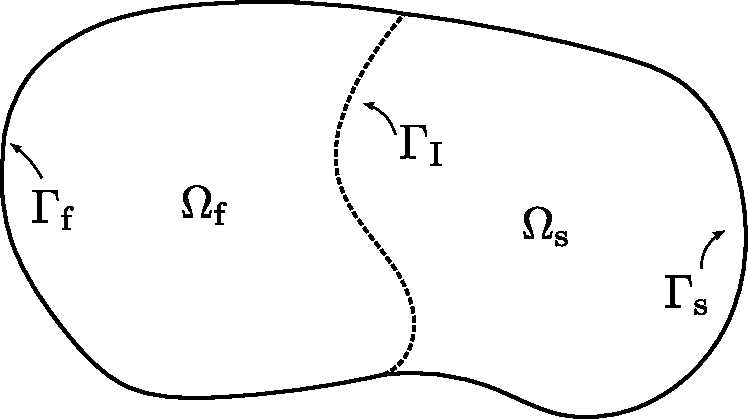
\includegraphics[scale=0.5]{Other_figures/Sketch_FSI.pdf}
 	\caption {Sketch of a general FSI problem.} 
 	\label{fig:General-sketch-fsi-problem}
 \end{figure}  

\subsection{Governing equations\label{subsec:goerning_equations_FSI}}

Using the notation introduced in the previous sections, we can extend it to account for a moving domain and incorporate the interaction between the subdomains. Therefore, the ful FSI problem can be stated as follows:
\begin{align}
 \denssolid \dudt2 - \div \lbrace \F \devPK \rbrace + \div \lbrace \psolid J \invFtrans \rbrace &= \bodyfsolid \quad && \hbox{in}~\domainsolidreference\,, t \in \timeint,  \\
 \frac{\psolid}{\kappasolid} + \dGdJ &= 0 \quad && \hbox{in}~\domainsolidreference, t \in \timeint, \\
 \devPK - 2\dWdC &= \pmb{0} \quad && \hbox{in}~\domainsolidreference\,, t \in \timeint, \\
 \usolid &= \usolidDir \quad && \hbox{on}~\boundarysolidDirichlet\,, t \in \timeint,\\
 \lbrace \F \devPK - \psolid J \invFtrans \rbrace \Normal &= \reftract \quad && \hbox{on}~\boundarysolidNeumann\,, t \in \timeint, \\
 \usolid &= \usolid^{\rm{o}} &&\hbox{in}~\domainsolidreference\,, t=0, \\
 \vsolid &= \vsolid^{\rm{o}} &&\hbox{in}~\domainsolidreference\,, t=0,\\
 \densfluid\frac{\partial \vfluid}{\partial t} + \densfluid \alevelocity \cdot \nabla \vfluid  - \nabla \cdot\sigmafluid+ \nabla \pfluid &= \bodyffluid \quad &&\hbox{in}~\domainfluid(t) , t \in \timeint, \\
    \nabla \cdot \vfluid &= 0 \quad &&\hbox{in}~\domainfluid(t) , t \in \timeint, \\
    \frac{1}{2\viscfluid}\sigmafluid-\nabla^{\rm sym}\vfluid
    &=\textbf{0} && \hbox{in}~\domainfluid(t), t \in \timeint, \\
    \vfluid&=\vfluidD  && \hbox{on} ~\boundaryfluidD(t), t \in \timeint, \\
    \nfluid \cdot \sigmafluid&=\tfluidN   && \hbox{on}~  \boundaryfluidN(t), t \in \timeint, \\
    \vfluid&= \vfluid^{\rm{o}} &&\hbox{in}~\domainfluid(0), t=0,\\
    -\lbrace \F \devPK - \psolid J \invFtrans \rbrace \NormalFSI &= \FSItractref \quad && \hbox{on}~\boundaryFSIreference, t \in \timeint, \label{eq:Solid_Interface}\\
    \vfluid&=\vboundaryFSI  && \hbox{on} ~\boundaryFSI(t), t \in \timeint .  
\end{align}

The problem described is formulated in a monolithic manner, meaning that all unknowns are solved simultaneously in a fully coupled approach. 

\begin{remark}
It is important to emphasize that in Eq. \eqref{eq:Solid_Interface}, the tractions $\FSItract$ are defined on the fluid side and act on the solid in the current configuration. These tractions are computed in an ALE framework and transferred to the solid domain, which operates in a TL framework. Therefore, they must be imposed as Neumann boundary conditions integrated over the reference configuration. To properly apply the virtual work principle within this framework, we must transform the surface integral from the current configuration to the reference one:
\begin{equation*}
    \left \langle \testusolid, \FSItract \right \rangle_{\boundaryFSI} = \left \langle \testusolid, \FSItractref \right \rangle_{\boundaryFSIreference}. 
\end{equation*}

To properly apply the virtual work principle within this framework, we must transform the surface integral from the current configuration to the reference one. The element surfaces are related by
\begin{equation}
    \normalFSI \mathrm{d}\Gamma = J \pmb{F}^{-T} \NormalFSI \mathrm{d}\Gamma^{\rm{o}} \label{eq:Nansons_formula},
\end{equation}
where $\mathrm{d}\Gamma$ denotes a surface element on the current configuration , while $\mathrm{d}\Gamma^{\rm{o}}$ denotes a surface element on the reference configuration. Taking the dot product of both sides with the current normal vector $\normalFSI$, and recalling that $\normalFSI$ is a unit vector, we obtain a scalar relation between the surface elements:
\begin{equation*}
    \mathrm{d}\Gamma = J \left \lbrace \normalFSI^T \left( \pmb{F}^{-T} \NormalFSI \right) \right \rbrace \mathrm{d}\Gamma^{\rm{o}},
\end{equation*}
and substituting this expression into the surface integral on the current configuration, we get:
\begin{equation*}
    \left \langle \testusolid, \FSItract \right \rangle_{\boundaryFSI} =  \left \langle \testusolid, J \left \lbrace \normalFSI^T \left( \pmb{F}^{-T} \NormalFSI \right) \right \rbrace \FSItract \right \rangle_{\boundaryFSIreference}   =\left \langle \testusolid, \FSItractref \right \rangle_{\boundaryFSIreference}. 
\end{equation*}

From this expression, we can find out the transformed tractions $\FSItractref$ (which act in the current configuration but are integrated over the reference surface) as:
\begin{equation*}
    \FSItractref =  J \left \lbrace \normalFSI^T \left( \pmb{F}^{-T} \NormalFSI \right) \right \rbrace \FSItract.
\end{equation*}

This definition ensures that the virtual work contributed by the fluid tractions is preserved under the transformation, allowing the solid solver to correctly interpret and apply these tractions within its TL framework. However, in a TL framework, the solid solver does not have direct access to the normal vector $\normalFSI$ in the current configuration, since all geometric quantities are defined in the reference configuration. For this reason, it is useful to return to Nanson's formula~\eqref{eq:Nansons_formula} to express $\normalFSI$ in terms of the known reference normal vector $\NormalFSI$. By normalizing both sides of Nanson's relation and taking into account that both normal vectors are unit vectors, we obtain:
\begin{equation*}
    \normalFSI = \frac{J \pmb{F}^{-T} \NormalFSI \mathrm{d}\Gamma^{\rm{o}}}{\mathrm{d}\Gamma} =  \frac{J \pmb{F}^{-T} \NormalFSI \mathrm{d}\Gamma^{\rm{o}}}{\| J \pmb{F}^{-T} \NormalFSI \mathrm{d}\Gamma^{\rm{o}} \|} = \frac{\pmb{F}^{-T} \NormalFSI }{\|\pmb{F}^{-T} \NormalFSI \|},
\end{equation*}
where $\| \cdot \|$ is the Euclidean norm. Substituting this into the expression for $\FSItractref$, we get:
\begin{equation*}
    \FSItractref =  J \left \lbrace \normalFSI^T \left( \pmb{F}^{-T} \NormalFSI \right) \right \rbrace \FSItract = J \frac{\left (\pmb{F}^{-T} \NormalFSI \right )^T \left (\pmb{F}^{-T} \NormalFSI \right )}{\|\pmb{F}^{-T} \NormalFSI \|} \FSItract =  J \frac{\|\pmb{F}^{-T} \NormalFSI \|^2}{\|\pmb{F}^{-T} \NormalFSI \|} \FSItract = J \|\pmb{F}^{-T} \NormalFSI \| \FSItract.
\end{equation*}

This final expression only involves quantities defined in the reference configuration, making it fully compatible with the TL framework used in the solid domain.
\end{remark}

\begin{remark}
If, instead of using a TL framework, one were to formulate the solid problem in an Updated Lagrangian (UL) framework, then the boundary integrals would naturally be carried out over the deformed configuration. In such a case, it would be necessary to express all relevant quantities, including stresses and normals, in terms of the current configuration. This requires transforming the PK2 stress tensor into the Cauchy stress tensor, and computing the associated tractions using the unit normal vector with respect to the deformed interface, denoted $\normalFSI$. The resulting traction vector on the interface would then be expressed as:
$$
\lbrace \frac{1}{J} \F \devPK \Ftrans - \psolid \pmb{I} \rbrace \normalFSI = \FSItract \qquad \hbox{on }~\boundaryFSI(t), t \in \timeint.
$$
This expression naturally arises in UL frameworks, where stresses and virtual work are evaluated with respect to the current configuration at each time step.
\end{remark}

\subsection{Partitioned scheme \label{subsec:iterative_scheme_FSI}}
Instead of solving the problem in its monolithic form, this work adopts a block-iterative coupling approach, where the solid and fluid mechanics problems are solved sequentially (such as it was performed in \cite{MorenoCastanarFSIVisco}).
The details of the coupling approach considered are outlined:

\begin{enumerate}
    \item We are using a \textit{strong coupling}, meaning that block-iterations are performed to ensure convergence to the monolithic problem solution. This is crucial to ensure proper interface coupling.
    \item The coupling is of \textit{Dirichlet-Neumann type}: the solid is solved using the loads provided by the fluid in each iteration, and then the fluid is computed using the interface velocities obtained from the solid.
    \item We have considered a \textit{dynamic sub-relaxation scheme} to minimize the amount of sub-iterations necessary to achieve convergence, in particular we have employed an Aitken  $\Delta^2$ relaxation scheme \cite{kuttler2008fixed}. The algorithm is initialized taking a constant relaxation parameter (usually 0.1) in the two first coupling iterations. Some works suggest relaxing the displacement field instead of the velocity field. However, based on our experience, relaxing only the velocity field ensures that the interface used by the fluid solver for traction calculations aligns perfectly with the interface displacements. Let us remark that several new techniques have been developed over the last years to improve transmission conditions, such as quasi-Newton methods \cite{FSIQN2014,FSIQN2016}, domain decomposition techniques \cite{FSIDDM2015} or weak boundary transmission conditions \cite{FSIWeak2020}, which could also be applied to the current problem.
\end{enumerate}


%Within each time step, let us denote by a superscript $k$ the $k$-th block-iteration of any variable. For clarity, let us omit the superscript with the time step counter. Suppose that from values at the $k$-th iteration, the solid is solved, obtaining the boundary velocities $\pmb{u}_{{\Gamma_{\rm i},{\textrm{s}}}}^{k+1}$. Then, the fluid is solved from the boundary velocities $\pmb{u}_{\Gamma_{\rm i}}^{k+1}$ computed as
% \begin{align*}
% \pmb{u}_{\Gamma_{\rm i}}^{k+1} = \pmb{u}_{\Gamma_{\rm i}}^{k} + \omega^{k+1} \pmb{r}_{\Gamma_{\textrm{i}}}^{k+1},
% \end{align*}
% where
% \begin{align*}
% \pmb{r}_{\Gamma_{\textrm{i}}}^{k+1} & \coloneqq \pmb{u}_{{\Gamma_{\rm i},{\textrm{s}}}}^{k+1}- \pmb{u}_{\Gamma_{\rm i}}^{k},\quad
% \omega^{k+1}  = -\omega^k \frac{(\pmb{r}_{\Gamma_{\textrm{i}}}^{k})^{T}(\pmb{r}_{\Gamma_{\textrm{i}}}^{k+1}-\pmb{r}_{\Gamma_{\textrm{i}}}^{k})}{|\pmb{r}_{\Gamma_{\textrm{i}}}^{k+1}-\pmb{r}_{\Gamma_{\textrm{i}}}^{k}|^{2}}. 
% \end{align*}

The coupling algorithm for solving the problem, based on the Dirichlet-Neumann iteration-by-subdomain approach described earlier, is presented in Algorithm~\ref{alg:algorithm1}. Problems discretized only in time are considered; the spatial approximation is done as previously described.

\begin{algorithm}
\setlist{nosep}
\footnotesize
\caption{FSI algorithm}\label{alg:algorithm1}
%\begin{itemize}
$n = 0$; loop over the number of time steps.
\begin{itemize}
\item[] $n \gets n + 1$.
\item [] $k=0$; iterate until convergence.
\begin{itemize}
 \item[] $k \gets k + 1$ (block iteration counter omitted in the following).
 \item[$\bullet$] {\bf Solve the equations for the solid}, taking into account the tractions coming from the fluid problem $\FSItractref$. At time $t^n$, omitting the superscript $n$ and the iteration counter for the unknowns, these equations are:
 \begin{align*}
    \denssolid \BDFdudt2 - \div \lbrace \F \devPK \rbrace + \div \lbrace \psolid J \invFtrans \rbrace &= \bodyfsolid \quad && \hbox{in}~\domainsolidreference, \\
     \frac{\psolid}{\kappasolid} + \dGdJ &= 0 \quad && \hbox{in}~\domainsolidreference, \\
     \devPK - 2\dWdC &= \pmb{0} \quad && \hbox{in}~\domainsolidreference, \\
     \usolid &= \usolidDir \quad && \hbox{on}~\boundarysolidDirichlet,\\
     \lbrace \F \devPK - \psolid J \invFtrans \rbrace \Normal &= \reftract \quad && \hbox{on}~\boundarysolidNeumann, \\
     - \lbrace \F \devPK - \psolid J \invFtrans \rbrace \NormalFSI &= \FSItractref \quad && \hbox{on}~\boundaryFSIreference.
 \end{align*}
 \item[$\bullet$] {\bf Compute relaxed velocities} on the interface boundary $\vboundaryFSI$ with an Aitken relaxation scheme from the solid velocities
     $\vsolid$ evaluated on the interface boundary, $ \vsolid = \frac{\delta_2 \usolid}{\delta t}\vert_{\boundaryFSI}$.
 \item[$\bullet$] {\bf Compute the domain velocity in the fluid} by solving the problem (see \cite{Mesh}):
  \begin{align*}
    -\nabla \cdot \left \lbrace \mathbb{C} \left(E_{\mathrm{dom}}\left( \pmb{x}\right),\nu_{\mathrm{dom}} \right) : \nabla^{\rm s}\vfluiddom \right \rbrace &={\bf 0} && \text{ in } \ensuremath{\Omega}_{\rm{f}}(t^n),\\
    \vfluiddom &= \vboundaryFSI  &&\text{ on } \boundaryFSI(t^n), \\
    \vfluiddom &= {\bf 0}  &&\text{ on } \Gamma_{{\rm{f}}}(t^n) \setminus \boundaryFSI(t^n),
  \end{align*}
    where $\mathbb{C}$ is the constitutive fourth order tensor in linear elasticity, $E_{\mathrm{dom}}\left( \pmb{x}\right)$ is the Young's modulus of the mesh computed at each node according to \cite{Mesh} and $\nu_{\mathrm{dom}} = 0.065$ is the Poisson coefficient of the mesh.
    \item[$\bullet$] {\bf Solve the ALE equations for the fluid}, taking into account the mesh velocity $\vfluiddom$, $\vfluidc = \vfluid - \vfluiddom$ and using the interface velocity $\vboundaryFSI$. The equations to be solved at $t^n$ are:
    \begin{align*}
 \densfluid\frac{\delta_2 \vfluid}{\delta t} + \densfluid \alevelocity \cdot \nabla \vfluid  - \nabla \cdot\sigmafluid+ \nabla \pfluid &= \bodyffluid \quad &&\hbox{in}~\domainfluid(t^n), \\
    \nabla \cdot \vfluid &= 0 \quad &&\hbox{in}~\domainfluid(t^n), \\
    \frac{1}{2\viscfluid}\sigmafluid-\nabla^{\rm sym}\vfluid
    &=\textbf{0} && \text{ in }\domainfluid(t^n), \\
    \vfluid&=\vfluidD  && \hbox{on} ~\boundaryfluidD(t^n), \\
    \nfluid \cdot \sigmafluid&=\tfluidN   && \hbox{on}~  \boundaryfluidN(t^n), \\
    %\vfluid&= \vfluid^0 &&\hbox{in}~\domainfluid(0), t=0,\\
    \vfluid&=\vboundaryFSI  && \hbox{on} ~\boundaryFSI(t^n),  
    \end{align*}
 \item[$\bullet$] {\bf Check convergence and update unknowns}. When transmission conditions are satisfied on the interface boundary up to a tolerance, the coupling iterative loop ends.
\end{itemize}
\item[] End block-iterative loop.
\end{itemize}
End loop over the number of time steps.
%\end{itemize}
\label{FSI_algorithm}
\end{algorithm}


%%%%%%%%%%%%%%%%%%%%%%%%%%%%%%%%%%%%%%%
%
% NUMERICAL RESULTS
%
%%%%%%%%%%%%%%%%%%%%%%%%%%%%%%%%%%%%%%
\section{Numerical Examples\label{sec:numerical_examples}}

% Presentación de los casos
In this section, a series of numerical examples in FSI is presented to evaluate the performance, robustness, accuracy, and applicability of the proposed stabilized mixed formulations. These examples aim to demonstrate the effectiveness of each formulation under various FSI scenarios, allowing a comprehensive comparison of their capabilities and limitations in capturing the complex dynamics of FSI problems. The first case addresses a classic problem where a fluid flows through a channel containing a flexible flap. This case reaches a steady-state solution when FSI forces are balanced. The objective is to analyze the FSI behavior for each of the formulations presented in this study. The second case examines the well-known Turek’s test \cite{turektest} to study the effects of combining different fluid and solid formulations. In this scenario, we investigate the behavior of a laminar channel flow around an elastic object, where the solution converges to an oscillatory state. The final case focuses on analyzing blood flow in a carotid artery to compare the different formulations in a realistic application in the field of computational biomechanics. Using a patient-specific geometry, this example aims to study atherosclerosis and evaluate each formulation’s effectiveness in accurately capturing complex FSI interactions in a biomedical context.

% Block-iterative scheme properties
Concerning the iterative scheme, for all examples a maximum of 10 iterations are set for both the fluid and the solid sub-problems, whose numerical relative tolerance in the $L^2$ norm is $10^{-5}$. Also, for the transmission conditions on the interface boundary (using again the $L^2$ norm), the relative tolerance is $10^{-3}$. In order to solve the monolithic system of linear equations for each sub-problem, we use the Biconjugate Gradients solver, \texttt{BiCGstab} \cite{BiconjugateGradientSolver}, which is implemented in the \texttt{PETSc} parallel solver library \cite{PETScHomePage}.

% Mesh convergence and error estimates for each subproblem
It is important to note that mesh convergence results and corresponding error estimates for both the fluid and structural domains have been addressed in previous studies. On the structural side, the $\u$ formulation discussed in Subsection \ref{subsec:u_formulation} is widely utilized, and its error analysis can be found in sources such as \cite{Bonet}. In contrast, the mixed $\up$ formulation, introduced in Subsection \ref{subsec:up_formulation}, is explored in \cite{Castanar2020}. Finally, the mixed $\ups$ formulation, detailed in Subsection \ref{subsec:ups_formulation}, is presented in \cite{Castanar2023}. For the fluid flow problem, the irreducible two-field $\vp$ formulation discussed in Subsection \ref{subsec:vp_formulation} is commonly applied, with error analysis available, for example, in \cite{blasco2001space,codina2002analysis}. Additionally, the three-field $\vpsigma$ formulation for incompressible fluids, presented in Subsection \ref{subsec:vpsigma_formulation}, is documented in \cite{castillo2014}.

% Notación 
In all numerical examples, \( s1 \) will refer to the \( \u \) formulation, \( s2 \) to the \( \up \) formulation, and \( s3 \) to the \( \ups \) formulation. For the fluid, \( f2 \) will denote the \( \vp \) formulation, while \( f3 \) will refer to the \( \vpsigma \) formulation.

%Material parameters sólidos
In the numerical examples, the material parameters for the solid will be given in terms of Young’s modulus, $\Esolid$ and Poisson’s ratio, $\nusolid$, as is commonly done in the literature. These parameters are related to the bulk modulus $\kappasolid$ and shear modulus $\musolid$ through the following expressions:
\begin{equation*}
    \musolid = \frac{\Esolid}{3(1-2\nusolid)} \quad \hbox{and} \quad \kappasolid = \frac{\Esolid}{2(1+\nusolid)}
\end{equation*}

\subsection{Flow through a channel with a flexible flap\label{subsec:flowbar}}

In this case, we investigate the interaction between a fluid and a flexible structure within a channel, a classic setup used to study FSI dynamics. A fluid flows through the channel, interacting with an elastic flap positioned in the middle, eventually reaching a steady-state solution where the forces between the fluid and the solid are balanced. The objective of this numerical example is to evaluate the formulations presented for both the solid and fluid domains and compare their performance based on the number of DOFs. Finally, the analysis also examines the volumetric locking that may occur in the solid formulations when considering a nearly incompressible flap. 

\subsubsection{Setup\label{subsubsec:flowbar_setup}}

The geometry of the problem is shown in Fig.~\ref{fig:flowbar_geometry}. The rigid channel has a height of \( H = 1 \)~m, and the flexible wall is positioned at a distance of \( 2H \) from the channel entrance. The total length of the channel is \( L = 5 \)~m. The structural bar within the channel has a width of \( l = 0.1 \)~m and a height of \( h = 0.5 \)~m.

\begin{figure*}[h]
    \centering
    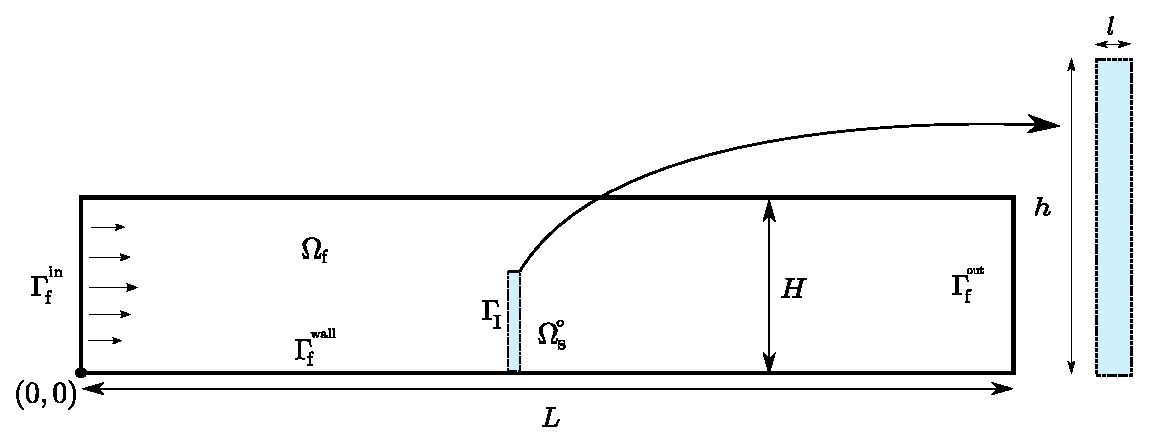
\includegraphics[width=\textwidth]{Figures_flowbar/flowbar_scheme.eps}
    \caption{Flow through a channel with a flexible flap. Geometry.}
    \label{fig:flowbar_geometry}
\end{figure*}

Regarding the properties of the fluid, the density is $\densfluid=1~\mathrm{kg}/\mathrm{m}^3$ and the dynamic viscosity is $\viscfluid=1\ \mathrm{Pa}\cdotp \mathrm{s}$.  For the elastic plate, a compressible material is assumed. The properties are as follows: an initial density $\denssolid =1~\mathrm{kg}/\mathrm{m}^3$, a Young's modulus $\Esolid=400~\mathrm{kPa}$ and a Poisson's ratio $\nusolid=0.4$. A plane strain assumption is considered.

Concerning the boundary conditions, in the inlet boundary of the fluid domain $\Gamma_{\mathrm{f}}^{\mathrm{in}}$, a steady Poiseuille flow with average velocity $\bar{\rm{v}} = 10~\mathrm{m/s}$ is assumed, given by
\begin{equation*}
    \bar{\rm{v}}_{\rm{f}}^{\rm{in}} (0,y) = 1.5 \, \bar{\rm{v}} \frac{y ( H - y )}{\left ( \frac{H}{2} \right )^2}.
\end{equation*}
On the walls $\Gamma_{\rm{f}}^{\rm{wall}}$, no-slip boundary conditions are imposed, and on the outlet $\Gamma_{\rm{f}}^{\rm{out}}$, the pressure is set to $p_{\rm{f}}^{\rm{out}}=0$~Pa. A rectangular plate is considered as the solid domain, and it is clamped at the bottom side. The considered Reynolds number is $\mathrm{Re} =\densfluid \bar{\mathrm{v}} H / \viscfluid = 10$.

We select the time step $\delta t=0.01$~s and to start the problem, a smooth increase of the inlet velocity profile in time is prescribed, given by
\begin{equation*}
    \rm{v}_{\rm{f}}^{\rm{in}} (0,y,t)=\begin{cases}
    \bar{\rm{v}}_{\rm{f}}^{\rm{in}} (0,y)\frac{1-\cos{\pi t}}{2} & \hbox{if}~t < 1.0\text{ s}\\
    \bar{\rm{v}}_{\rm{f}}^{\rm{in}} (0,y) & \text{otherwise}
    \end{cases}. \label{eq:flowbar_initial_condition_parabolic_profile_beam}
\end{equation*}

The domains are discretized by using linear structured elements (P1). Several meshes have been used for this example, whose properties are summarized in Table \ref{tab:flowbar_fluid_meshes} for the fluid domain and in Table \ref{tab:flowbar_solid_meshes} for the solid one.
\begin{table}[h]
    \centering
        \begin{tabular}{crrrrrr}
           \toprule
           \textbf{Fluid Mesh} &  \textbf{Nodes} &  \textbf{Elements} & \textbf{Element Size} & \makecell{\textbf{Element Size} \\ \textbf{FSI Boundary}} & \textbf{DOFs $f2$} & \textbf{DOFs $f3$} \\
           \midrule
           M1f & 232    & 382     & 0.2  & 0.02  & 696     & 1,392   \\
           M2f & 677    & 1,194   & 0.1  & 0.01  & 2,031   & 4,062   \\
           M3f & 2,465  & 4,622   & 0.05 & 0.005 & 7,395   & 14,790  \\
           M4f & 14,521  & 28,303  & 0.02 & 0.002 & 43,563  & 87,126  \\
           M5f & 57,141 & 112,844 & 0.01 & 0.001 & 171,423 & 342,846 \\
           \bottomrule
       \end{tabular}
    \caption{Flow through a channel with a flexible flap: Main characteristics of the fluid computational meshes.}
    \label{tab:flowbar_fluid_meshes}
\end{table}

\begin{table}[h]
    \centering
        \begin{tabular}{crrrrrr}
           \toprule
           \textbf{Solid Mesh} &  \textbf{Nodes} &  \textbf{Elements} & \textbf{Element Size} & \textbf{DOFs $s1$} & \textbf{DOFs $s2$}  & \textbf{DOFs $s3$} \\
           \midrule
           M1s & 33     & 40      & 0.05   & 66      & 99      & 198   \\
           M2s & 105    & 160     & 0.025  & 210     & 315     & 630   \\
           M3s & 561    & 1,000   & 0.01   & 1,122   & 1,683   & 3,366   \\
           M4s & 8,241  & 16,000  & 0.0025 & 16,482  & 24,723  & 49,446   \\
           M5s & 50,601 & 100,000 & 0.001  & 101,202 & 151,803 & 303,606   \\
           \bottomrule
       \end{tabular}
    \caption{Flow through a channel with a flexible flap: Main characteristics of the solid computational meshes.}
    \label{tab:flowbar_solid_meshes}
\end{table}

Before analyzing the proposed cases, Fig.~\ref{fig:flowbar_stationarysolution} shows the distribution of velocities and pressures in the channel after reaching the steady-state solution for the meshes that have already converged.

\begin{figure}[h!]
\subfloat[Velocity field]{
  \begin{centering}
    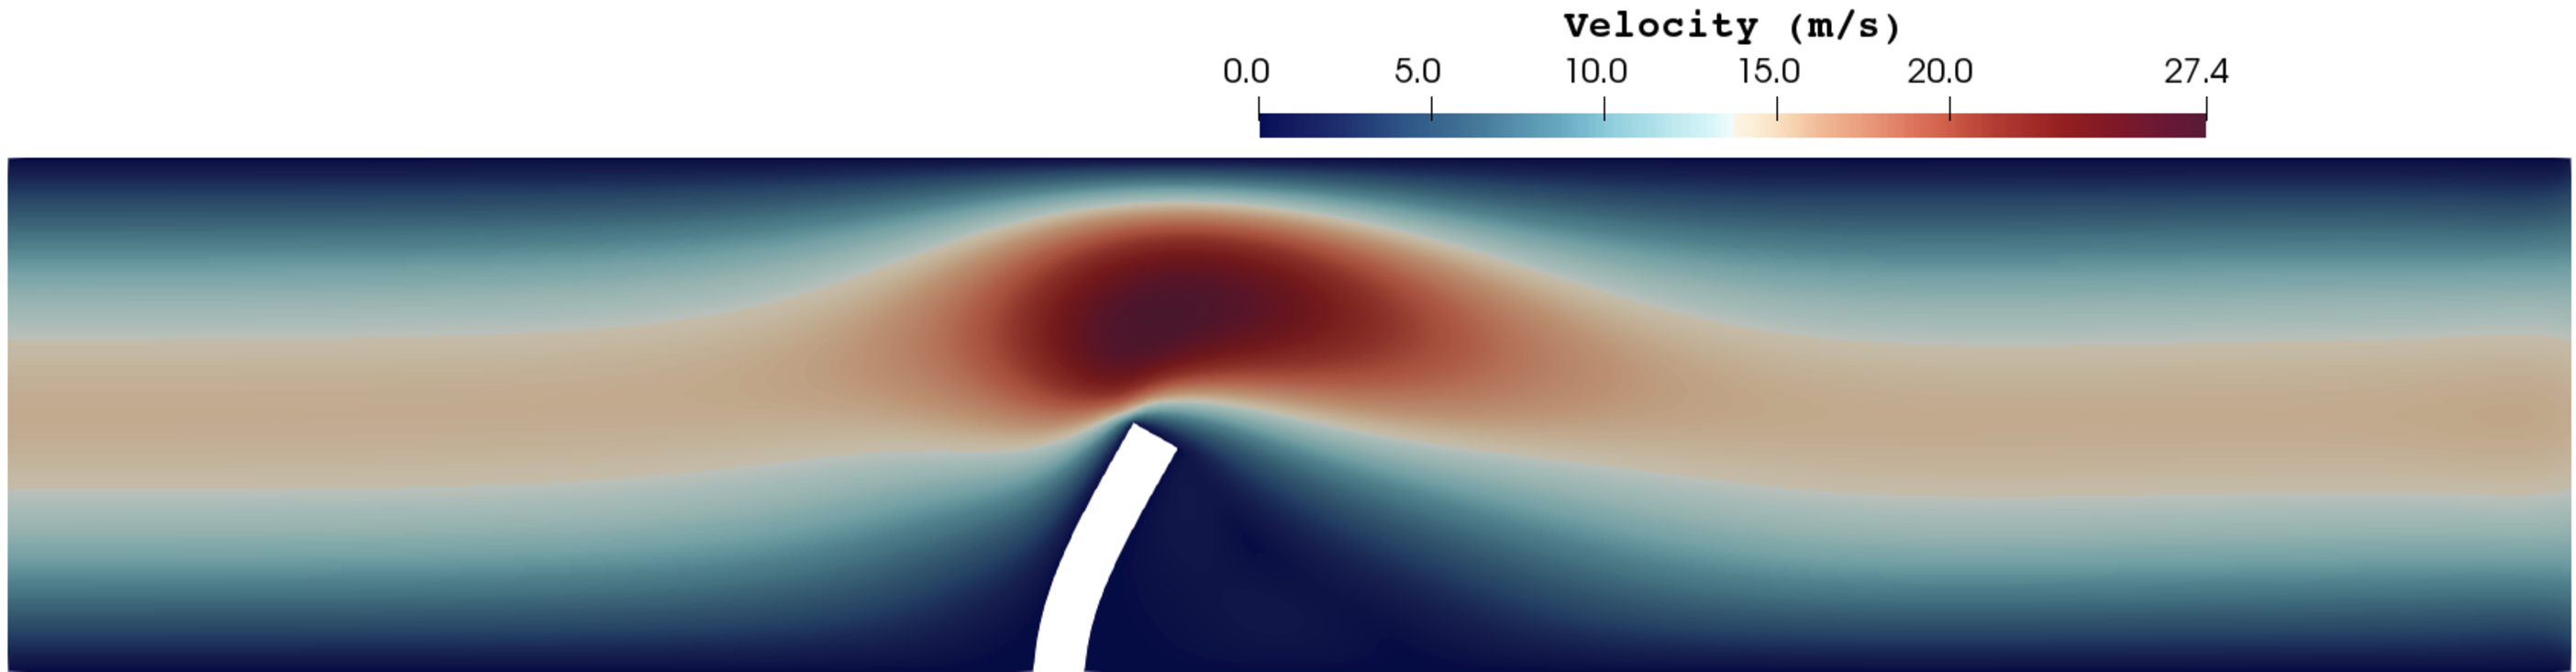
\includegraphics[width=0.99\textwidth]{Figures_flowbar/flowbar_stationarysolution_fluidvelocity.pdf}
    \par
    \end{centering}
    \label{fig:flowbar_fluidvelocity}
    }
    \\
\subfloat[Pressure field]{
  \begin{centering}
    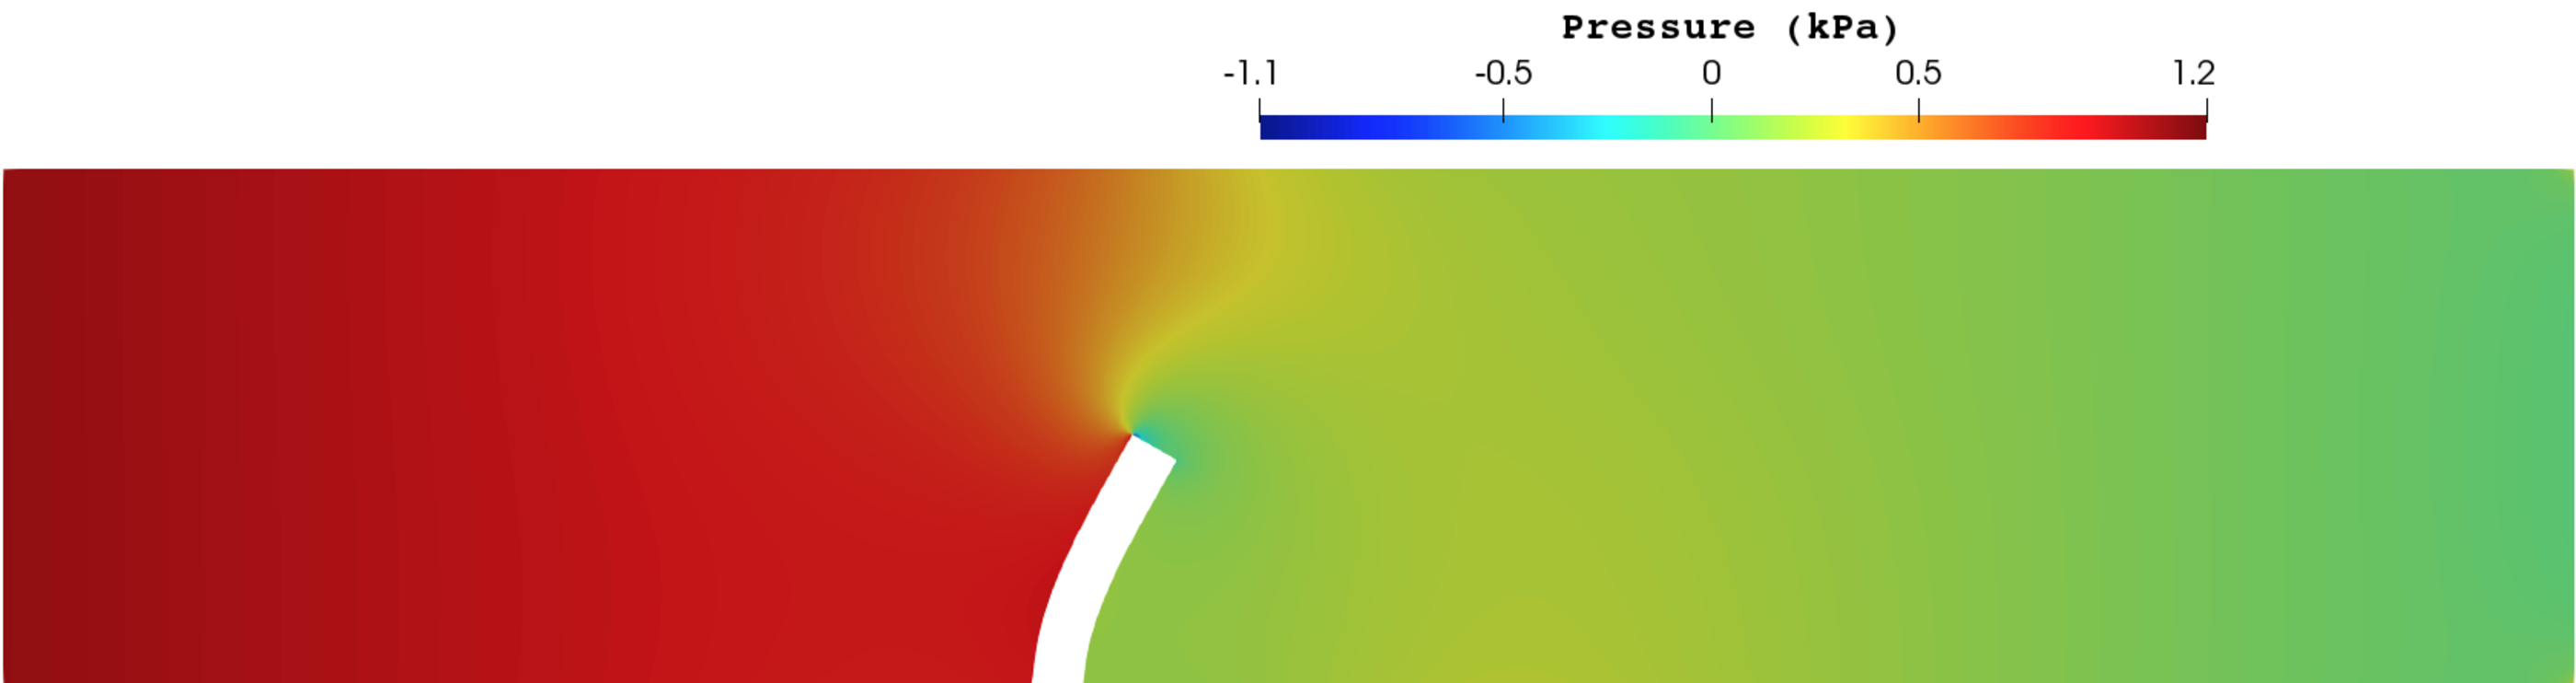
\includegraphics[width=0.99\textwidth]{Figures_flowbar/flowbar_stationarysolution_fluidpressure.pdf}
    \par
    \end{centering}
    \label{fig:flowbar_fluidpressure}
    }
   \caption{Flow through a channel with a flexible flap. Distribution of the velocity field (top) and pressure (bottom) in the fluid domain for the stationary solution. Velocities are plotted using their Euclidean norm.}
   \label{fig:flowbar_stationarysolution}
\end{figure}

\subsubsection{Solid domain formulations: a comparative study\label{subsubsec:flowbar_check_solid_formulations}}

The first study aims to analyze the impact of using each solid formulation on the overall FSI problem. To this end, we will fix a fine mesh (M4f) and use the mixed formulation f3 for the fluid, examining the different cases for all solid meshes, from M1s to M5s, across the three proposed formulations. Since formulation s1 has 2 DOFs per node, s2 has 3 DOFs per node, and s3 has 6 DOFs per node, the most appropriate comparison between formulations will be based on the number of DOFs.

\begin{figure}[h]
\subfloat[x-displacement]{
  \begin{centering}
    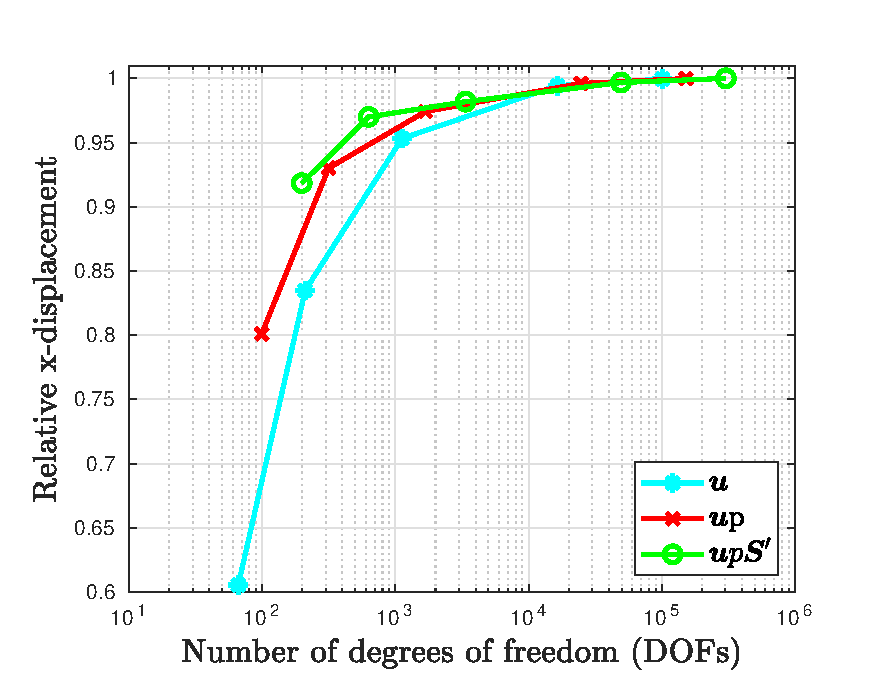
\includegraphics[scale=0.49]{Figures_flowbar/flowbar_ux_TOTAL.eps}
    \label{fg:flowbar_DOF_xdisplacement}
  \end{centering}
    }
      \subfloat[y-displacement]{
   \begin{centering}
    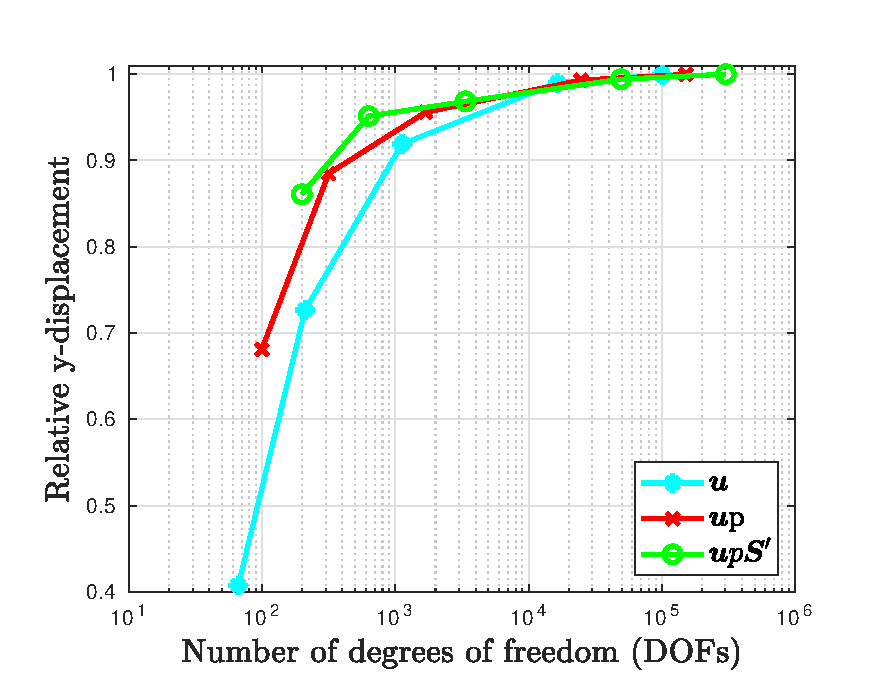
\includegraphics[scale=0.49]{Figures_flowbar/flowbar_uy_TOTAL.eps}
    \label{fg:flowbar_DOF_ydisplacement}
  \end{centering}
    } \\
    \subfloat[Drag]{
  \begin{centering}
    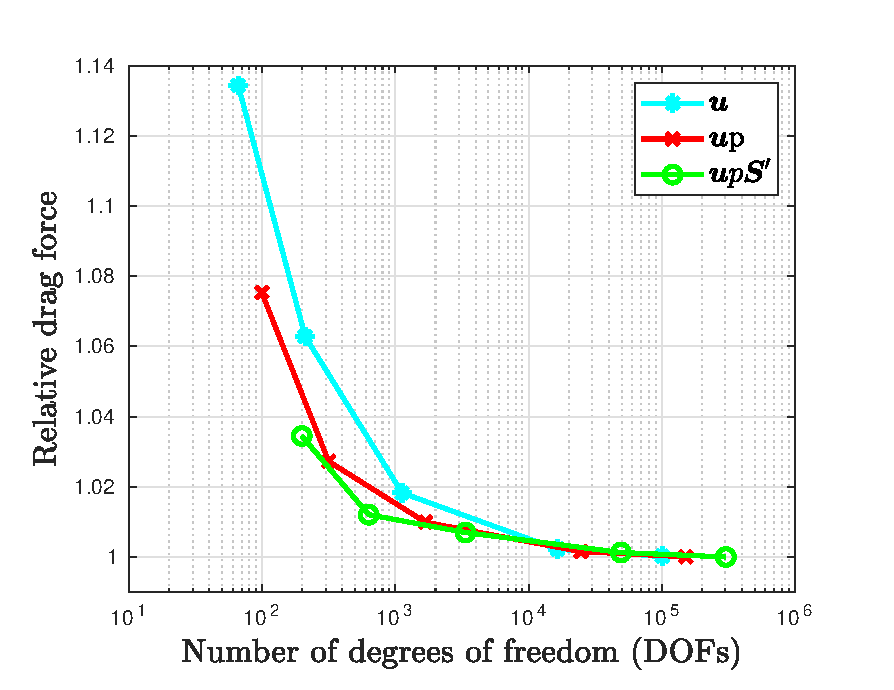
\includegraphics[scale=0.49]{Figures_flowbar/flowbar_drag_TOTAL.eps}
    \label{fg:flowbar_DOF_drag}
  \end{centering}
} 
    \subfloat[Lift]{
  \begin{centering}
    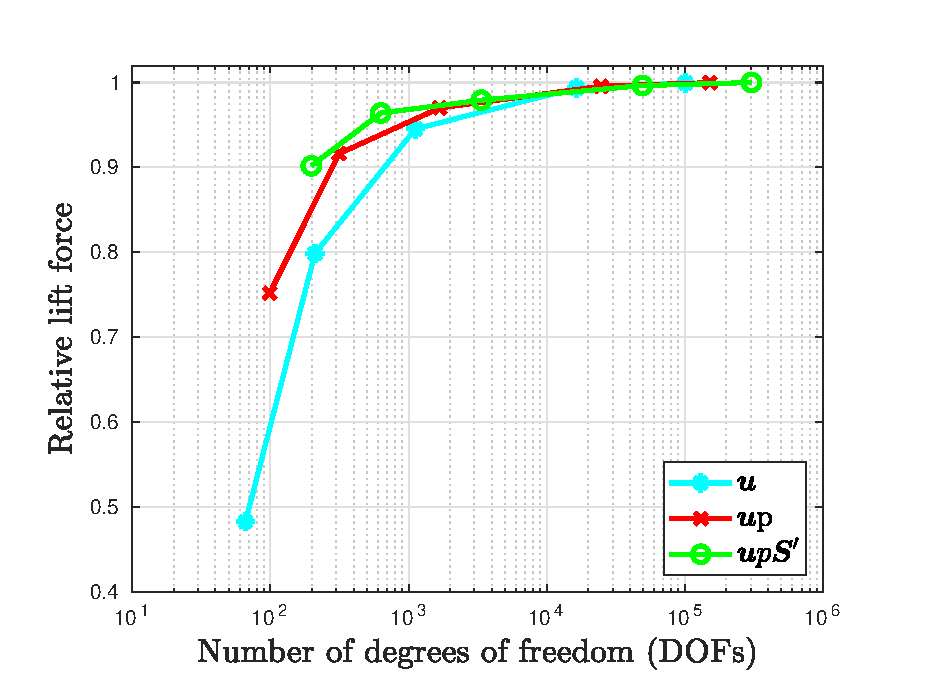
\includegraphics[scale=0.49]{Figures_flowbar/flowbar_lift_TOTAL.eps}
    \label{fg:flowbar_DOF_lift}
  \end{centering}
    } 
    \caption{Flow through a channel with a flexible flap. Comparative study for the solid formulations with respect to DOFs.}
    \label{fg:flowbar_DOF}
\end{figure}

Fig.~\ref{fg:flowbar_DOF} displays the relative convergence of the different formulations with respect to the final solution (taken as the one obtained for the s3 formulation with the M5s mesh). In this figure, we have plotted the displacements of the upper-right corner of the flap, as well as the drag and lift forces over the entire interaction surface $\boundaryFSI$. As observed in all cases, the formulation that converges the fastest is s3, followed by s2. It is also important to note that these formulations achieve higher accuracy in the variables used as unknowns (we refer the reader to \cite{Castanar2023} for more details), which is not directly reflected in these graphs. Therefore, we can conclude that using mixed formulations for the solid domain allows the final FSI solution to converge more quickly, providing good results even for coarse meshes such as M1s or M2s.

\subsubsection{Fluid domain approaches: comparative insights\label{subsubsec:flowbar_check_fluid_formulations}}

The second study focuses on evaluating the influence of different fluid formulations on the overall FSI problem. For this purpose, we fix a fine mesh (M4s) and use the mixed formulation s3 for the solid, testing various cases with all fluid meshes, from M1f to M5f, across the two proposed formulations. Since formulation f2 uses 3 DOFs per node and formulation f3 uses 6 DOFs per node, the comparison between these formulations will again be based on the number of DOFs to ensure a consistent and meaningful evaluation.

\begin{figure}[h]
\subfloat[x-displacement]{
  \begin{centering}
    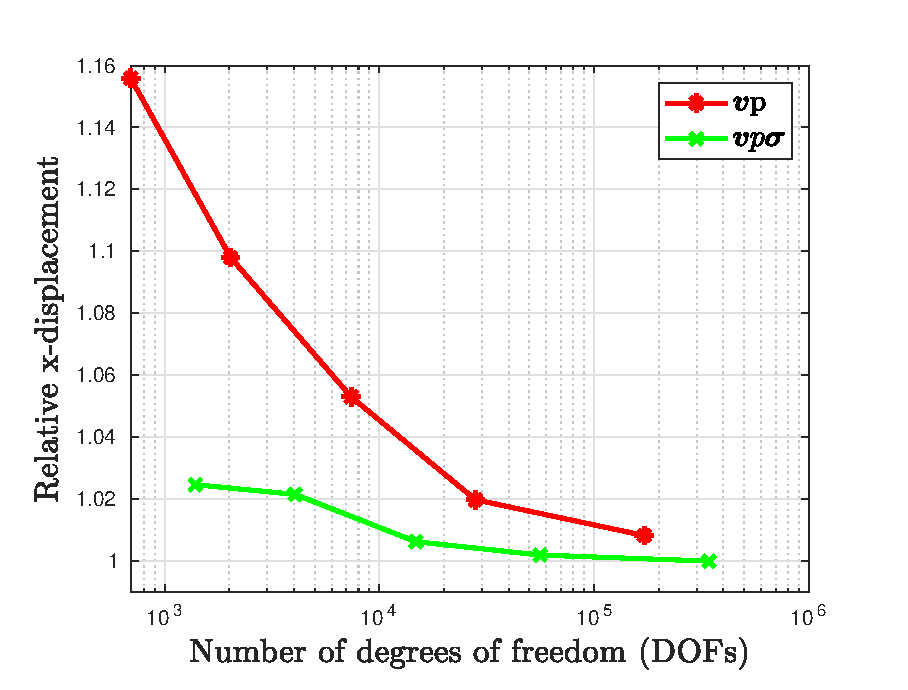
\includegraphics[scale=0.49]{Figures_flowbar/flowbar_ux_fluid.eps}
    \label{fg:flowbar_DOF_xdisplacement_fluid}
  \end{centering}
    }
      \subfloat[y-displacement]{
   \begin{centering}
    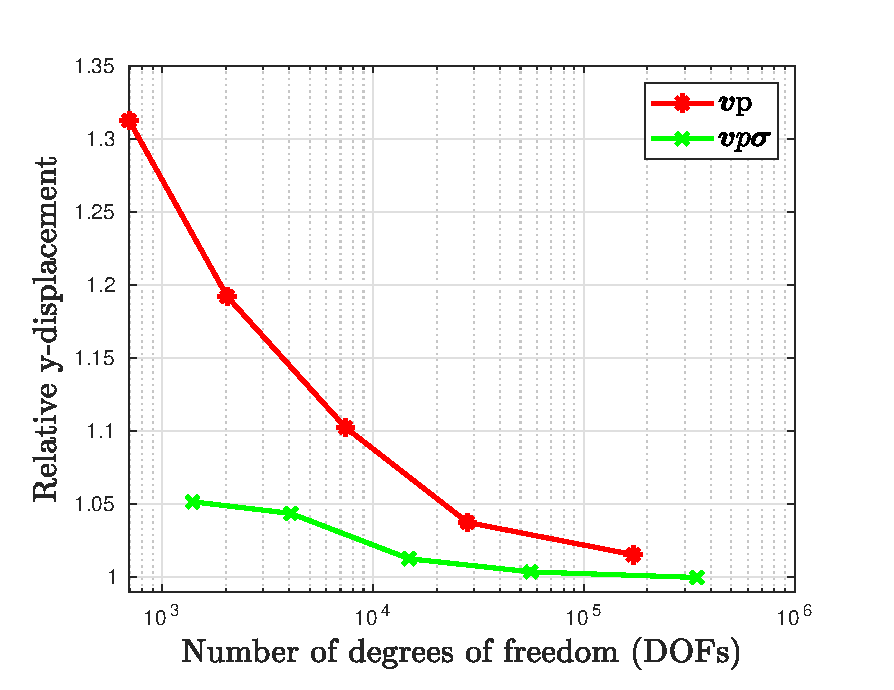
\includegraphics[scale=0.49]{Figures_flowbar/flowbar_uy_fluid.eps}
    \label{fg:flowbar_DOF_ydisplacement_fluid}
  \end{centering}
    } \\
    \subfloat[Drag]{
  \begin{centering}
    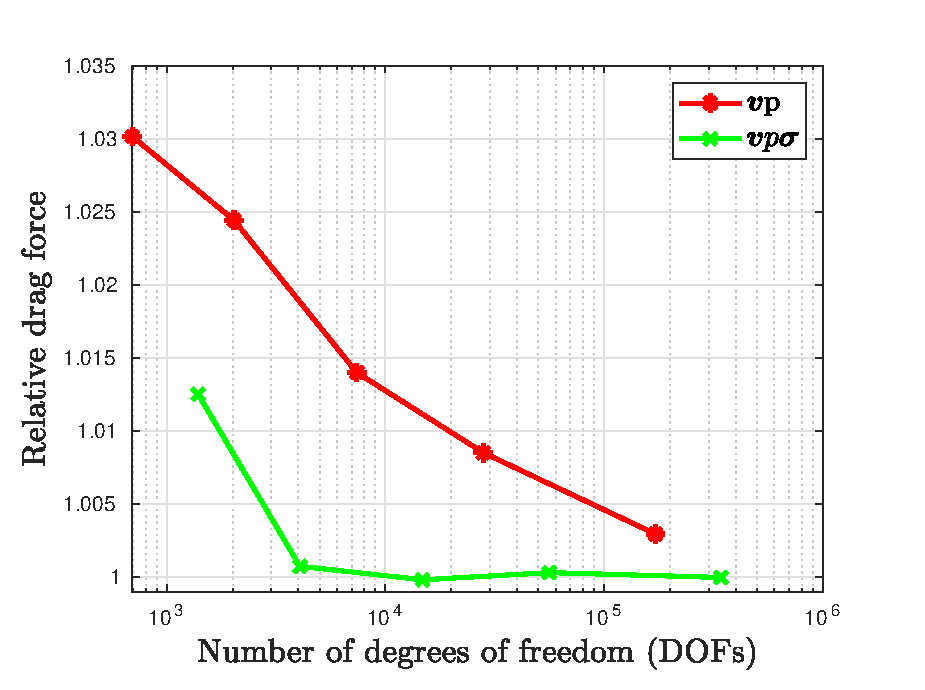
\includegraphics[scale=0.49]{Figures_flowbar/flowbar_drag_fluid.eps}
    \label{fg:flowbar_DOF_drag_fluid}
  \end{centering}
} 
    \subfloat[Lift]{
  \begin{centering}
    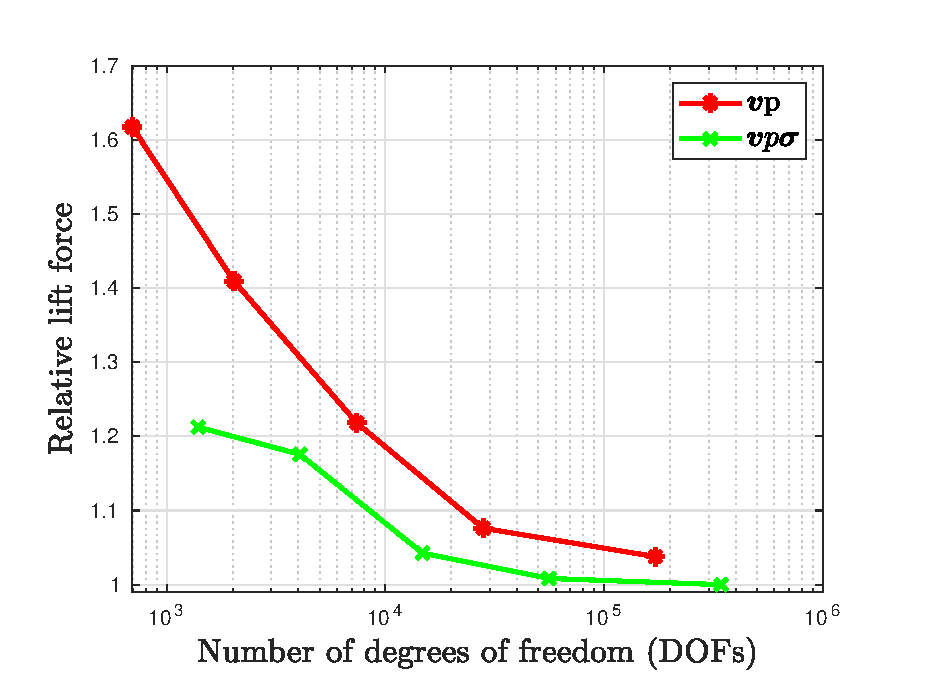
\includegraphics[scale=0.49]{Figures_flowbar/flowbar_lift_fluid.eps}
    \label{fg:flowbar_DOF_lift_fluid}
  \end{centering}
    } 
    \caption{Flow through a channel with a flexible flap. Comparative study for the fluid formulations with respect to DOFs.}
    \label{fg:flowbar_DOF_fluid}
\end{figure}

In this case, as shown in Fig.~\ref{fg:flowbar_DOF_fluid}, introducing stresses as a variable in the problem significantly accelerates the global convergence of the FSI problem compared to the irreducible formulation f2. Once again, it is demonstrated that the use of the mixed formulation f3 is highly worthwhile for addressing FSI problems effectively even for very coarse meshes.

\subsubsection{The volumetric locking. A nearly incompressible material consideration\label{subsubsec:flowbar_volumetric_locking}}

For the sake of exhaustiveness, we will now consider that the deformable bar is an elastomer or a rubber-like material. These materials exhibit the property of maintaining an almost constant volume during deformation due to their very high bulk modulus compared to their shear modulus. In such cases, Poisson’s ratio approaches $0.5$, indicating a nearly incompressible behavior. In the following simulation, we will consider a material with the same Young's modulus as before, $\Esolid=400~\mathrm{kPa}$, but a Poisson's ratio close to $0.5$, $\nusolid=0.499$. 

We conducted the same study as outlined in Subsection \ref{subsubsec:flowbar_check_solid_formulations} to analyze the evolution of the error with respect to the number of DOFs for each of the formulations presented to solve the solid dynamics subproblem. In Fig.~\ref{fg:flowbar_DOF_0499}, the displacements at the upper-right corner of the bar, as well as the drag and lift along the entire FSI boundary, are shown for the nearly incompressible material considered. As observed, the irreducible displacement formulation converges very slowly and consistently underestimates the actual solution. This phenomenon, referred to as volumetric locking \cite{Castanar2020}, occurs due to the inability of the formulation to converge to the correct solution as the material approaches the incompressible limit, leading to this type of locking. In contrast, the two mixed formulations presented in this study do not exhibit such locking, as can be clearly observed.

\begin{figure}[h]
	\subfloat[x-displacement]{
		\begin{centering}
			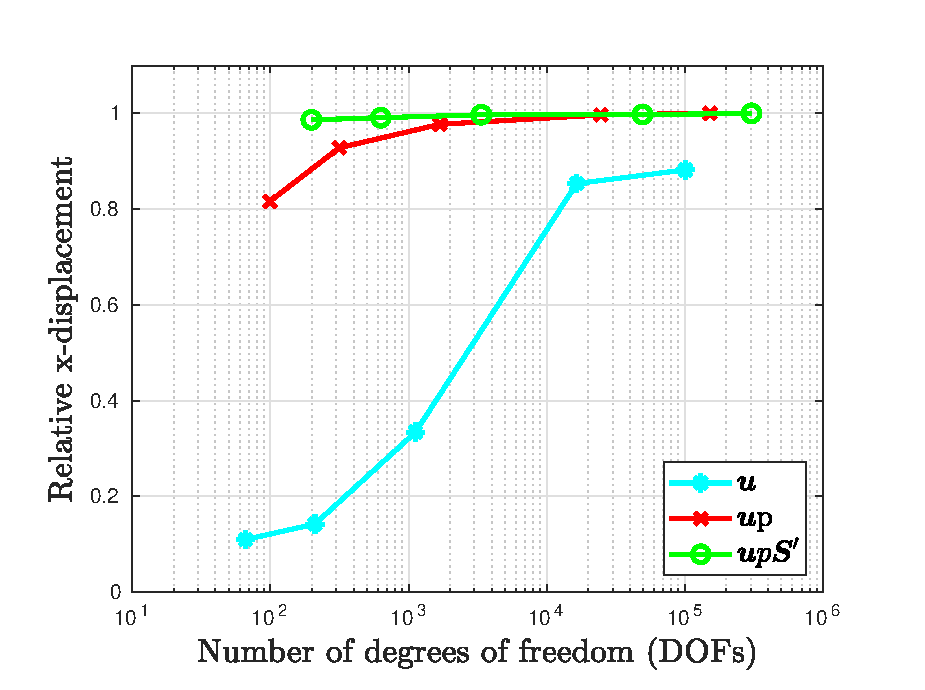
\includegraphics[scale=0.49]{Figures_flowbar/flowbar_ux_TOTAL_0499.eps}
			\label{fg:flowbar_DOF_xdisplacement_0499}
		\end{centering}
	}
	\subfloat[y-displacement]{
		\begin{centering}
			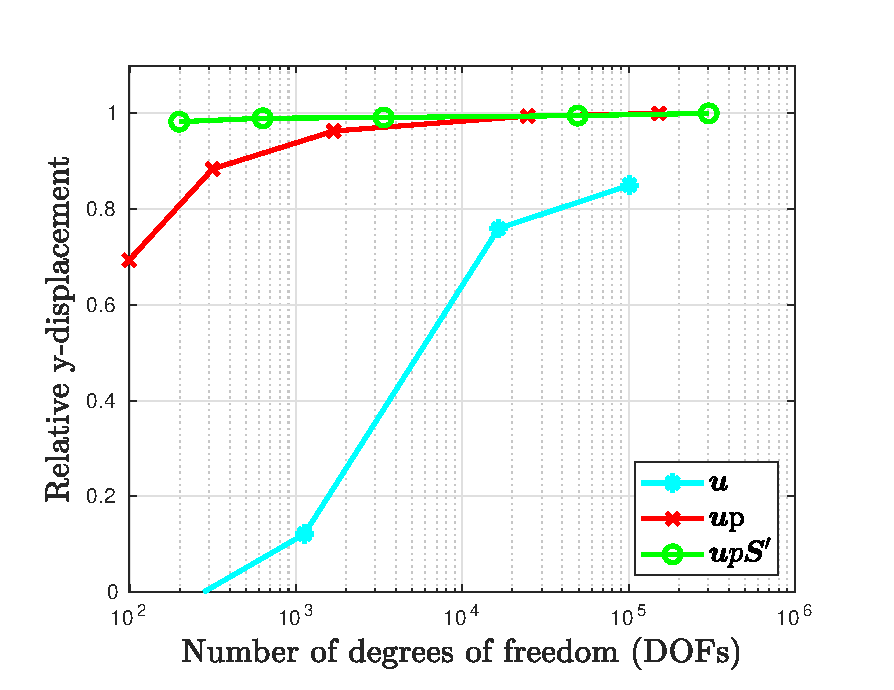
\includegraphics[scale=0.49]{Figures_flowbar/flowbar_uy_TOTAL_0499.eps}
			\label{fg:flowbar_DOF_ydisplacement_0499}
		\end{centering}
	} \\
	\subfloat[Drag]{
		\begin{centering}
			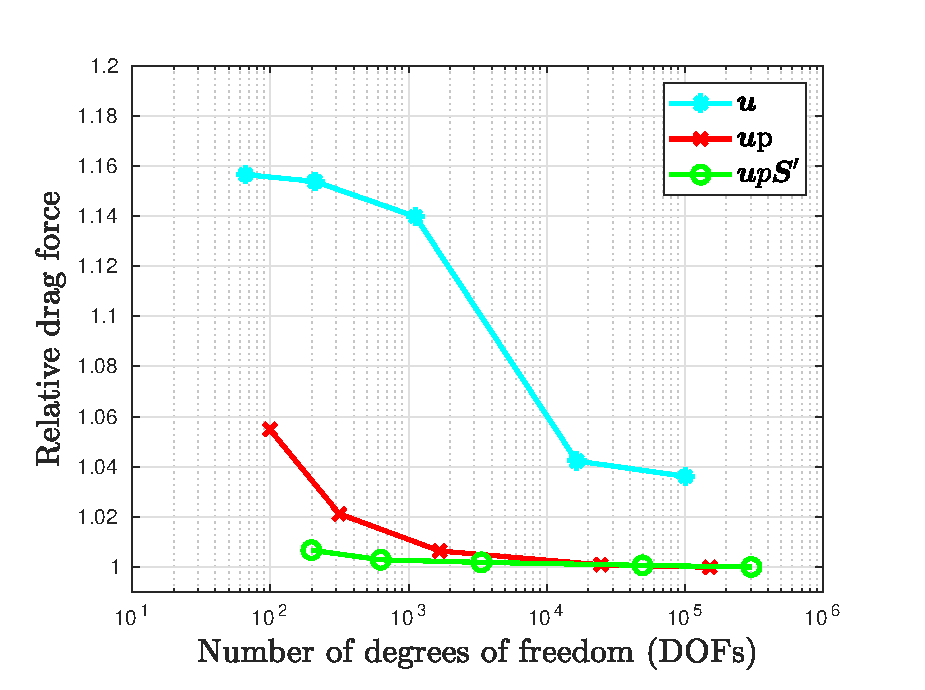
\includegraphics[scale=0.49]{Figures_flowbar/flowbar_drag_TOTAL_0499.eps}
			\label{fg:flowbar_DOF_drag_0499}
		\end{centering}
	} 
	\subfloat[Lift]{
		\begin{centering}
			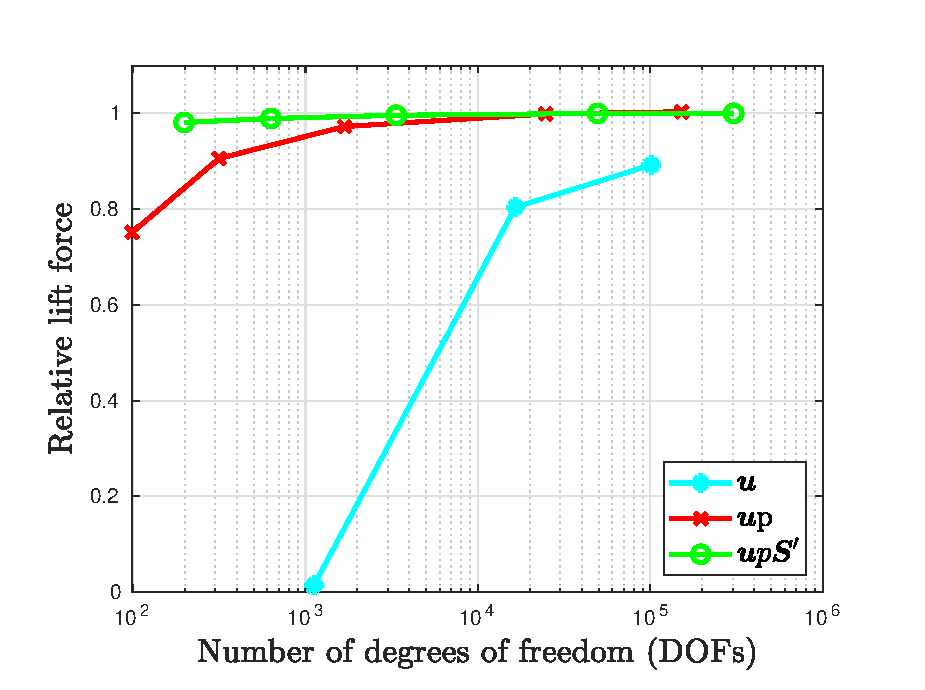
\includegraphics[scale=0.49]{Figures_flowbar/flowbar_lift_TOTAL_0499.eps}
			\label{fg:flowbar_DOF_lift_0499}
		\end{centering}
	} 
	\caption{Flow through a channel with a flexible flap. Comparative study for the solid formulations with respect to DOFs for a nearly incompressible material.}
	\label{fg:flowbar_DOF_0499}
\end{figure} 

It is important to highlight that, as expected, the locking or errors introduced in each subproblem will inevitably affect the coupled problem as a whole. For this reason, it can be observed, as anticipated, that this effect also propagates when computing the drag and lift forces exerted by the fluid on the structure.

\subsubsection{A high-Re number case. \label{subsubsec:flowbar_high_Re}}

In this subcase, we evaluate the performance of the proposed mixed formulations under more demanding flow conditions. Specifically, we reduce the fluid viscosity to $\viscfluid = 0.01 ~ \mathrm{Pa}\cdotp \mathrm{s}$ in order to achieve a Reynolds number of $\mathrm{Re}  = 1000$, using the same fluid density, characteristic velocity, and geometry as in the original configuration. High-Re conditions can introduce new challenges such as increased flow instabilities and higher-frequency content in the solution. However, it is important to emphasize that the focus of this work is not on modeling turbulence or high-Re specific stabilization, but rather on evaluating the influence of using mixed formulations within a consistent FSI coupling strategy.

\begin{figure}[h!]
    \centering
    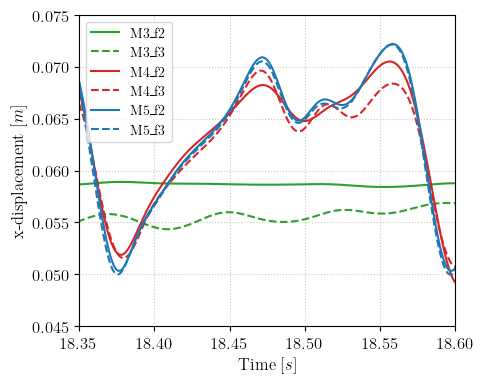
\includegraphics[width=0.45\linewidth]{Figures_flowbar/flowbar-Time-x-disp.png}
    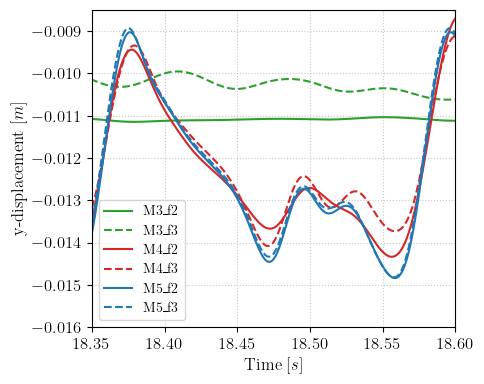
\includegraphics[width=0.445\linewidth]{Figures_flowbar/flowbar-Time-y-disp.png}\\
    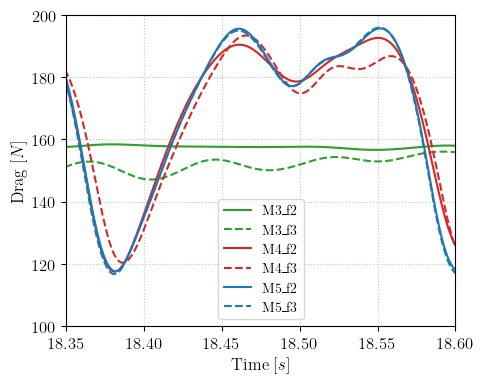
\includegraphics[width=0.45\linewidth]{Figures_flowbar/flowbar-Time-drag.png}
    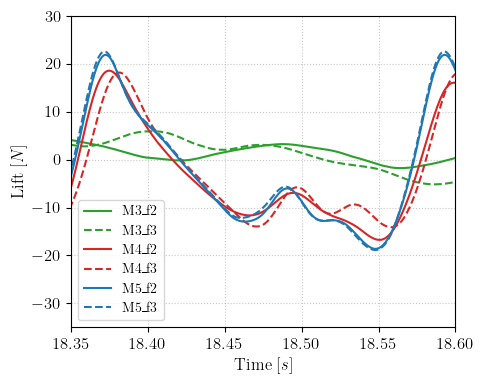
\includegraphics[width=0.45\linewidth]{Figures_flowbar/flowbar-Time-lift.png}
    \caption{Flow through a channel with a flexible flap. One period of the oscillatory solution at $\mathrm{Re} = 1000$.}
    \label{fig:flowbar_high_Re_comparison}
\end{figure}

Fig.~\ref{fig:flowbar_high_Re_comparison} shows the time evolution of the horizontal and vertical displacement at the top of the flexible bar, as well as the drag and lift coefficients, for the three finest meshes, comparing mixed formulations for the fluid side. As expected, the response becomes increasingly rich in frequencies with mesh refinement, especially in the vertical displacement and lift force. This behavior is further confirmed in Fig.~\ref{fig:flowbar_high_Re_comparison_Fourier}, which displays the frequency content of the vertical displacement signals obtained via Fourier transform.

\begin{figure}[h!]
    \centering
    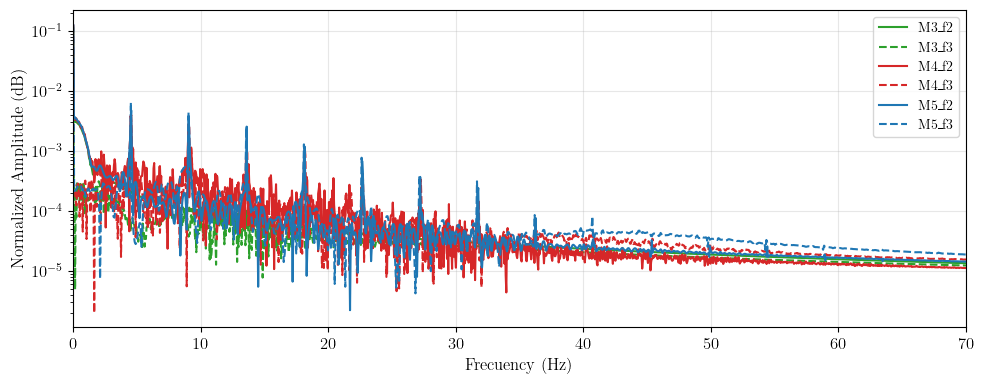
\includegraphics[width=\linewidth]{Figures_flowbar/flowbar-Fourier-transformed.png}
    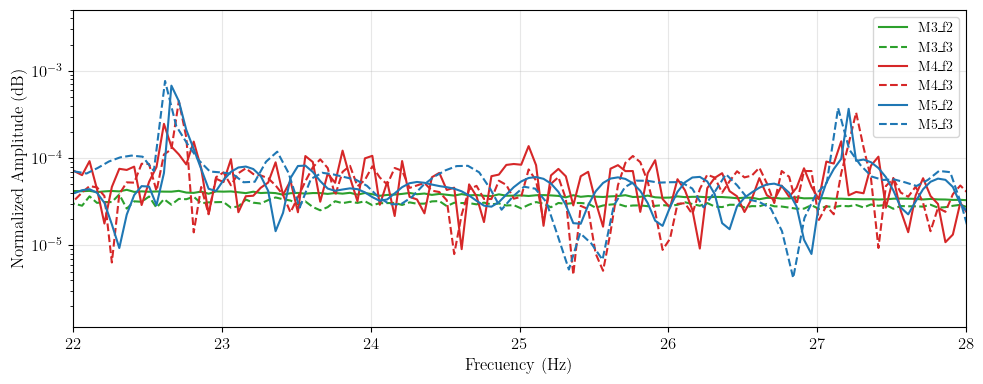
\includegraphics[width=\linewidth]{Figures_flowbar/flowbar-Fourier-transformed_zoom.png}
    \caption{Flow through a channel with a flexible flap. Fourier transform of the x-displacements at $\mathrm{Re} = 1000$.}
    \label{fig:flowbar_high_Re_comparison_Fourier}
\end{figure}

From both figures, it can be observed that the f3 formulation consistently produces smoother, more regular dynamics compared to f2. This effect is especially noticeable in the vertical motion and lift force, where spurious numerical oscillations are more effectively damped in f3. Additionally, f3 captures the dominant frequency content more accurately and robustly across meshes. These observations reinforce the idea that introducing the stress field as an independent unknown in the fluid domain leads to improved numerical behavior, even in flow regimes where inertial effects are dominant.

These results demonstrate that the advantages of the proposed mixed formulation are not limited to low-Re scenarios. The improvements in stress accuracy and numerical robustness observed in earlier examples carry over to the Re = 1000 case, confirming the method’s applicability across a broader range of flow conditions.




%-----------------------------------------------
%
% Numerical example: Turek test's
%
%-----------------------------------------------

\subsection{Turek's test\label{subsec:turek}}

In this case, we analyze the interaction between a hyperelastic structure and a laminar flow. The Turek benchmark is widely used by researchers as a reference test to validate their implementations of FSI problems \cite{turektest}. The configuration consists of a laminar channel flow interacting with a flexible structure, leading to self-induced oscillations of the solid. 
%The objective of this numerical example is to evaluate the performance of mixed formulations in a FSI problem using the Turek benchmark. Specifically, 
We compare two numerical settings: one using irreducible formulations for both domains f2s1 (s1 for the solid and f2 for the fluid) and another employing mixed three-field formulations f3s3 (s3 for the solid and f3 for the fluid). The comparison focuses on accuracy, convergence behavior, and the ability to address key numerical challenges. This study aims to demonstrate the potential advantages of mixed formulations in improving the overall FSI problem accuracy while assessing the associated computational cost.

\subsubsection{Setup}

Let us start defining the sizes of the geometry, displayed in Fig.~\ref{fig:turek_geometry}. The rigid channel measures $H = 0.41$~m in height and $L = 2.5$~m in length. The center of the circular cylinder is located at $C = (0.2, 0.2)$~m, measured from the bottom-left corner of the channel, with a radius of $r = 0.05$~m. The structural bar has a length of $l = 0.35$~m and a height of $h = 0.02$~m. Its bottom-right corner is positioned at $(0.6, 0.19)$~m, while its left end is fully attached to the fixed cylinder.
\begin{figure}[h!]
    \centering
    %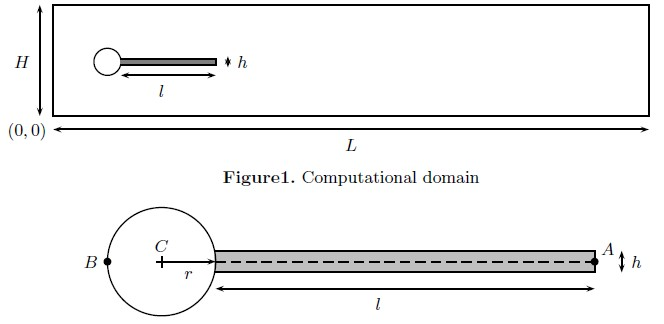
\includegraphics[scale=0.4]{Figures_Turek/turek_geometry.jpg}
    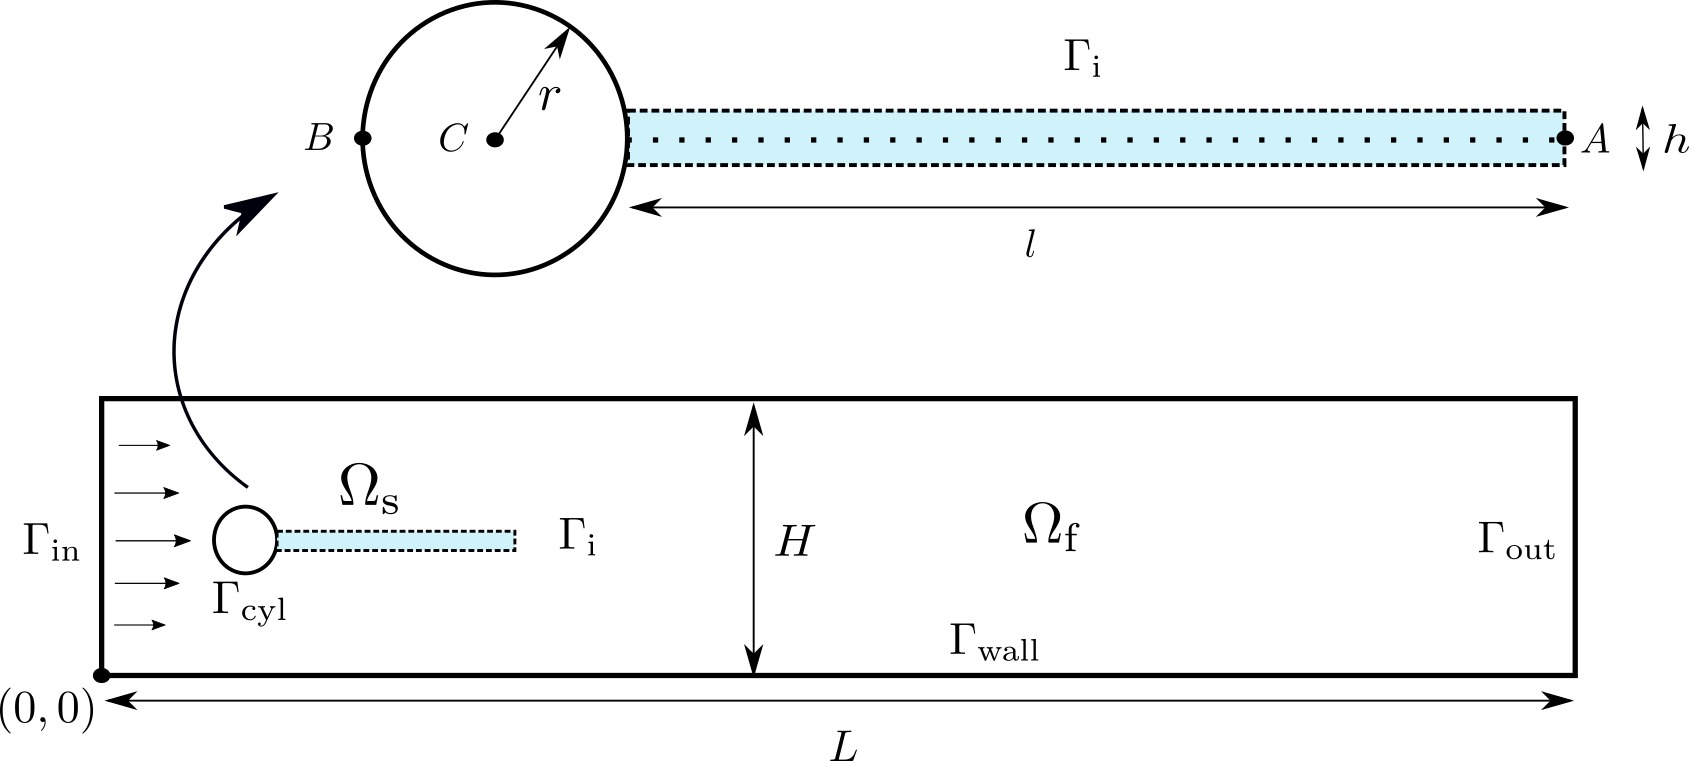
\includegraphics[scale=0.7]{Figures_Turek/Turek_scheme.png}
    \caption{Turek's test. Geometry.}
    \label{fig:turek_geometry}
\end{figure}

Let us define the boundary conditions considered for the fluid flow problem. At the channel inflow, a parabolic velocity profile is prescribed, given by  
\begin{equation}
    \bar{\rm{v}}_{\rm{f}}^{\rm{in}} (0,y) = 1.5 \, \bar{\rm{v}} \frac{y (H - y)}{\left(\frac{H}{2}\right)^2}.
\end{equation}  
Thus, the mean inflow velocity is $\bar{\rm{v}}$, and the maximum inflow velocity is $1.5 \, \bar{\rm{v}}$. Additionally, a smooth time-dependent increase in the velocity profile is considered, defined as  
\begin{equation}
    \rm{v}_{\rm{f}}^{\rm{in}}(0,y,t) = 
    \begin{cases} 
       \bar{\rm{v}}_{\rm{f}}^{\rm{in}}(0,y) \frac{1-\cos{\frac{\pi}{2}t}}{2}, & t < 2.0~\mathrm{s}, \\ 
        \bar{\rm{v}}_{\rm{f}}^{\rm{in}}(0,y), & \text{otherwise}.
    \end{cases}
    \label{eq:initial_condition_parabolic_profile}
\end{equation}  
At the outflow, a stress-free condition is applied. Additionally, a no-slip condition is imposed on the walls of the channel, as well as on the cylinder and the bar.  For the solid problem, fixed zero displacement is applied at the left edge, while all other edges are free.

Let us now define the parameter settings for the benchmark case considered. Since we aim to analyze a time-dependent problem, we select the FSI2 test detailed in \cite{turektest}, which exhibits a periodic solution. Table~\ref{fig:turek_parameter_settings} specifies the relevant parameters for both problems. Note that the fluid viscosity considered here is the dynamic one.

\begin{table}[h]
    \centering
    \begin{tabular}{l c | l c}
        \toprule
        \textbf{Parameter (solid)} & \textbf{Value} & \textbf{Parameter (fluid)} & \textbf{Value} \\
        \midrule
        $\denssolid$ {[}$\mathrm{kg/m^3}${]} & $10^4$ & $\densfluid$ ~~{[}$\mathrm{kg/m^3}${]} & $10^3$ \\
        $\Esolid$ {[}$\mathrm{MPa}${]} & 1.4 & $\viscfluid$ ~\,{[}$\mathrm{Pa}\cdot \mathrm{s}${]} & 1 \\
        $\nusolid$ ~{[}-{]} & 0.4 & $\bar{\rm{v}}$ {[}$\mathrm{m/s}${]} & 1 \\
        & & $\mathrm{Re}$ {[-]} & 100 \\
        \bottomrule
    \end{tabular}
    \caption{Turek's test. Parameter settings for Turek's test FSI2.}
    \label{fig:turek_parameter_settings}
\end{table}

%AÑADIR: Para el problema hemos usado dt bla bla , el esuqme es bdf2 ara garantizar captirar bla bla bla y se corre de 0 a 35 segundos, donde la solucion alcanza un periodicamente estacionario a partir de los 15 segundos aprox.

Finally, with respect to the domain discretization, the fluid domain is discretized using $P_1$ (linear) elements, while the solid domain is discretized with $Q_1$ (bilinear) elements. The mesh is finer around the cylinder and the bar, and becomes coarser downstream, as shown in Fig.~\ref{fig:Turek-mesh-employed}. Table \ref{tab:turek_meshes} details the three meshes employed and the corresponding DOFs for each formulation considered.
\begin{figure}[h!]
    \centering
    \subfloat[Mesh of the fluid domain]{
    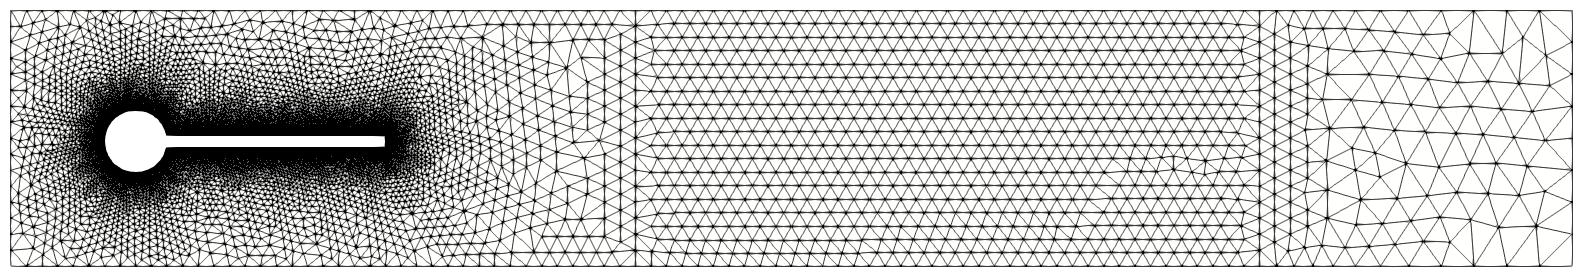
\includegraphics[scale=0.16]{Figures_Turek/Mesh_Fluid.png} \label{}}\\
    \subfloat[Zoom around the cylinder and bar and mesh of the solid domain]{
    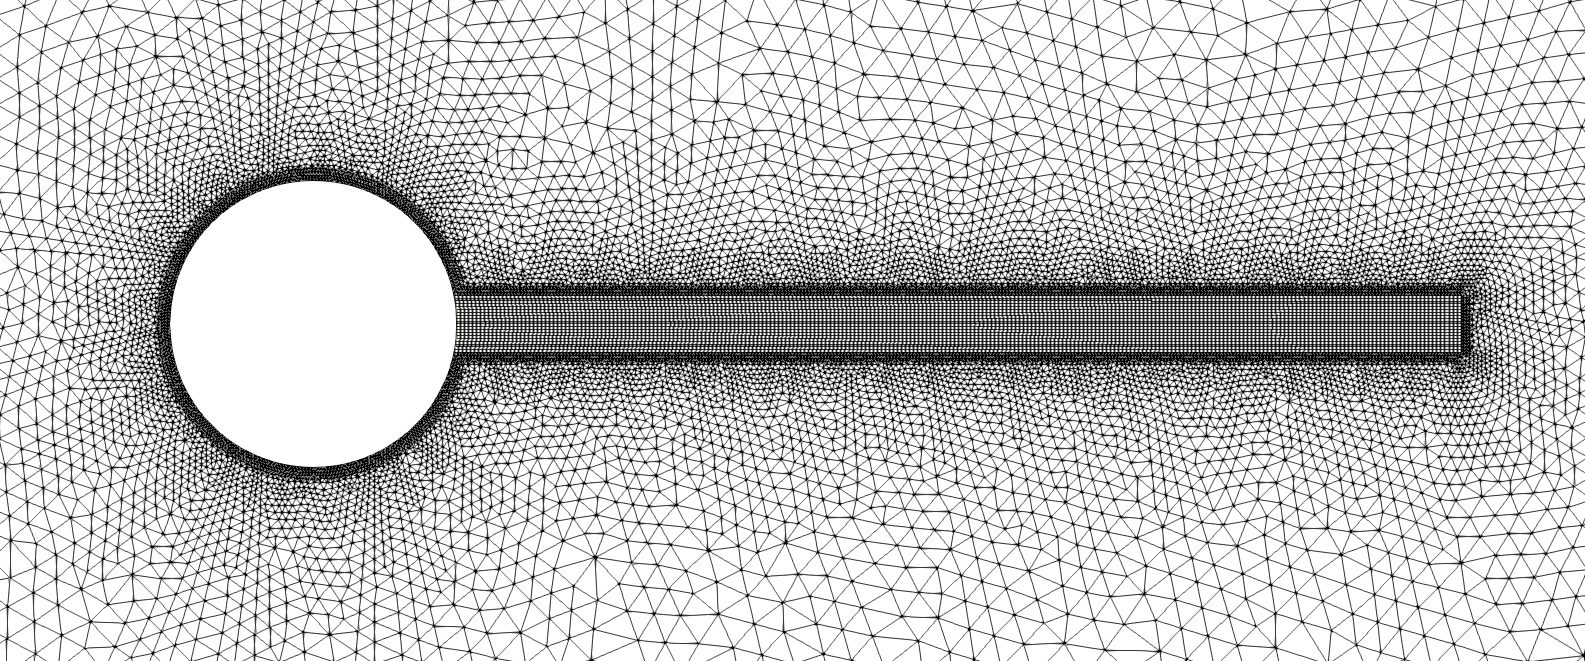
\includegraphics[scale=0.16]{Figures_Turek/Zoom_mesh.png} \label{}}
    \caption{Turek's test. FE mesh.}
    \label{fig:Turek-mesh-employed}
\end{figure}
\begin{table}[h]
    \centering
        \begin{tabular}{crrrrr}
           \toprule
           \textbf{Fluid Mesh} &  \textbf{Nodes} &  \textbf{Elements} & \makecell{\textbf{Element Size} \\ \textbf{FSI Boundary}}  & \textbf{DOFs $f2$} & \textbf{DOFs $f3$} \\
           \midrule
           M1f & 1,916  & 3,528  & 0.01  & 5,748  & 11,496   \\
           M2f & 3,105  & 5,805  & 0.005 & 9,315  & 18,630   \\
           M3f & 12,631 & 24,622 & 0.001 & 37,893 & 75,786  \\
           \bottomrule
           \toprule
           \textbf{Solid Mesh} &  \textbf{Nodes} &  \textbf{Elements} & \textbf{Element Size} & \textbf{DOFs $s1$}  & \textbf{DOFs $s3$} \\
           \midrule
           M1s & 355   & 280   & 0.005  & 710    & 2,130   \\
           M2s & 707   & 600   & 0.0035 & 1,414  & 4,242   \\
           M3s & 7,392 & 7,020 & 0.001  & 14,784 & 44,352   \\
           \bottomrule
           \bottomrule
           \toprule
           \textbf{Total Mesh} &  \textbf{Nodes} &  \textbf{Elements} & \textbf{DOFs $f2s1$}  & \textbf{DOFs $f3s3$} \\
           \midrule
           M1 & 2,271  & 3,808  & 6,458  & 13,626 \\
           M2 & 3,812  & 6,405  & 10,729 & 22,872 \\
           M3 & 20,023 & 31,642 & 52,677 & 120,138   \\
           \bottomrule
       \end{tabular}
    \caption{Turek's test. Fluid, solid and total computational meshes.}
    \label{tab:turek_meshes}
\end{table}

\subsubsection{Comparison with the Turek benchmark}

This section aims to compare our results with those from the benchmark in \cite{turektest}, using a neo-Hookean material instead of the Saint Venant-Kirchhoff solid employed in the original benchmark. The specific case considered, as introduced in the previous section, corresponds to the FSI2 configuration in the reference. The benchmark assumes a Reynolds number of 100 for the fluid flow and a slight displacement of the cylinder from the symmetry axis. These two characteristics lead to a periodic, time-dependent response of the fluid flow, inducing the motion of the beam.

Fig.~\ref{fig:Turek-different-times} presents six snapshots corresponding to three different time instants within one of the periodic cycles of the solution. The images on the left-hand side show the velocity field over the fluid domain. The results clearly demonstrate the development of vortical structures. The images on the right-hand side display the same snapshots, but with colors representing the pressure field. Note that a pressure peak is observed on the left side of the cylinder, due to the fluid flowing in the rightward direction. Additionally, the beam exhibits periodic motion, oscillating above and below its equilibrium position.

A more quantitative comparison between the results obtained in this study and those reported in the referenced benchmark can be made by analyzing the plots shown in Fig.~\ref{fig:FSI2-compaing-formulations}. In these plots, we examine four variables: the horizontal and vertical displacement of point A, located at the right end of the beam, as well as the drag and lift forces computed over both the cylinder and the beam.

Some minor differences have been observed between our solution and the one from the Turek benchmark. For instance, the frequency of oscillations is slightly higher in the reference case. Additionally, the maximum peaks in the drag force are higher in the benchmark (around 280 N), while in our study, the peak value is approximately 275 N. Despite these slight discrepancies, we consider them to be due to the different constitutive model for the solid~\cite{MorenoCastanarFSIVisco}.

%negligible. As discussed in \cite{MorenoCastanarFSIVisco}, two main factors may explain these variations. First, as previously mentioned, we use a neo-Hookean material instead of the Saint Venant-Kirchhoff solid originally considered. Second, we solve the FSI problem using a partitioned algorithm, whereas the Turek benchmark employs a monolithic approach, which may introduce some differences in the computed solution.


\begin{figure}[h!]
    \centering
    \subfloat[$t=30.0\ \rm{s}$]{
    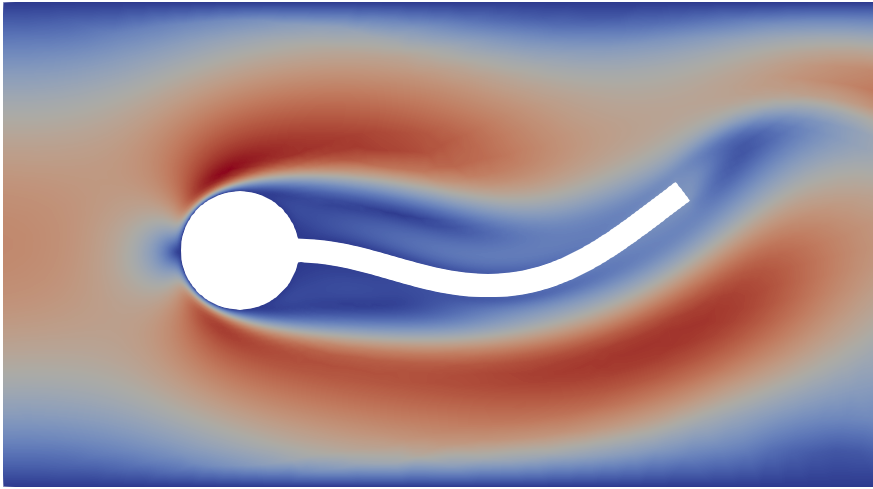
\includegraphics[scale=0.25]{Figures_Turek/t30veloc.png}  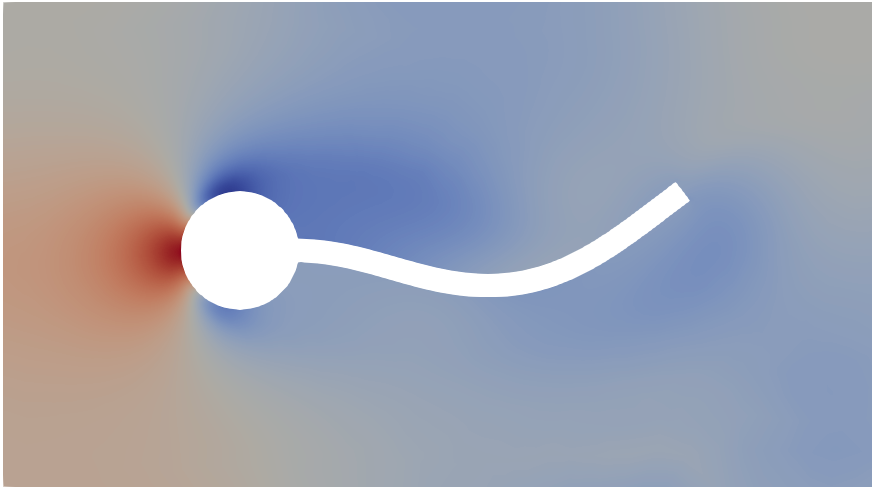
\includegraphics[scale=0.25]{Figures_Turek/t30press.png} \label{}}\\
    \subfloat[$t=32.0\ \rm{s}$]{
    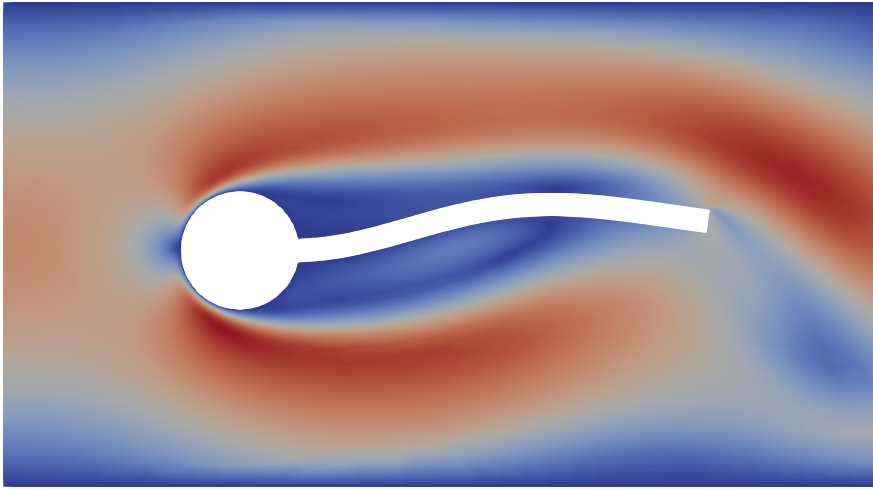
\includegraphics[scale=0.25]{Figures_Turek/t32veloc.png}  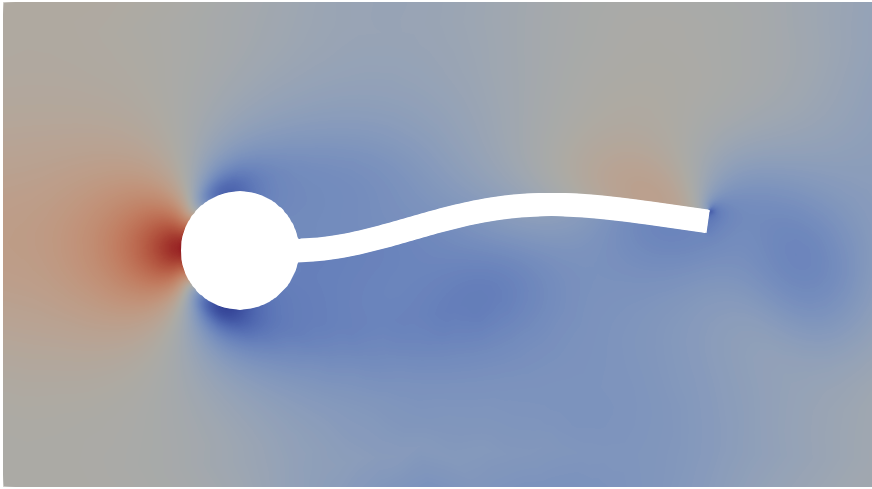
\includegraphics[scale=0.25]{Figures_Turek/t32press.png} \label{}}\\
      \subfloat[$t=33.0\ \rm{s}$]{
    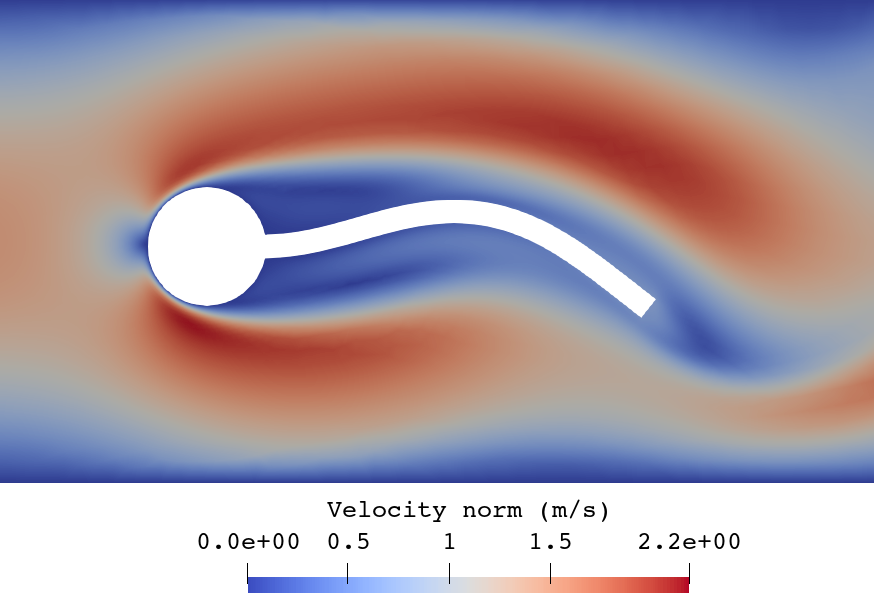
\includegraphics[scale=0.25]{Figures_Turek/t33veloc.png}  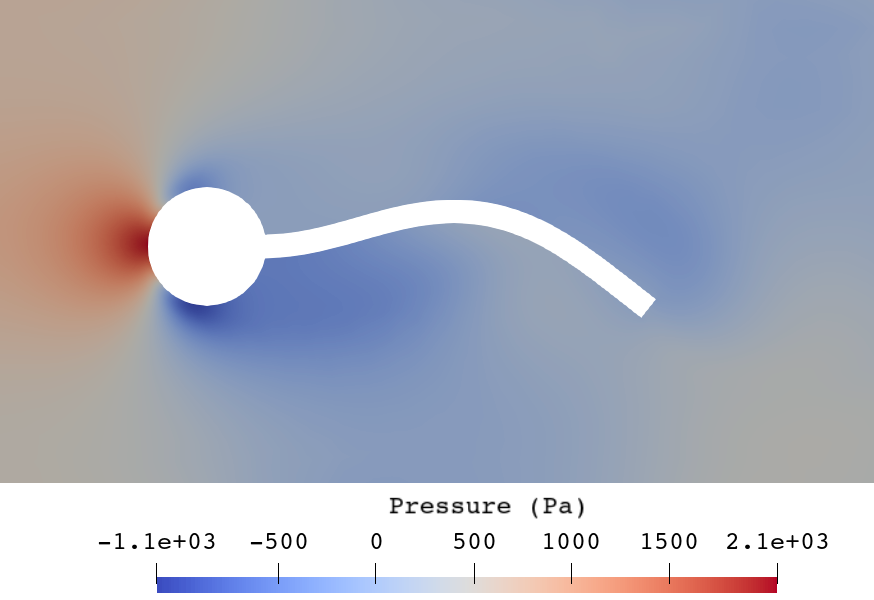
\includegraphics[scale=0.332]{Figures_Turek/t33Press_pa.png} \label{}}\\
    \caption{Turek's test. Plot of the velocity norm and pressure for test FSI2 at different time instants.}
    \label{fig:Turek-different-times}
\end{figure}


\subsubsection{Comparison between formulations}

As introduced earlier, we now seek to compare different formulations and mesh refinements. The two combinations of solid and fluid formulations considered in this study are as follows: the first involves irreducible formulations for both domains, denoted as f2s1, and the second employs mixed three-field formulations, denoted as f3s3. Details about the meshes are provided in Table \ref{tab:turek_meshes}.

We will analyze the accuracy of these two configurations by varying the mesh, considering three different refinements, which are also detailed in Table \ref{tab:turek_meshes}. In Fig.~\ref{fig:FSI2-compaing-formulations}, the following color scheme is used: green for the finer mesh (M3), orange for the medium mesh (M2), and blue for the coarser mesh (M1). Lighter colors represent the irreducible formulations (f1s1), while darker colors correspond to the mixed formulations (f3s3). It is expected that mesh refinements will yield more accurate results.

Let us first focus on the coarser mesh (blue lines). We observe a considerable improvement when the mixed formulation (lighter line) is used to model the solid and fluid domains, as compared to the irreducible formulation. However, this is not a novel result. By increasing the number of DOFs, while using the same mesh, the mixed formulation will naturally yield more accurate results.

Now, let us compare two mesh refinements, M1 and M2 (blue and orange), along with the combinations of formulations f3s3 and f2s1. While there is no noticeable difference between the drag and lift variables reported as M1\_f3s3 and M2\_f2s1, the results for the vertical and horizontal displacements of point A (located at the right end of the beam) are particularly noteworthy, as they are significantly close. This suggests that by using fewer DOFs, but with mixed formulations, we achieve a highly accurate result. This observation becomes even more apparent when we compare the case M2\_f3s3 (light orange) with the case M3\_f2s1 (dark green). It is evident that the behavior of all four measured variables is nearly identical when comparing these cases. This effect (obtaining similar accuracy with fewer DOFs) should be emphasized.

The conclusion of this study is particularly significant. It demonstrates that mixed formulations provide more accurate results, even when using coarse meshes, and with a reduced number of DOFs. This finding highlights the potential of mixed formulations applied to FSI problems to achieve accurate solutions while minimizing computational costs, which could have a high impact on the efficiency of simulations in similar contexts.

\begin{figure}[h!]
    \centering
    \subfloat[Horizontal displacement evolution at point A.]{
    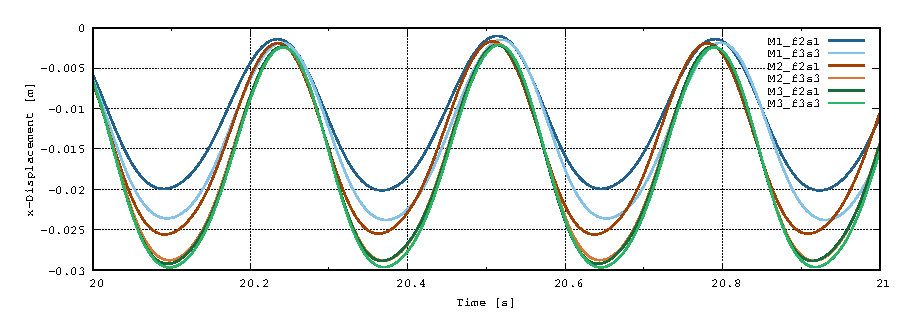
\includegraphics[scale=0.925]{Figures_Turek/x-Displacement_A.eps}}\\
    \subfloat[Vertical displacement evolution at point A.]{
    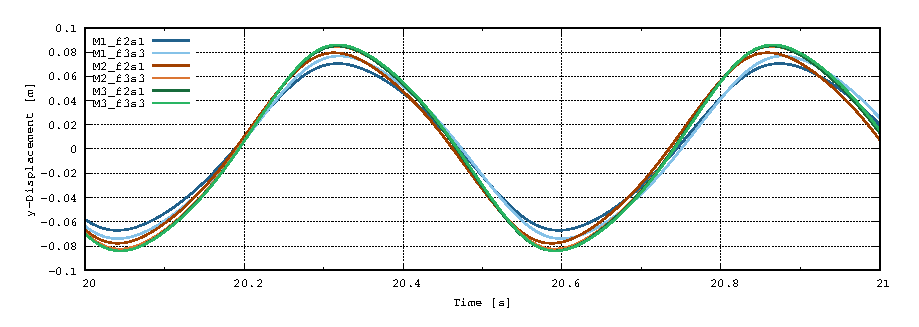
\includegraphics[scale=0.925]{Figures_Turek/y-Displacement_A.eps}}\\
    \subfloat[Lift force evolution computed around cylinder and beam.]{
    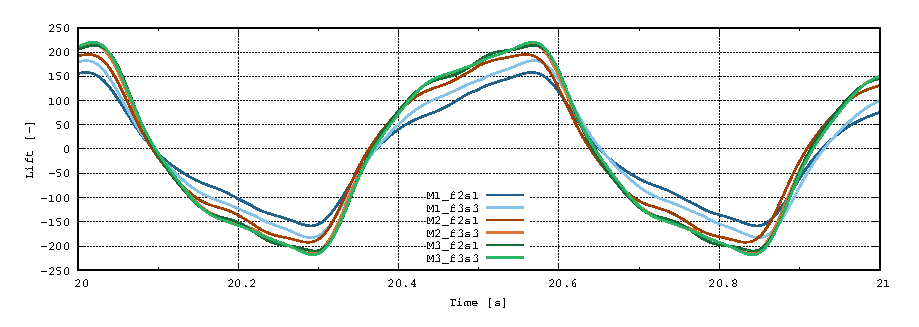
\includegraphics[scale=0.925]{Figures_Turek/Lift.eps}}\\
    \subfloat[Drag force volution computed around cylinder and beam.]{
    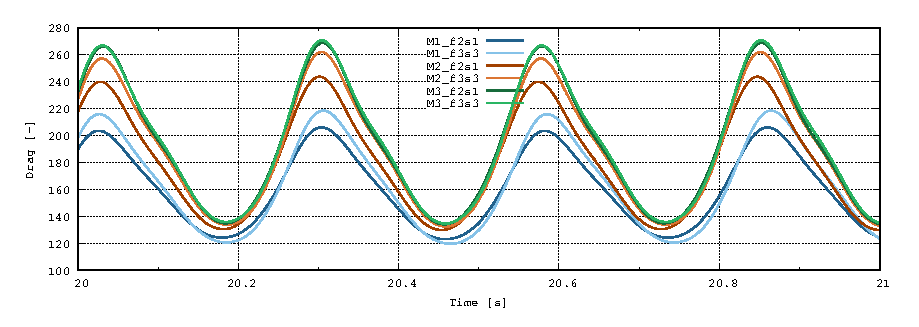
\includegraphics[scale=0.925]{Figures_Turek/Drag.eps}}
    \caption{Turek's test. Displacement at point A and drag and lift forces over the interface boundary $\boundaryFSI$.}
    \label{fig:FSI2-compaing-formulations}
\end{figure}


\subsection{Carotid blood flow\label{subsec:carotide}}

The final example presented in this work is the numerical study of blood flow in a three-dimensional carotid artery using an FSI approach. The aim is to evaluate the efficiency of mixed formulations in a relevant and applied biomechanics case.

First of all, it is important to highlight that the study of blood flow plays a crucial role in understanding the mechanisms behind the onset and progression of atherosclerosis, a precursor pathology to cardiovascular diseases such as stroke and heart attacks \cite{xu2018atherosclerosis}. 
%Numerical simulations have proven to be a powerful, cost-effective, and efficient tool for predicting blood flow behavior.
As introduced in \cite{lopes2019}, 
computational fluid dynamics techniques have been extensively used to study the hemodynamics of the carotid artery bifurcation \cite{gharabi2016,rispoli2015computational,sousa2012blood}. However, this approach has a significant limitation, as the artery's deformation directly influences the blood flow behavior. Since arterial walls are deformable, neglecting their interaction with blood flow can lead to inaccurate hemodynamic predictions, particularly in diseased arteries. With the advancement of computational power in the last decade, FSI has been increasingly applied to the study of blood flow in both healthy and stenosed vessels \cite{lee2012fluid, khader2014haemodynamics}. Despite significant progress, the effect of atherosclerosis on arterial wall mechanics is often overlooked due to the challenges in experimentally measuring vessel elasticity changes caused by the disease.

For this example, we consider the case studied by Lopes et al.~\cite{lopes2019}, where the carotid artery blood flow is analyzed to compare models with rigid and elastic walls, incorporating certain simplifications. This study has a dual objective: first, to test mixed formulations in three-dimensional problems, and second, to demonstrate that they are more computationally efficient and robust in terms of convergence compared to irreducible formulations.


\subsubsection{Setup}

Let us now define the geometry of the problem. In Fig.~\ref{fig:carotide_geometry}, we can observe the main characteristics of the chosen domain. It is important to note that the CAD model used was downloaded from the GrabCAD Library \cite{carotidCAD}, where similar computational studies have been conducted. From this CAD model, we have also generated the membrane around the carotid artery. No further simplifications have been considered.

\begin{figure}
    \centering
     \subfloat[Fluid and solid domains  \label{fig:carotide_fluid_solids_domain}]{
    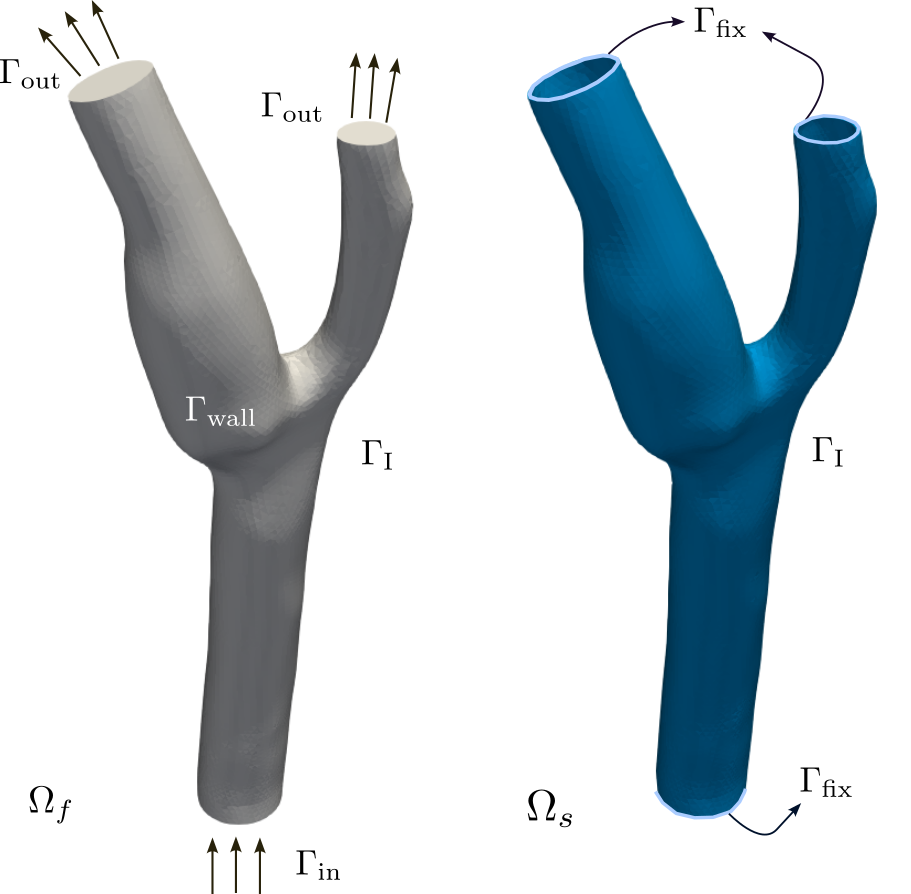
\includegraphics[width=0.55\linewidth]{Figures_carotide/carotide_geometry1.png} %0.47
    }
    \subfloat[Full domain \label{fig:carotide_fulldomain}]{
    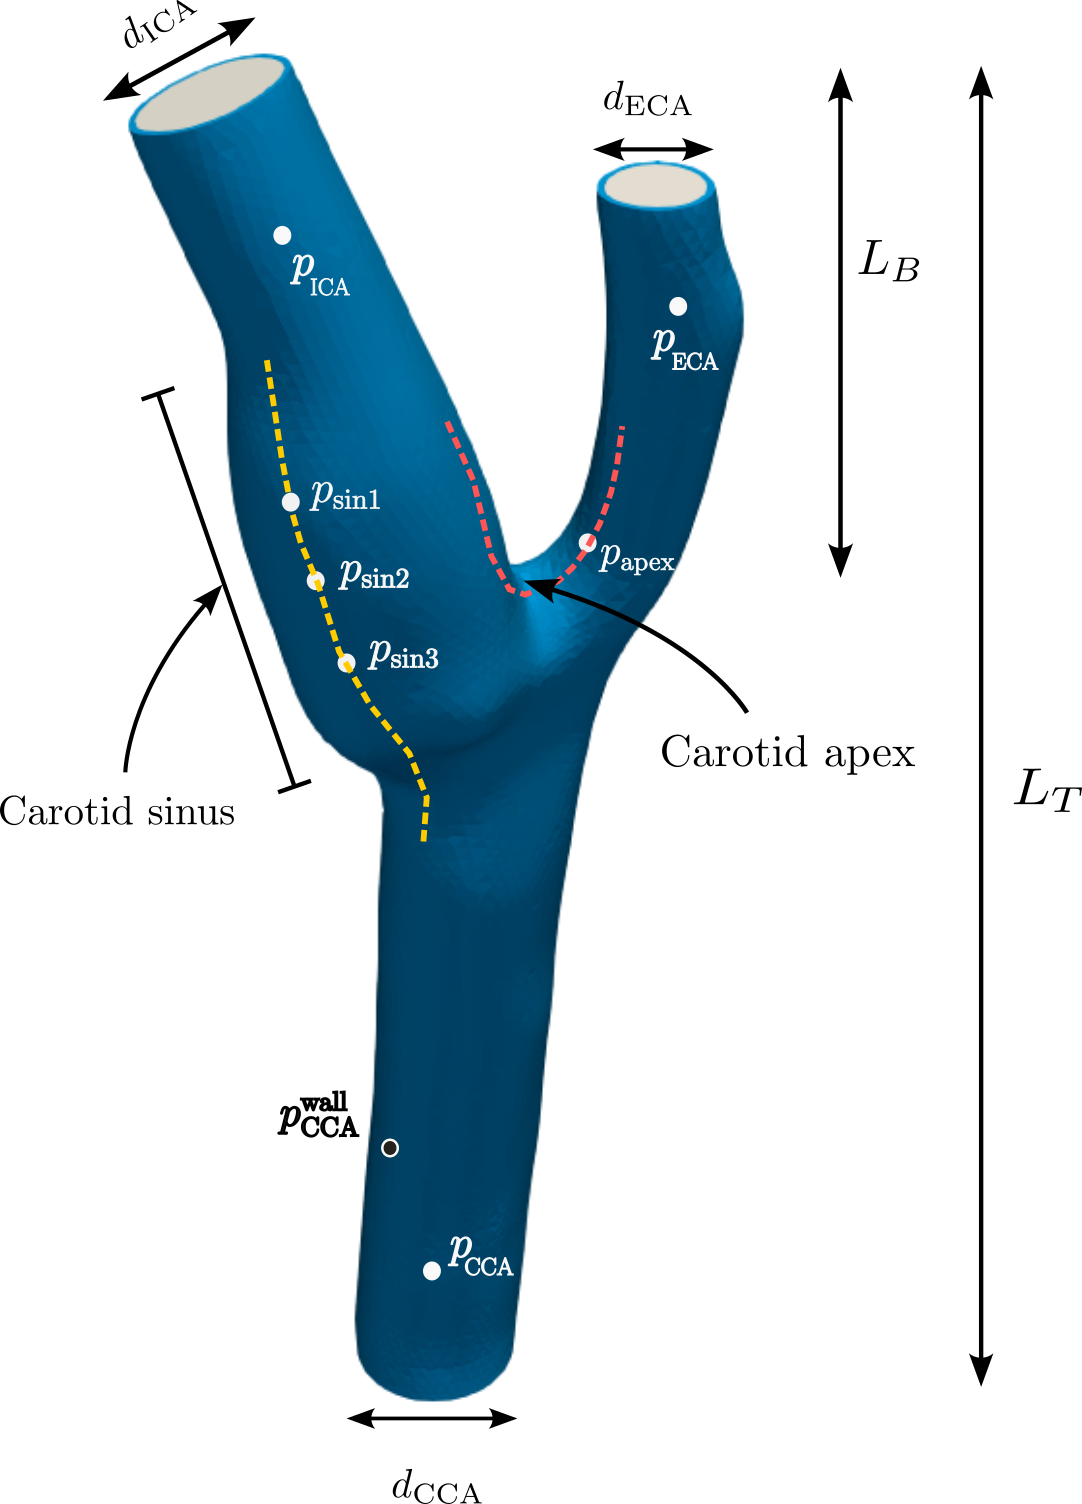
\includegraphics[width=0.38\linewidth]{Figures_carotide/carotide_setup_points.png}
    }
    \caption{Carotid blood flow. Geometry of the carotid artery bifurcation.}
    \label{fig:carotide_geometry}
\end{figure}
First, let us describe the geometric parameters detailed in Fig.~\ref{fig:carotide_fulldomain}. Upstream of the bifurcation is placed the Common Carotid Artery (CCA), which represents the inlet. Downstream of the bifurcation are located the Internal Carotid Artery (ICA) and the External Carotid Artery (ECA), which correspond to the outlets. The dilation that exists in the ICA is called the carotid sinus, or carotid bulb, and the zone of separation between the two outlet arteries is referred to as the carotid apex. The inlet and outlet diameters considered are: $d_\text{ICA} = 4.322 \ \text{mm}$, $d_\text{ECA} = 3.024 \ \text{mm}$, and $d_\text{CCA} = 6.272 \ \text{mm}$. Regarding the total length of the carotid domain, it is given by $L_T = 60 \ \text{mm}$, while the length measured from the bifurcation is $L_B = 20 \ \text{mm}$. Note that, in this case, we are working with a small-scale geometry. The membrane thickness considered is $d_m = 0.2 \ \text{mm}$.  Lastly, the yellow and red lines drawn over Fig.~\ref{fig:carotide_fulldomain} indicate the paths where some results will be presented in the next section.

Once the geometry has been described, we need to define the material properties for both the solid and the fluid. These properties are the same as those used in \cite{lopes2019}, where the fluid considered (representing blood) is Newtonian, with a density of $\densfluid = 1,060 \ \text{kg}/\text{m}^3$ and a dynamic viscosity of $\viscfluid = 3.5 \ \text{mPa} \cdot \text{s}$. For the hyperelastic solid material, we assume an initial density of $\denssolid = 1,120 \ \text{kg}/\text{m}^3$, a Poisson's ratio of $\nusolid = 0.45$, and a Young's modulus of $\Esolid = 1.106 \ \text{MPa}$.

Now, let us describe the boundary conditions considered, which are represented in Fig.~\ref{fig:carotide_fluid_solids_domain}. For the fluid domain, a no-slip boundary condition is imposed on the walls ($\Gamma_{\text{wall}}$), and a fully developed flow is assumed at the artery inlet (denoted as $\Gamma_{\text{in}}$ in the scheme). Considering the $x$ and $y$ axes contained in the inlet and $z$ normal to them, the velocity prescribed is $\vfluid = [v_x,v_y,v_z]^T$, with 
\begin{center}
    \begin{tabular}{ccc}
        $v_{x}(x,y,0,t)=0,$ & 
        $v_{y}(x,y,0,t)=0,$ & 
        $v_z(x,y,0,t)=f(t) \left(1-\dfrac{(x^2+y^2)}{r_{\textbf{CCA}}^2}\right)$  
    \end{tabular}
\par\end{center}
Note that $v_z$ is the main flow direction in the artery, $r_{\textbf{CCA}}$ is the radius of the CCA inlet, and $f(t)$ is a time-dependent function prescribing the maximum inlet velocity profile (see Fig.~\ref{fig:inlet-velocity}). Although the Womersley profile is commonly used in this type of problem \cite{hua2015influence}, we adopted a spatially parabolic profile for simplicity. \textcolor{blue}{Furthermore, three complete cardiac cycles were simulated in order to obtain a solution independent of the treatment of the initial conditions \cite{lopes2019}.}
\begin{figure}[h!]
    \centering
    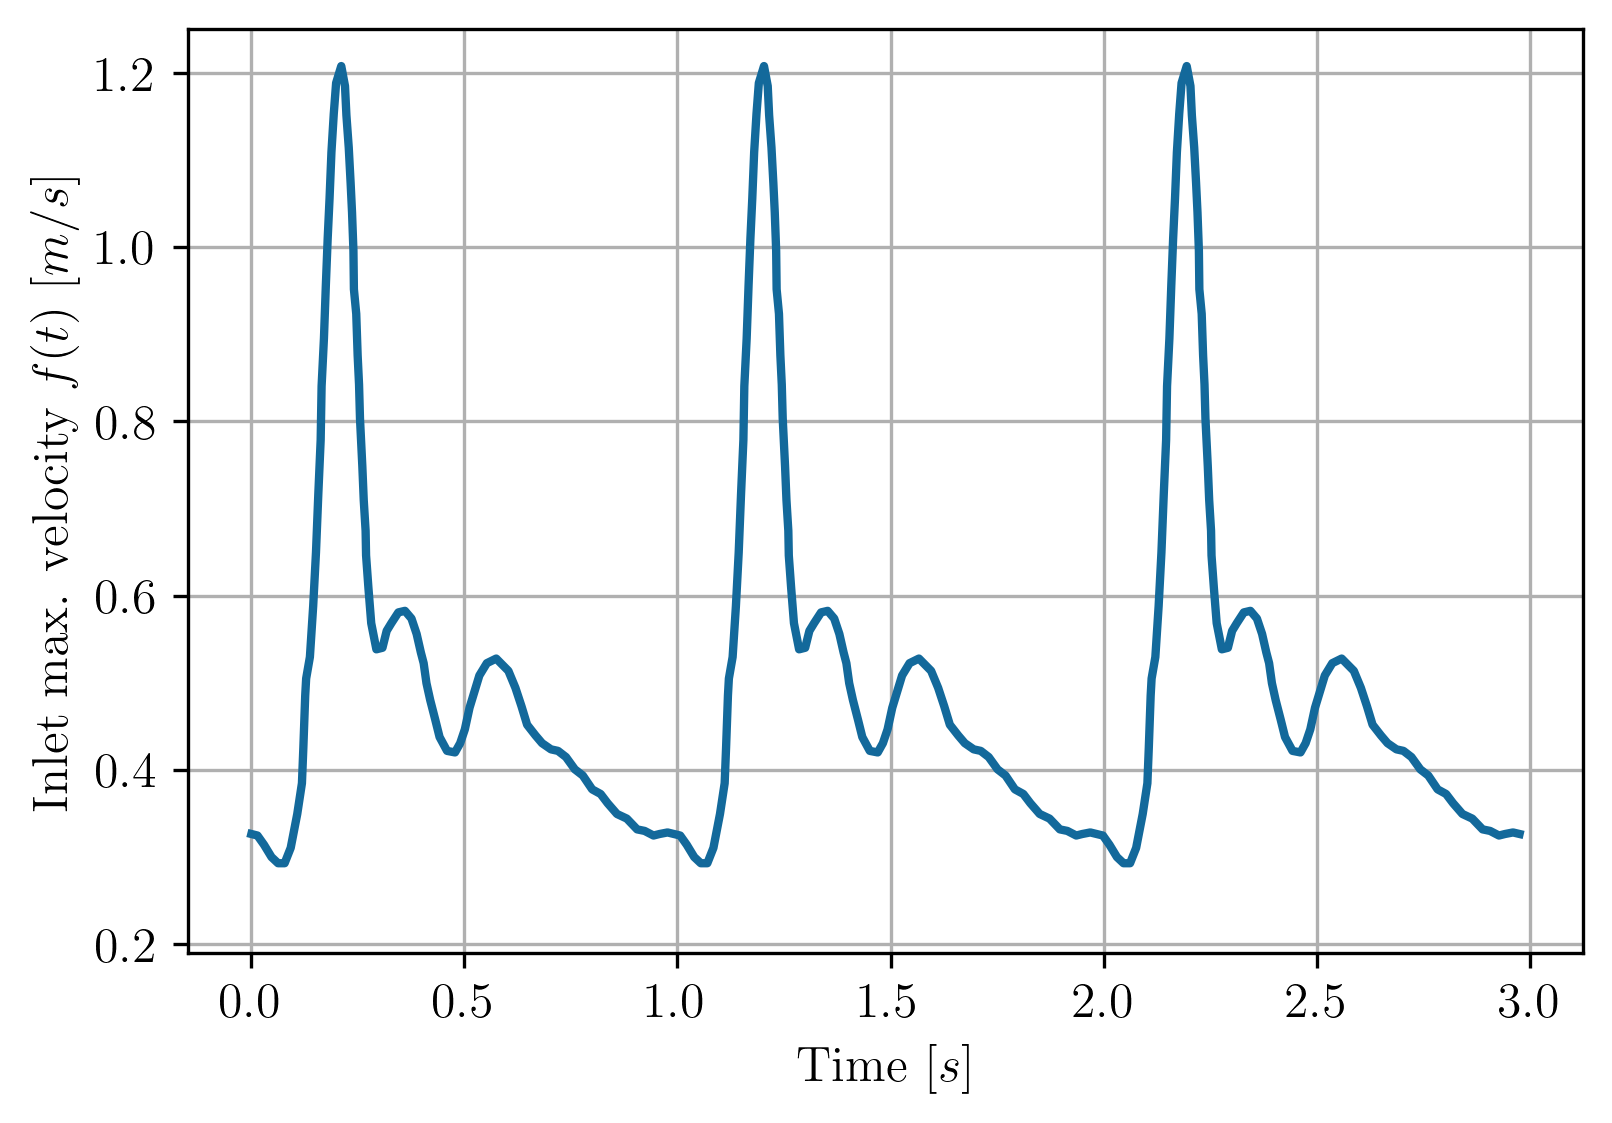
\includegraphics[width=0.6\linewidth]{Figures_carotide/Vel_max_time_plot_3cycles.png}
    \caption{Carotid blood flow. Evolution of the inlet velocity.}
    \label{fig:inlet-velocity}
\end{figure}
The outlets are denoted by $\Gamma_{\textbf{out}}$, corresponding to the outlet surfaces of the ICA and ECA arteries. In both domains, $\Gamma_{\textbf{I}}$ represents the interface domain. In the case of the fluid domain, it coincides with $\Gamma_\textbf{wall}$, which defines the surfaces that exchange information with the solid domain. Regarding the solid model, the boundaries adjacent to the inlet and outlet are fixed. On the remaining boundaries of the solid, a stress-free condition is considered, allowing the solid to deform freely in any direction.

\textcolor{blue}{Regarding the discretization, the temporal scheme used was a second-order backward differentiation formula (BDF2) scheme.}
\textcolor{blue}{In terms of spatial discretization, three different mesh refinements were considered for both the fluid and solid domains. The fluid meshes, denoted as M1f, M2f, and M3f, use a uniform element size of 0.4 mm in M1f whereas M2f and M3f incorporate local refinement along the FSI boundary with 0.2 mm and 0.1 mm elements near the wall and 0.4 mm and 0.2 mm in the interior, respectively (see Fig.~{\ref{fig:carotid-meshes}}). The solid meshes follow the same refinement: M1s has a uniform element size of 0.4 mm, M2s is refined to 0.2 mm, and M3s is refined to 0.1 mm to ensure matching resolution with the fluid along the FSI boundary. This guarantees that the evaluation of wall shear stresses is performed on a consistently refined interface.} 
The characteristics of all the meshes and formulations used in each case are detailed in Table \ref{tab:carotide_meshes}.
\begin{figure}
    \centering
    \subfloat[M1f]{
    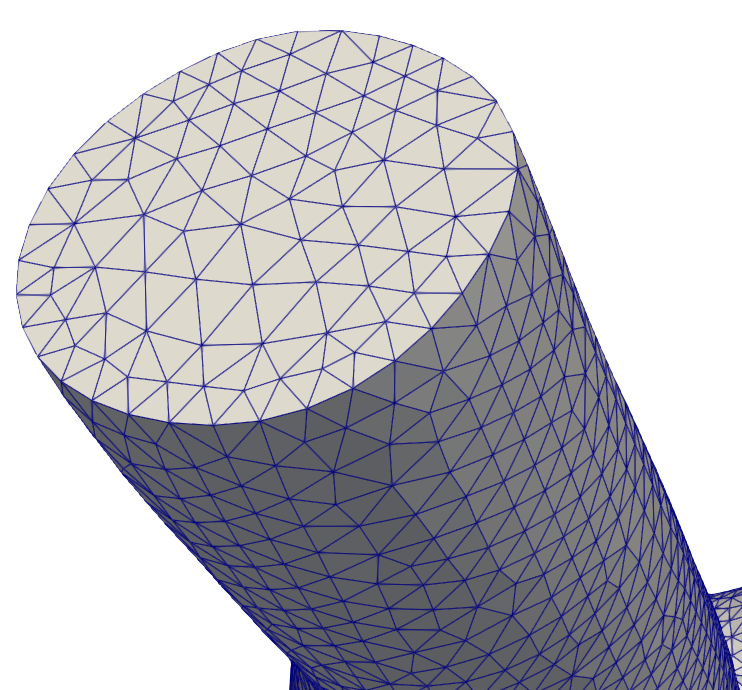
\includegraphics[width=0.275\linewidth]{Figures_carotide/Mesh1.png}}
     \subfloat[M2f]{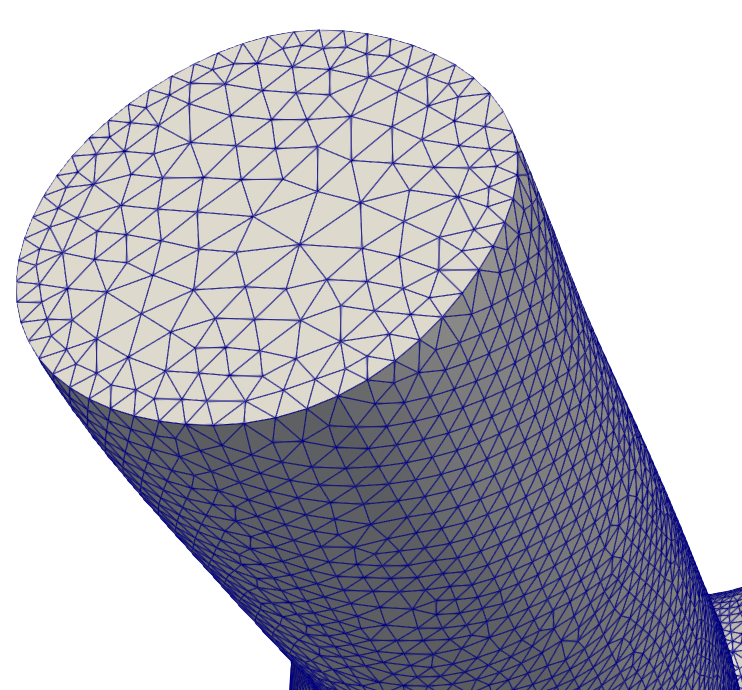
\includegraphics[width=0.275\linewidth]{Figures_carotide/Mesh2.png}}
     \subfloat[M3f]{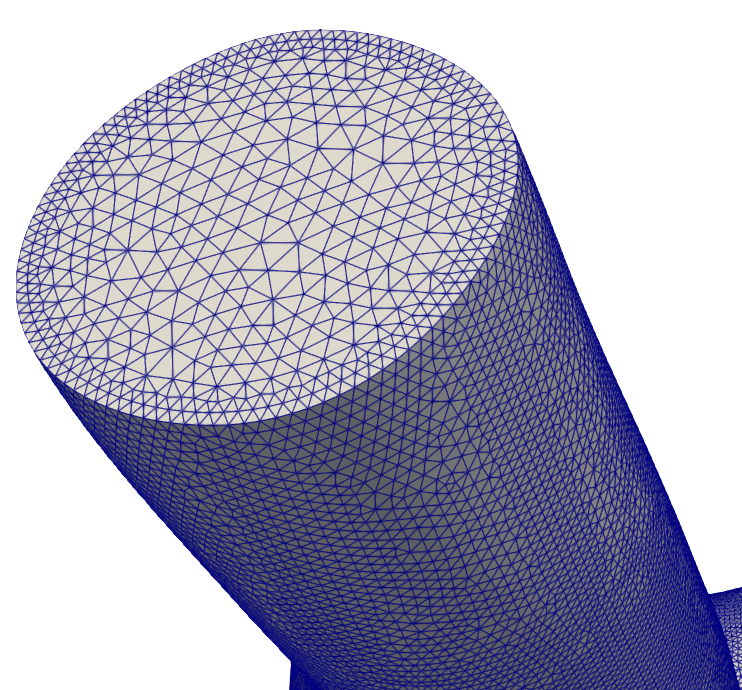
\includegraphics[width=0.275\linewidth]{Figures_carotide/Mesh3.png}}
    \caption{ Carotid blood flow. Detail of the three fluid meshes used in the simulations.}
    \label{fig:carotid-meshes}
\end{figure}
\begin{table}[h]
    \centering
        \begin{tabular}{crrrrr}
           \toprule
           \textbf{Fluid Mesh} &  \textbf{Nodes} &  \textbf{Elements} & \textbf{DOFs $f2$} & \textbf{DOFs $f3$} \\
           \midrule
           M1f & 32,413  & 163,518   & 129,652   & 324,130 \\
           M2f & 80,065  & 401,792   & 320,260   & 800,650 \\ 
           M3f & 388,425 & 2,223,321 & 1,553,700 & 3,884,250  \\
           \bottomrule
           \toprule
           \textbf{Solid Mesh} &  \textbf{Nodes} &  \textbf{Elements} & \textbf{DOFs $s1$}  & \textbf{DOFs $s3$} \\
           \midrule
           M1s & 15,885  & 47,421  & 47,655  & 158,850  \\
           M2s & 51,408  & 155,453 & 154,224 & 514,080  \\
           M3s & 154,449 & 595,657 & 463,347 & 1,544,490 \\
           \bottomrule
           \toprule
           \textbf{Total Mesh} &  \textbf{Nodes} &  \textbf{Elements} & \textbf{DOFs $f2s1$}  & \textbf{DOFs $f3s3$} \\
           \midrule
           M1 & 48,298  & 210,939 & 177,307  & 482,980 \\
           M2 & 131,473 & 557,245 & 474,484 & 1,314,730 \\
           M3 & 542,874 & 2,818,978 & 2,017,047 & 5,428,740 \\
           \bottomrule
       \end{tabular}
    \caption{Carotid blood flow. Fluid, solid and total computational meshes.}
    \label{tab:carotide_meshes}
\end{table}
%In this study, we analyze five different cases to evaluate the impact of numerical formulations on the accuracy of computations. The first two cases use the same mesh configuration, with M1f for the fluid and M1s for the solid, but employ different formulations: M1\_f2s1 follows an irreducible approach (f2 for the fluid and s1 for the solid), while M1\_f3s3 implements a three-field mixed formulation (f3 for the fluid and s3 for the solid). To further assess the advantages of the proposed mixed formulations, two more cases are introduced, M2\_f2s1 and M2\_f3s3, using a refined mesh (M2f for the fluid and M2s for the solid) while maintaining the same formulations for both subproblems. Finally, to perform a mesh convergence analysis, a fifth case is considered, M3\_f2s1 using a more refined mesh (M3f for the fluid and M3s for the solid) with the irreducible formulations for both subproblems.

Five cases are analyzed to assess the influence of numerical formulations on the solution accuracy. The first two, M1\_f2s1 and M1\_f3s3, use the same mesh (M1f–M1s) but differ in the adopted formulation: an irreducible approach (f2–s1) and a three-field mixed formulation (f3–s3), respectively. \textcolor{blue}{To further examine the benefits of the mixed formulation, two additional cases, M2\_f2s1 and M2\_f3s3, employ a refined mesh (M2f–M2s) with the same formulations. Finally, a fifth case, M3\_f2s1, uses a finer mesh (M3f–M3s) to perform a mesh convergence analysis with the irreducible formulation.}

\subsubsection{Hemodynamic parameters}

Let us now define the Wall Shear Stress (WSS), a relevant force to consider in this type of study. The WSS is the frictional force per unit area exerted by the flowing blood on the innermost layer of the arterial wall, known as the \textit{intima}. This layer is lined by the \textit{endothelium}, a thin layer of specialized cells that acts as a barrier between the blood and the vessel wall, regulating vascular function and blood flow. 
In cardiovascular biomechanics, the WSS plays a fundamental role, as the pulsatile nature of blood flow generates shear forces on the endothelium, influencing the cellular function and the pathogenesis of diseases such as atherosclerosis.
Some hemodynamic studies indicate that regions exposed to chronically low WSS are prone to atherosclerotic plaque formation due to endothelial dysfunction, increased permeability, and local inflammatory responses. Otherwise, excessively high WSS values have also been associated with plaque vulnerability \cite{malek1999hemodynamic,dolan2013high}. 

In this study we have computed this force as $\pmb{\tau_\omega}=2\viscfluid \nabla^{\text{sym}}\vfluid \cdot \nfluid$ in the case of the two-field fluid formulation and as $\pmb{\tau_\omega}=\sigmafluid \cdot \nfluid$ in the three-field formulation one. It is important to highlight that, in the two-field formulation, the WSS is computed using the velocity gradients, whereas in the three-field formulation it is directly obtained from the deviatoric part of the stress tensor, which is a nodal variable of the problem. Therefore, an increase in the accuracy of the WSS computation is expected in the latter case (not in the rate of convergence). The term "TAWSS" denotes the time-averaged WSS norm, which helps highlight regional hemodynamic differences in long-term analyses.

\subsubsection{Mesh convergence analysis}

\textcolor{blue}{To further verify the adequacy of the adopted mesh resolutions, a mesh-convergence study has been conducted for the carotid example. The objective of this study is to demonstrate that the intermediate mesh M2 is sufficiently refined, particularly in the near-wall region, to capture the relevant flow features and WSS distributions.} \textcolor{blue}{Fig.~\ref{fig:placeholder} shows that the results obtained with M2 and M3 are virtually identical for both the velocity and the pressure fields. The differences in peak velocity and pressure magnitudes are practically indistinguishable, confirming that M2 already provides mesh-independent results at the wall. These results validate the adequacy of M2 for the comparative analysis between formulations, and confirm that the refinement introduced along the FSI boundary is sufficient to capture the near-wall behavior of the flow.}

\begin{figure}
    \centering
    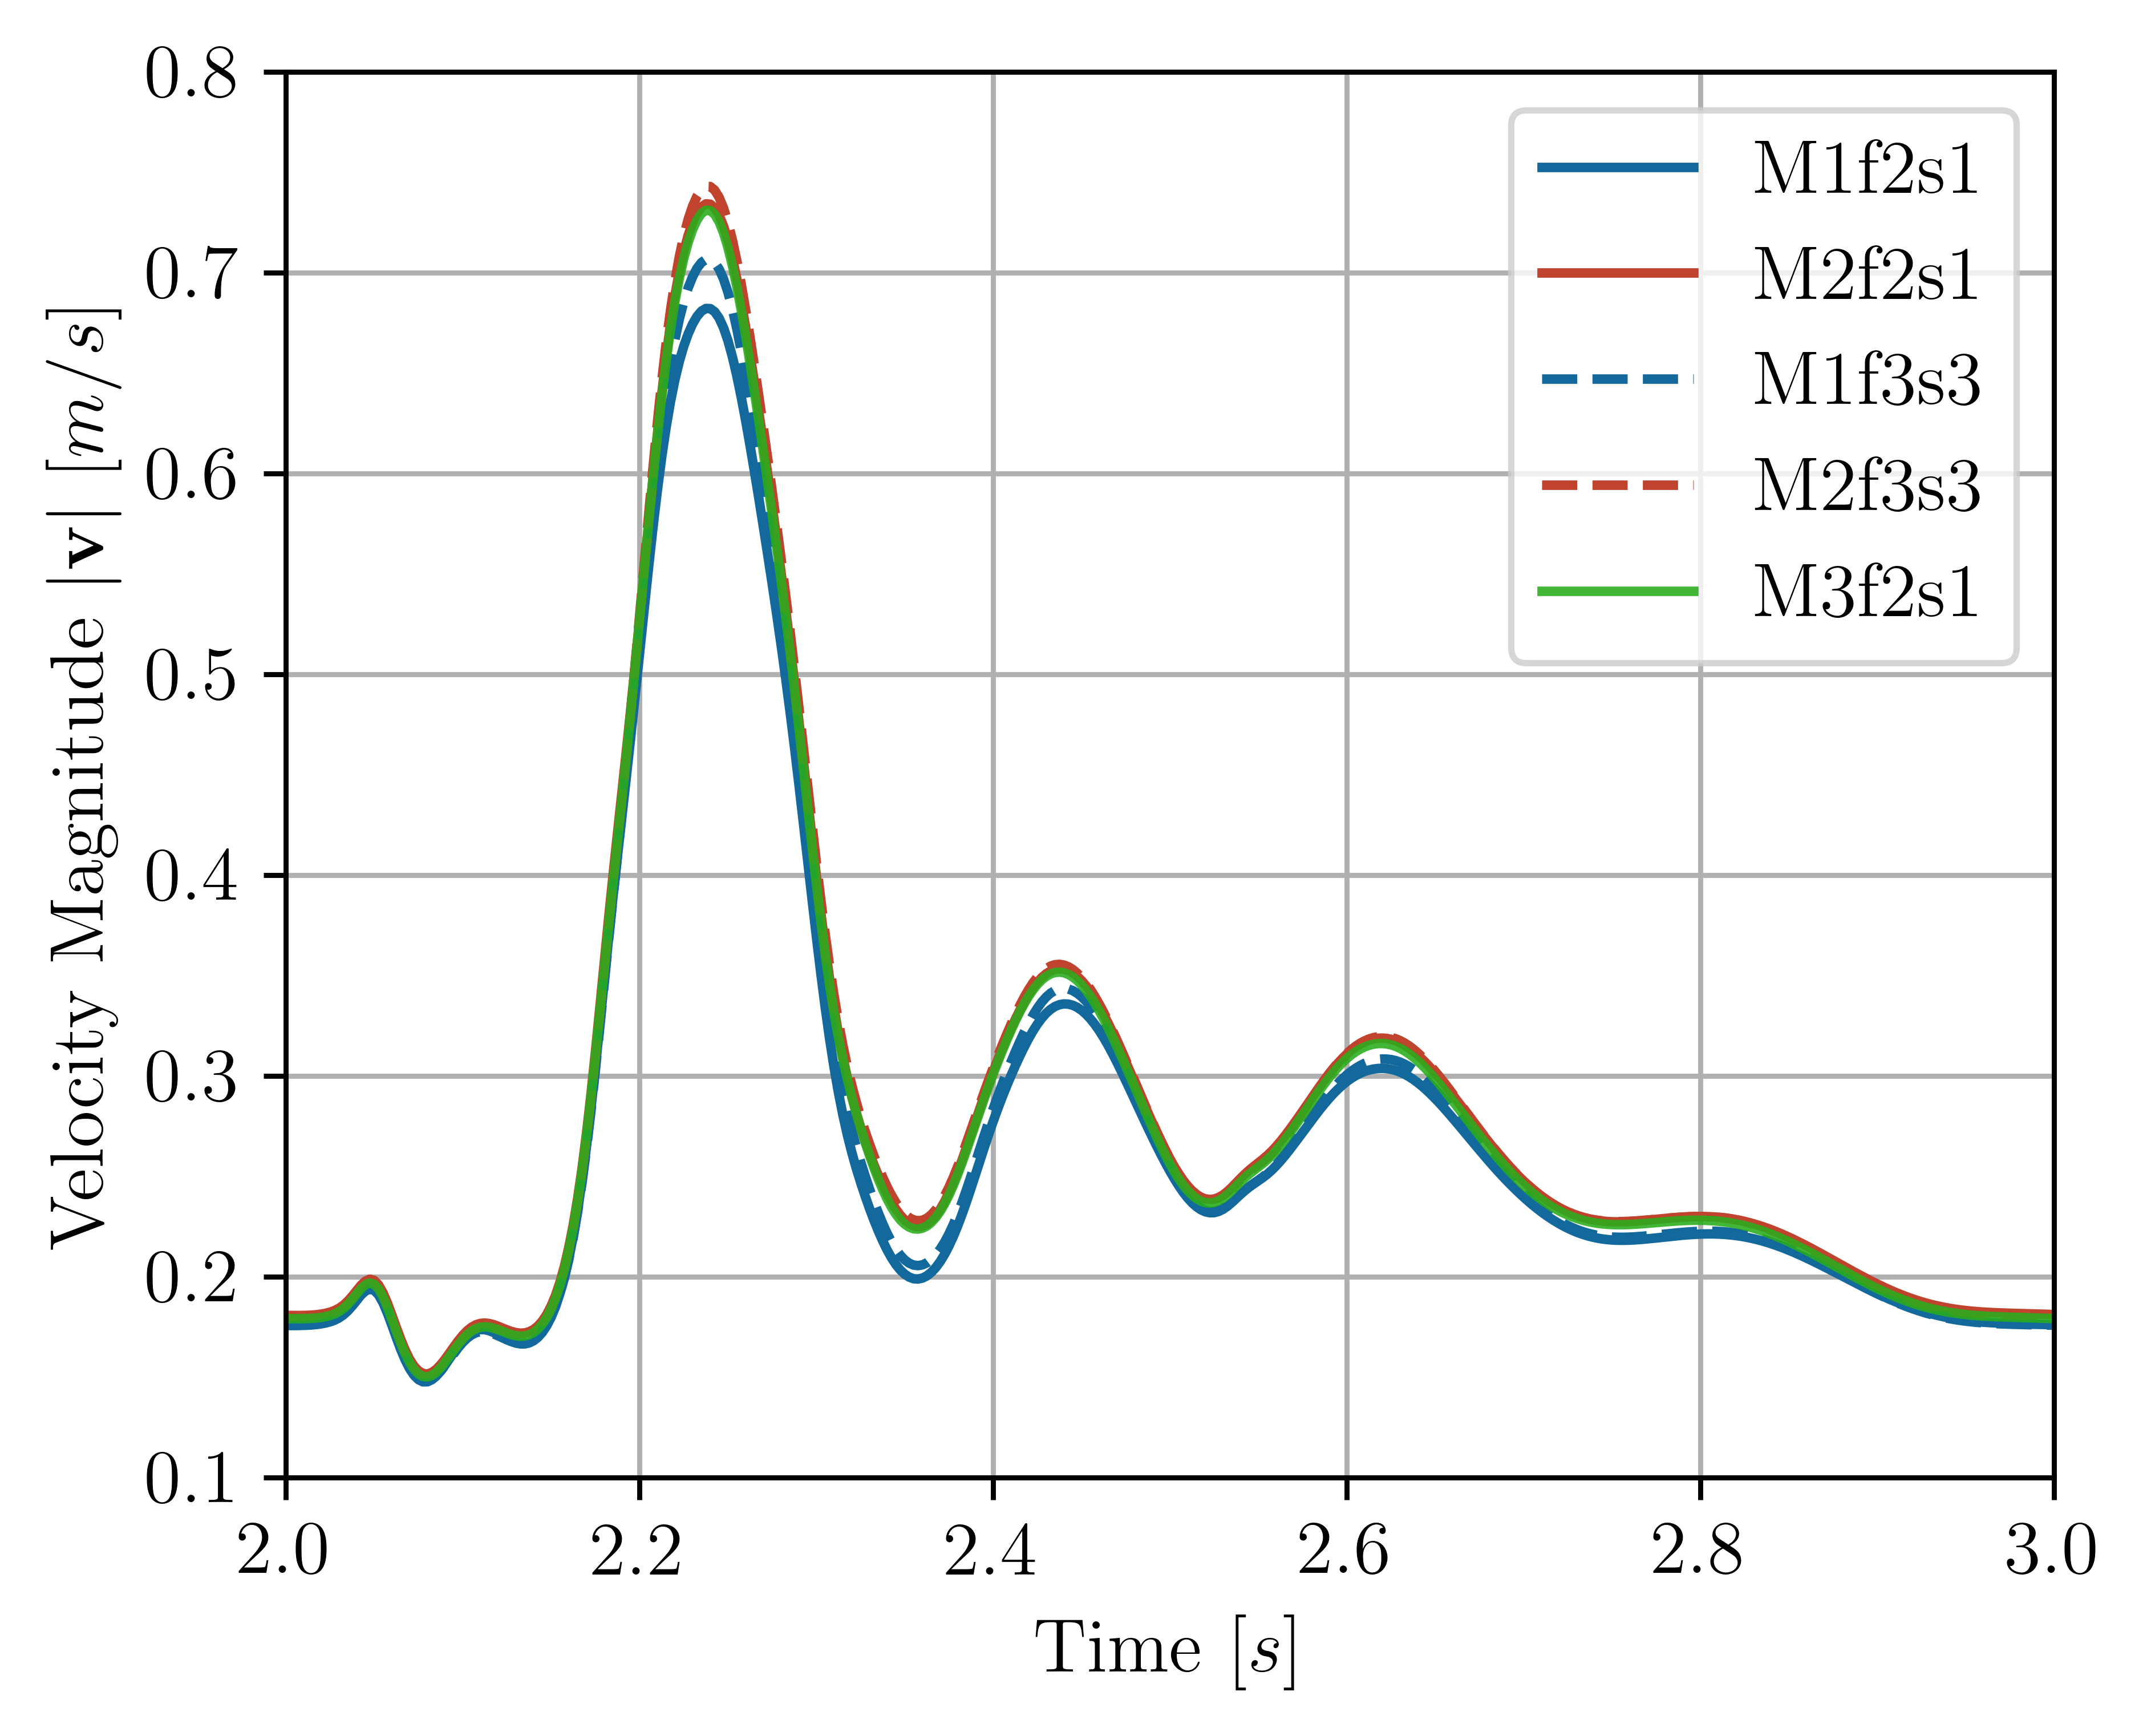
\includegraphics[width=0.475\linewidth]{Figures_carotide/Velocity_Magnitude_punto_wall.png}
    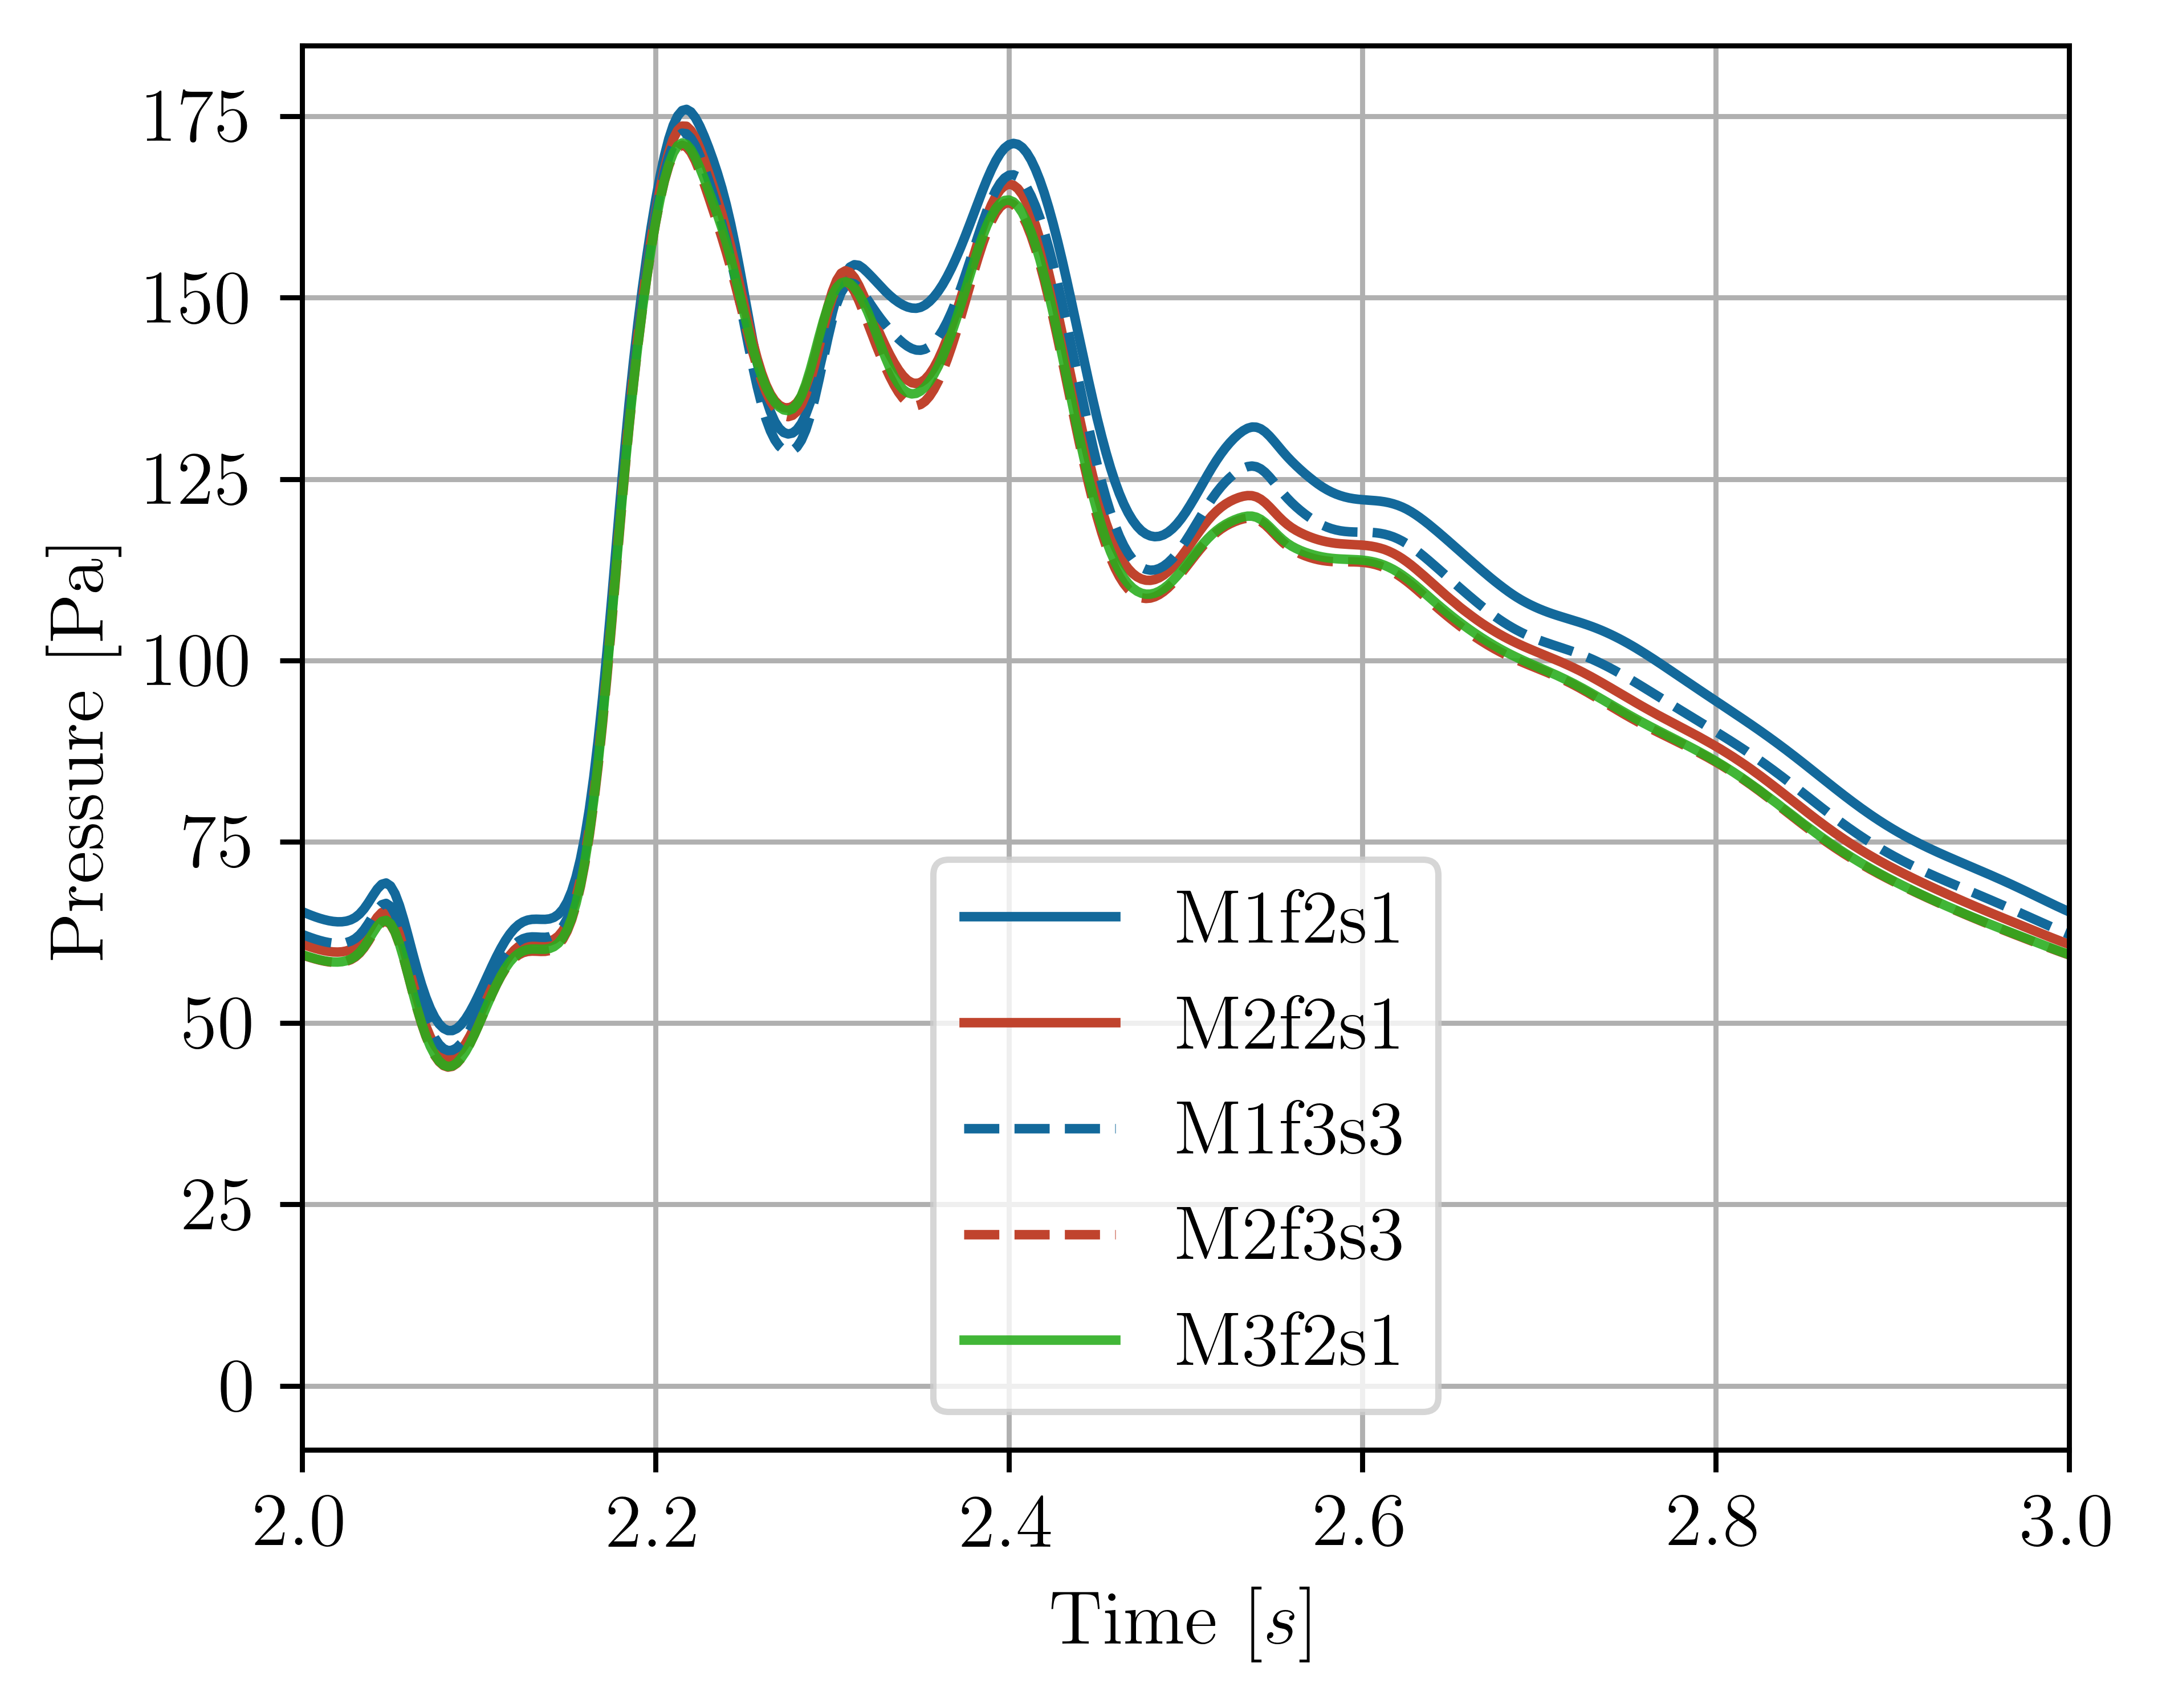
\includegraphics[width=0.475\linewidth]{Figures_carotide/Pressure_Magnitude_punto_wall.png}
    \caption{Carotid blood flow. Mesh comparison at point $p^{\text{wall}}_{\text{CCA}}$.}
    \label{fig:placeholder}
\end{figure}

\subsubsection{Results and comparison}
First, we show the time-averaged velocity and pressure distributions in a cross-sectional view of the simulated arterial bifurcation (Fig.~\ref{fig:carotide_velocity_pressure_distribution}). \textcolor{blue}{These results are represented on the reference configuration, as the time averaging was applied to the fluid variables only, not to the moving ALE domain, similarly performed by Lopes et al. (2019) \cite{lopes2019}}.

Although three different settings were analyzed, only one is displayed here, as the results for all cases exhibit highly similar profiles. This similarity arises from the fact that, in our formulations, both velocity and pressure are treated as unknowns in the fluid problem.
\begin{figure}[h!]
    \centering
    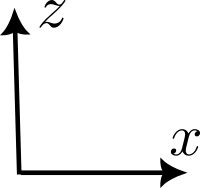
\includegraphics[width=0.07\linewidth]{Figures_carotide/sinus_axes.png}
    \subfloat[Velocity distribution.]{
    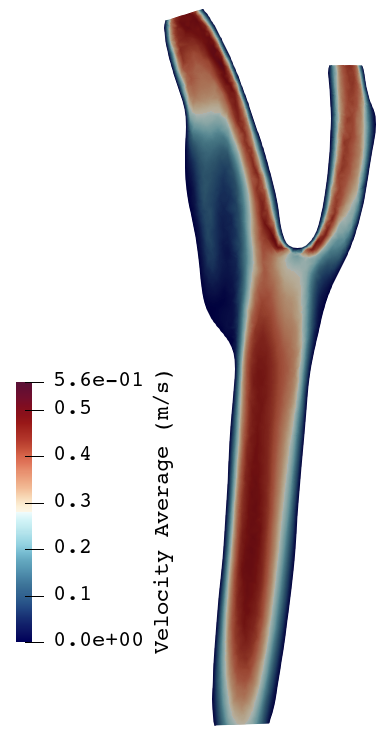
\includegraphics[width=0.3\linewidth]{Figures_carotide/Carotid_vel_av_3cycles.png}}
    \subfloat[Pressure distribution.]{
    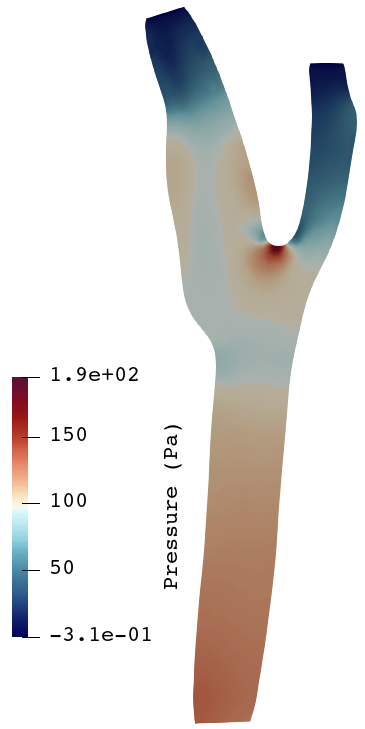
\includegraphics[width=0.29\linewidth]{Figures_carotide/Carotid_press_av_3cycles.png}}
    \caption{\textcolor{blue}{Carotid blood flow. Time-averaged flow distribution in a cross-sectional view, represented in the reference configuration domain.}}
    \label{fig:carotide_velocity_pressure_distribution}
\end{figure}
On the one hand, the velocity profile exhibits the expected characteristics of a flow within a bifurcating artery. Higher velocity magnitudes are concentrated in the central region of the vessel, while near the arterial walls, the velocity decreases. A significant reduction in velocity is observed within the widened section of the internal carotid artery, likely due to flow deceleration and local recirculation. On the other hand, the pressure distribution highlights a smooth pressure gradient along the main arterial segment, with higher values upstream and a noticeable drop near the bifurcation. The pressure reaches a maximum of approximately 190 Pa in average, with a pronounced reduction occurring at the carotid sinus, a region known for flow disturbances and altered WSS. This drop in pressure is indicative of energy dissipation and potential flow separation in this region. These results align with the expected hemodynamic behavior of arterial bifurcations, where complex flow interactions significantly influence local shear forces and vascular remodeling \cite{kaid2024unveiling}.
Moreover, the temporal evolution of velocity and pressure at the points labeled $p_{\text{CCA}}$, $p_{\text{ICA}}$, and $p_{\text{ECA}}$ (see Fig.~\ref{fig:carotide_fulldomain}) is shown in Fig.~\ref{fig:carotide_velocity_pressure_profiles}. 
\begin{figure}[h!]
    \centering
    \subfloat[Velocity profile evolution over time.]{
    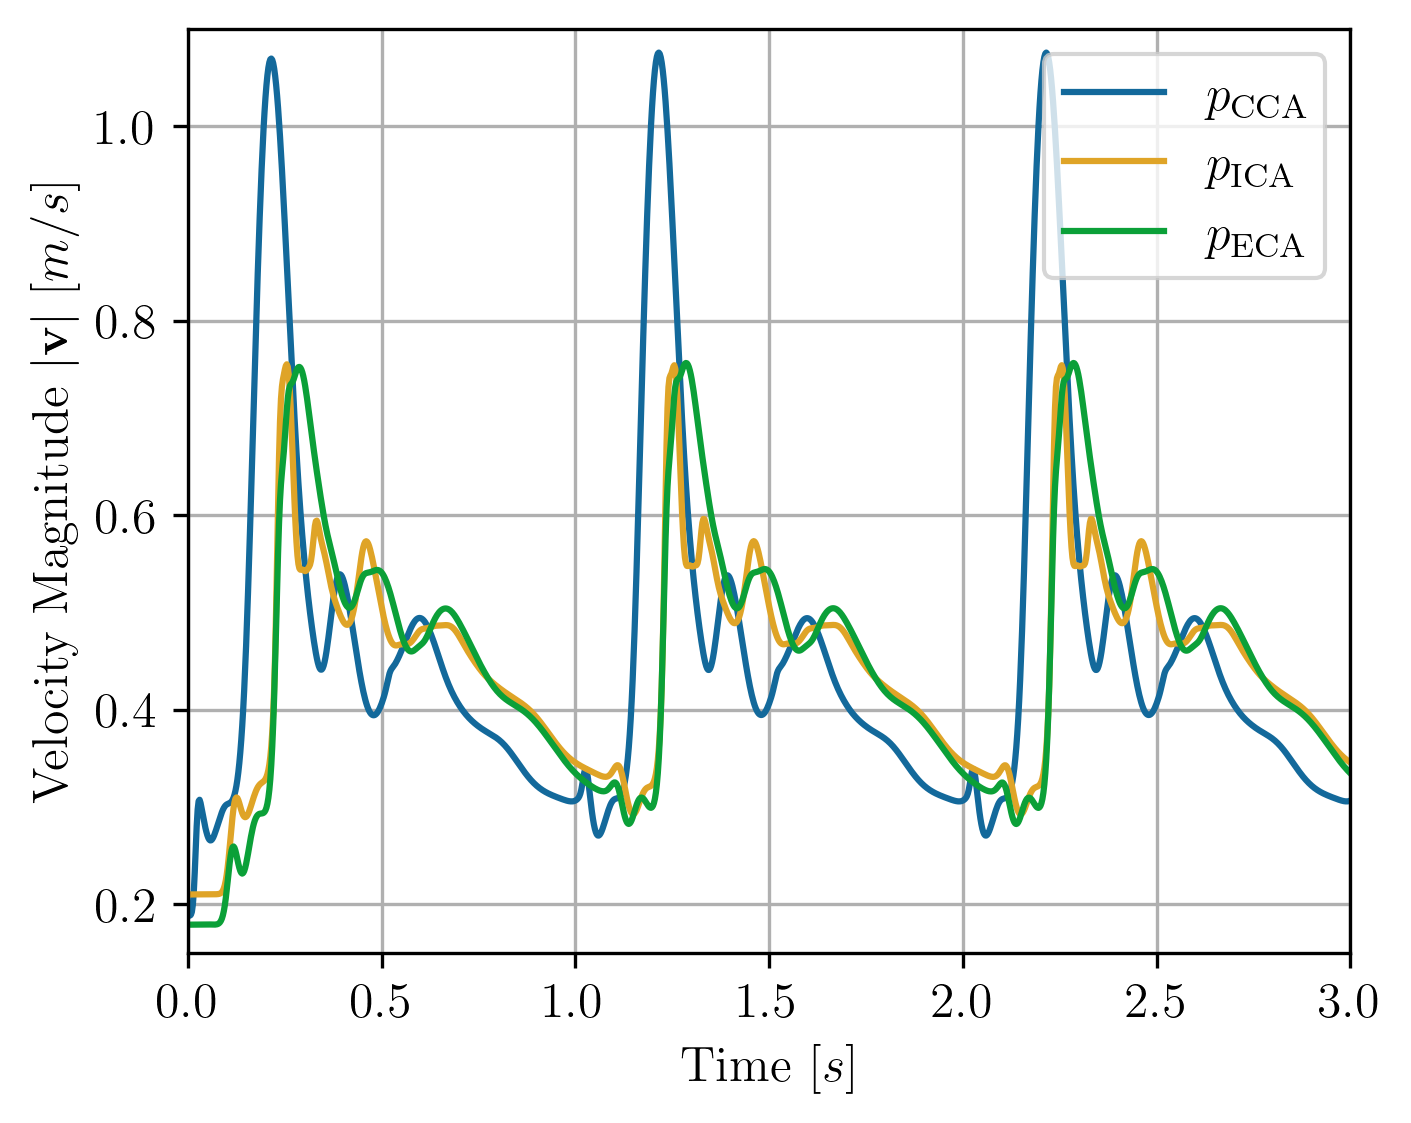
\includegraphics[width=0.475\linewidth]{Figures_carotide/output_velocity_3cycles.png}}
    \subfloat[Pressure profile evolution over time.]{
    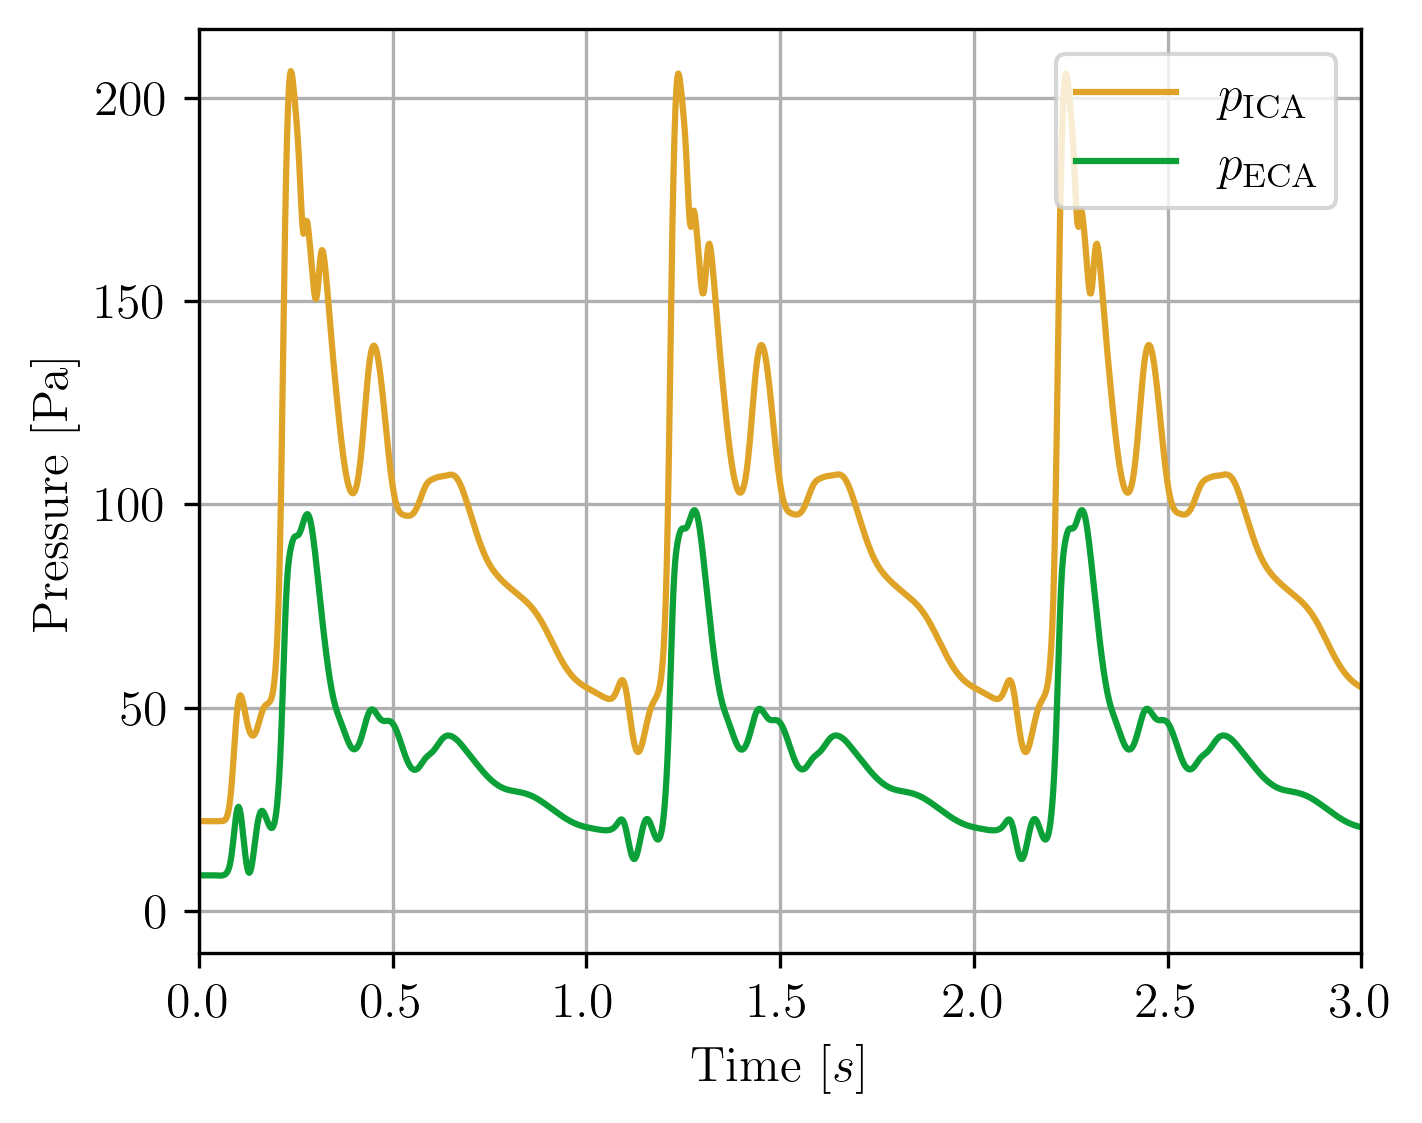
\includegraphics[width=0.475\linewidth]{Figures_carotide/output_pressure_3cycles.png}}
    \caption{Carotid blood flow. Temporal evolution of velocity and pressure profiles near the inlet and outlet regions.}
    \label{fig:carotide_velocity_pressure_profiles}
\end{figure}
While the velocity evolution at the carotid inlet (point $p_{\text{CCA}}$) shows good agreement with \cite{kaid2024unveiling}, the results at the outlets differ from the reference, as does the pressure at both outlets. This discrepancy occurs because we did not prescribe pressure boundary conditions at the outlets in this work. Notably, we observe significant pressure differences between points near the ECA and ICA outlets. The pressure is higher near the ECA outlet due to its significantly smaller diameter compared to the other outlet. Despite these variations, the results remain physically consistent and provide valuable insight into the temporal evolution of velocities, pressures, and subsequent wall shear stress (WSS) patterns.

Next, we analyze WSS distributions in two key hemodynamic regions (see Fig.~\ref{fig:carotide_geometry}): the carotid sinus and apex. Figure~\ref{fig:carotide_sinus_distribution} reveals low WSS zones ($<$0.4~Pa) in the sinus, a known biomarker for endothelial dysfunction, LDL adhesion \cite{zhang2017correlation}, and atherosclerosis initiation \cite{lv2024low}. 
\begin{figure}[h!]
    \centering
    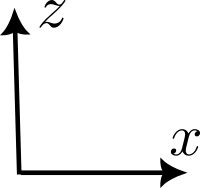
\includegraphics[width=0.07\linewidth]{Figures_carotide/sinus_axes.png}
    \subfloat[M1\_f2s1]{
    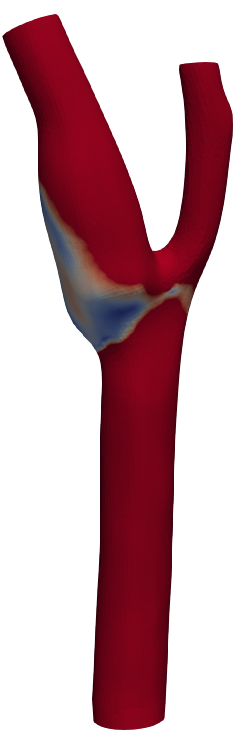
\includegraphics[width=0.17\linewidth]{Figures_carotide/sinus-M1f2s1.png}
    }
    \subfloat[M1\_f3s3]{
    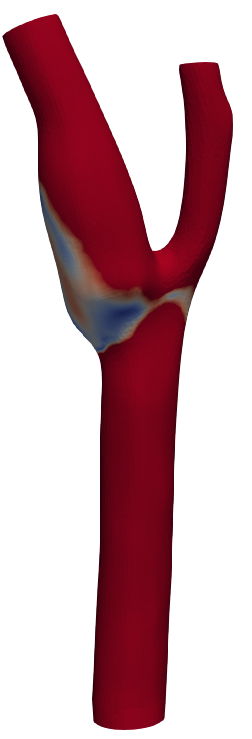
\includegraphics[width=0.17\linewidth]{Figures_carotide/sinus-M1f3s3.png}
    }
     \subfloat[M2\_f2s1]{
    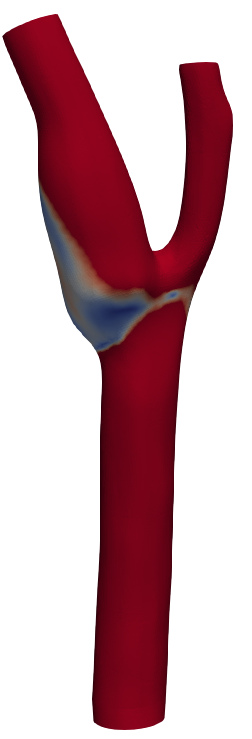
\includegraphics[width=0.17\linewidth]{Figures_carotide/sinus-M2f2s1.png}
    }
    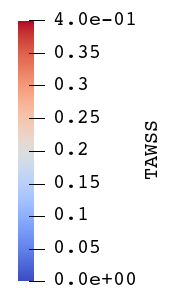
\includegraphics[width=0.17\linewidth]{Figures_carotide/sinus-legend.png}
    \caption{Carotid blood flow. TAWSS distribution on the carotid surface sinus for the three configurations.}
    \label{fig:carotide_sinus_distribution}
\end{figure}
All configurations exhibit the characteristic low-WSS pattern (blue regions), confirming flow recirculation. Moreover, Fig.~\ref{fig:WSS_comparison_carotid_sinus} presents a comparison of the WSS distribution along a selected path, through the carotid sinus, for the three studied configurations (see yellow line in Fig.~\ref{fig:carotide_fulldomain}). This analysis aims to assess the impact of different formulations on the accuracy of WSS computation, particularly in detecting critical shear stress variations along the arterial wall.
\begin{figure}[h!]
    \centering
    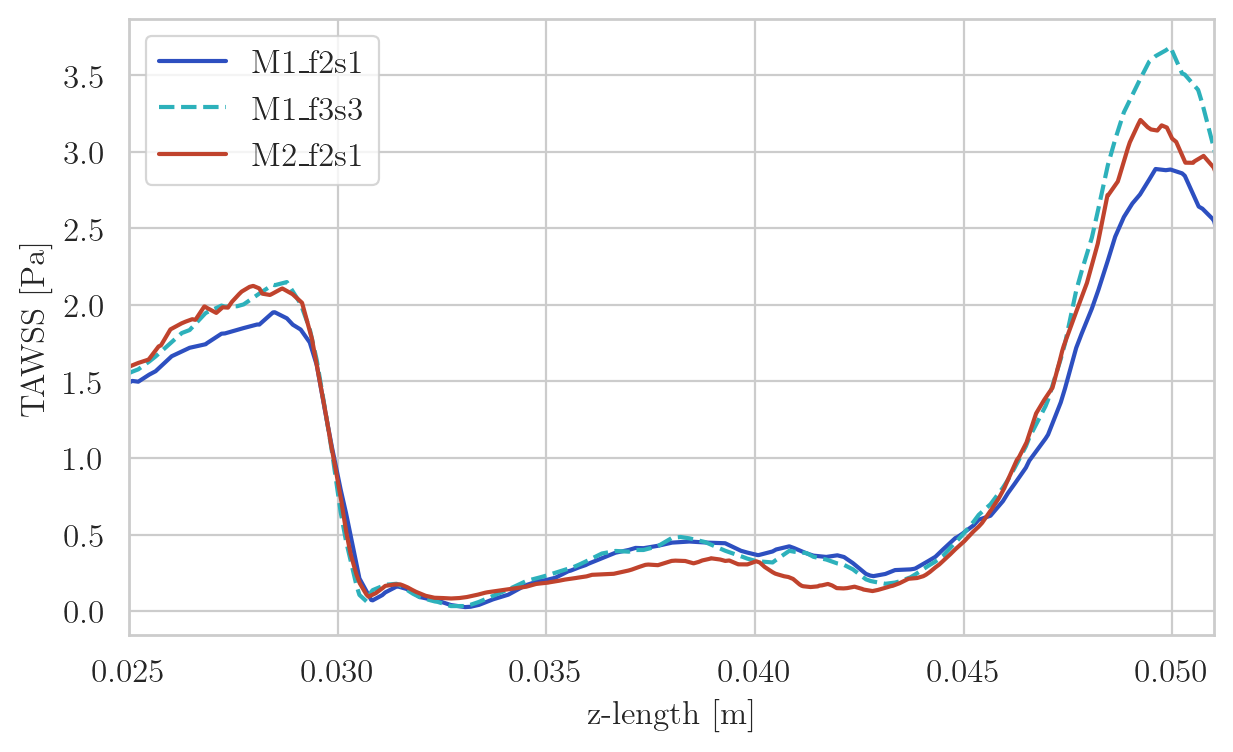
\includegraphics[width=0.65\linewidth]{Figures_carotide/output_sinus-line.png}
    \caption{Carotid blood flow. WSS comparison on the carotid surface sinus.}
    \label{fig:WSS_comparison_carotid_sinus}
\end{figure}
All cases show consistent WSS trends, validating the numerical approach. Key differences emerge in high-gradient regions, such as the carotid sinus, where all models accurately capture the near-zero WSS characteristic of recirculation zones.
% Downstream, M1\_f3s3 resolves the post-sinus WSS peak more sharply, aligning with three-formulation advantages for stress gradients. M1\_f2s1 underestimates the peak (fewer DOFs), while M2\_f2s1 shows smoother transitions, suggesting numerical diffusion. The highest WSS occurs at the ICA entrance, with M1\_f3s3 capturing it most precisely. 
Smoother transitions in M1\_f2s1/M2\_f2s1 indicate underestimated shear forces, critical for predicting endothelial responses and plaque stability \cite{gharabi2016,sanmartin2006influencia}.
\begin{figure}[h!]
    \centering
    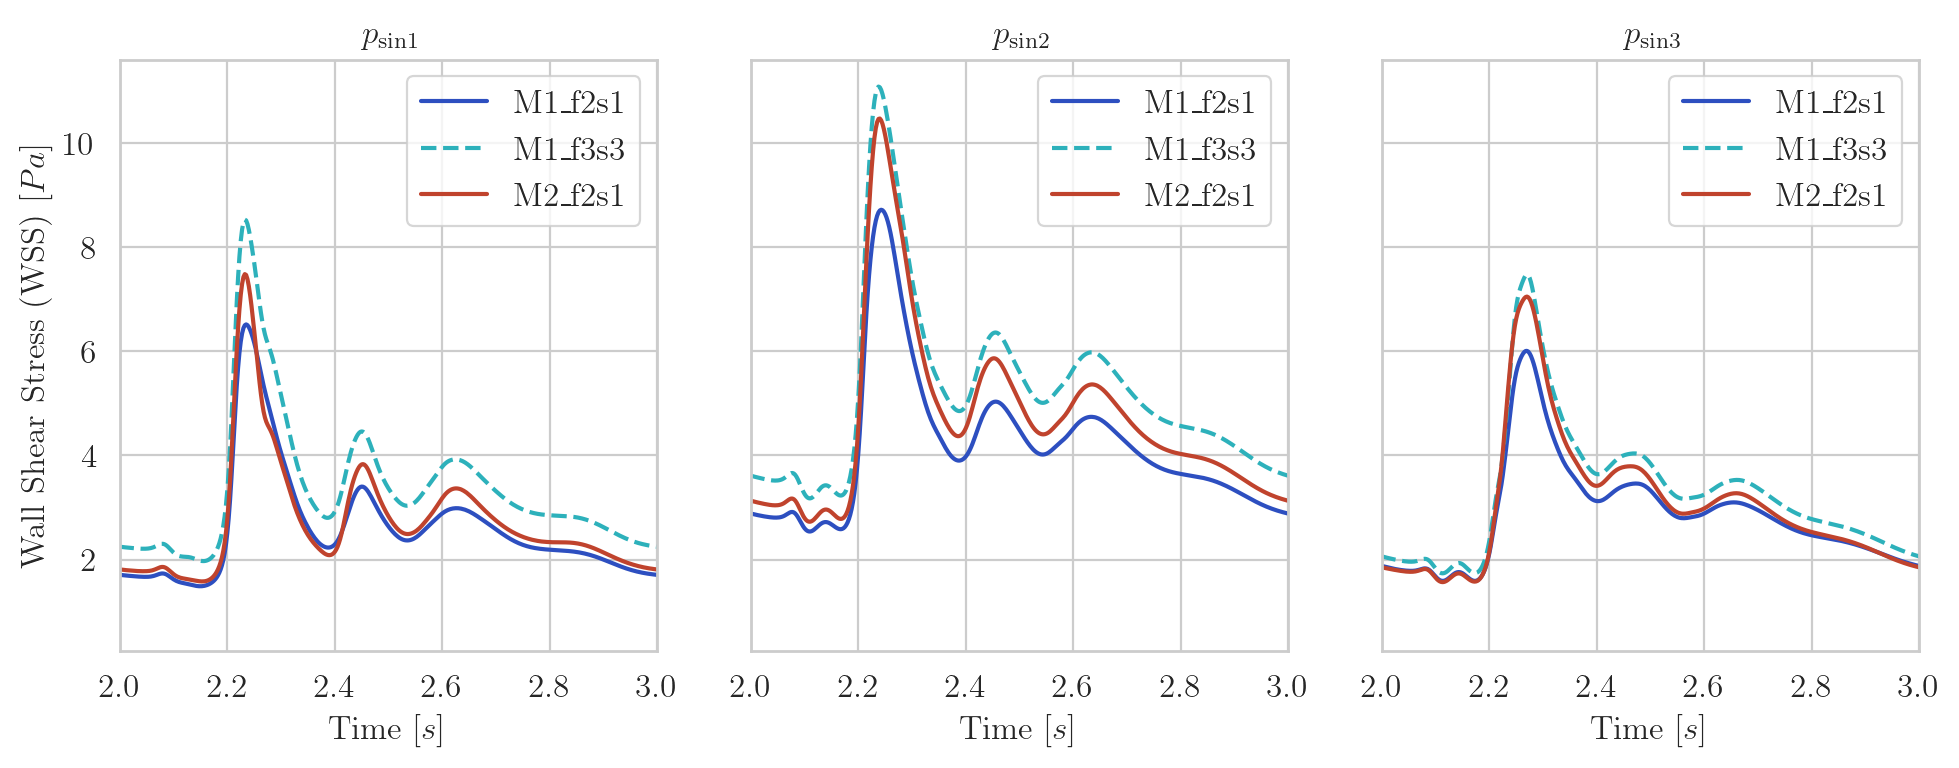
\includegraphics[width=\linewidth]{Figures_carotide/output_sinus-evolution-3cycle.png}
    \caption{Carotid blood flow. Evolution in time of the WSS in points ($p_{sin1}$, $p_{sin2}$ and $p_{sin3}$) located over the sinus region.}
    \label{fig:WSS-evolution}
\end{figure}
Additionally, we analyze the temporal evolution of WSS at three boundary points along the carotid sinus (see Fig.~\ref{fig:carotide_geometry}) for all three configurations. The highest WSS values occur at point $p_{sin2}$, located at the sinus mid-section. Notably, the mixed formulation M1\_f3s3 provides superior solution accuracy compared to other configurations, even outperforming results from the finer mesh M2 when combined with the simpler formulation f2s1.

Next, we analyze the WSS values in the apex of the carotid artery. Fig.~\ref{fig:carotide_apex_distribution} presents the WSS distribution on the carotid surface for the three analyzed configurations, highlighting the regions subjected to the highest shear forces. The results capture the spatial distribution of high WSS regions, which are particularly relevant in the context of arterial remodeling and the potential destabilization of atherosclerotic plaques.
\begin{figure}[h!]
    \centering
     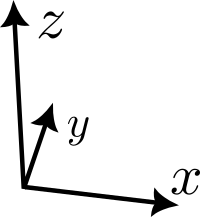
\includegraphics[width=0.07\linewidth]{Figures_carotide/apex_axes.png}
    \subfloat[M1\_f2s1]{
    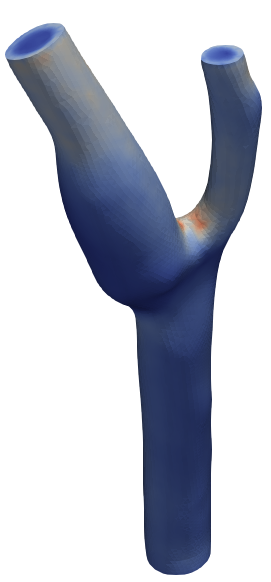
\includegraphics[width=0.2\linewidth]{Figures_carotide/apex-M1f2s1.png}
    }
    \subfloat[M1\_f3s3]{
    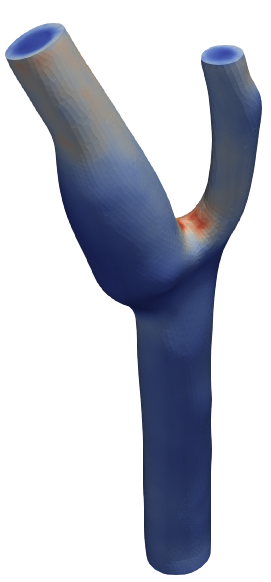
\includegraphics[width=0.2\linewidth]{Figures_carotide/apex-M1f3s3.png}
    }
     \subfloat[M2\_f2s1]{
    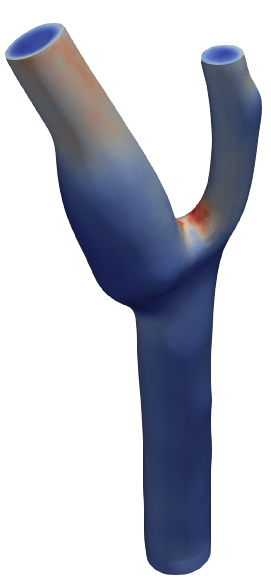
\includegraphics[width=0.2\linewidth]{Figures_carotide/apex-M2f2s1.png}
    }
    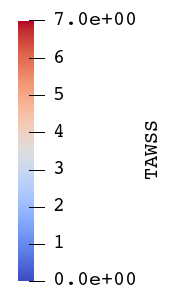
\includegraphics[width=0.17\linewidth]{Figures_carotide/appex-legend.png}
    \caption{Carotid blood flow. TAWSS distribution on the carotid surface for the three configurations.}
    \label{fig:carotide_apex_distribution}
\end{figure}
The highest wall shear stress (WSS) values are concentrated at the bifurcation apex. 
These zones experience strong flow acceleration due to the abrupt geometric changes at the bifurcation, creating steep velocity gradients. As with the sinus analysis, Fig.~\ref{fig:WSS_comparison_carotid_apex} tracks the WSS distribution along a predefined path (red line in Fig.~\ref{fig:carotide_fulldomain}), spanning the bifurcation. This region is hemodynamically critical, as the bifurcation's high WSS directly influences endothelial behavior and plaque stability. The comparison specifically assesses how different numerical formulations (f2s1 vs. f3s3) resolve these shear stress extremes, which are clinically relevant for predicting vascular pathology progression.
\begin{figure}[h!]
    \centering
    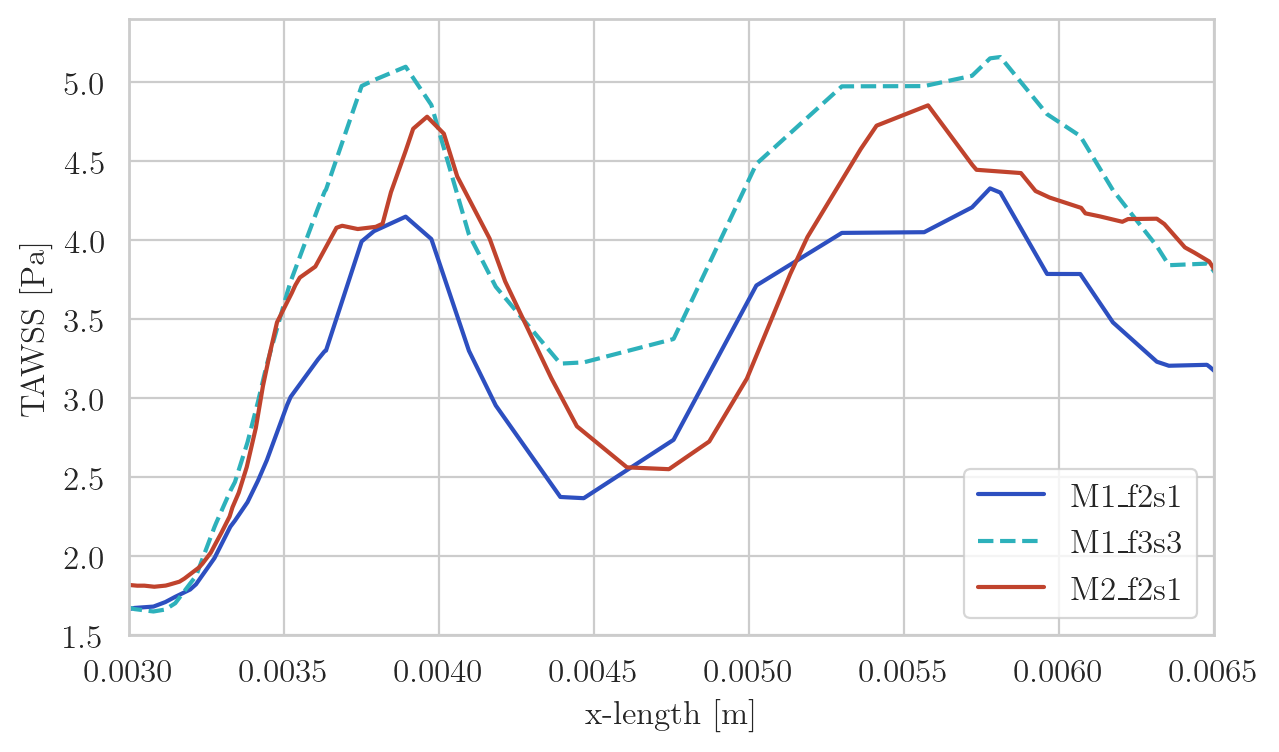
\includegraphics[width=0.65\linewidth]{Figures_carotide/output_apex-line.png}
    \caption{Carotid blood flow. TAWSS comparison on the carotid surface apex.}
    \label{fig:WSS_comparison_carotid_apex}
\end{figure}
Consistent with the sinus analysis, all three cases show similar WSS distributions in this region, though with notable differences in peak localization and gradient resolution. 
While all cases exhibit comparable magnitude peaks, M1\_f3s3 and M2\_f2s1 yield slightly higher values than M1\_f2s1. This suggests the mixed formulation's superior accuracy in stress resolution, whereas the irreducible formulation (M1\_f2s1) likely underestimates shear forces due to reduced DOFs.
The bifurcation apex shows maximum WSS values, with M1\_f3s3 resolving sharper peaks versus the smoother transitions in irreducible formulations.

\begin{figure}[h!]
    \centering
    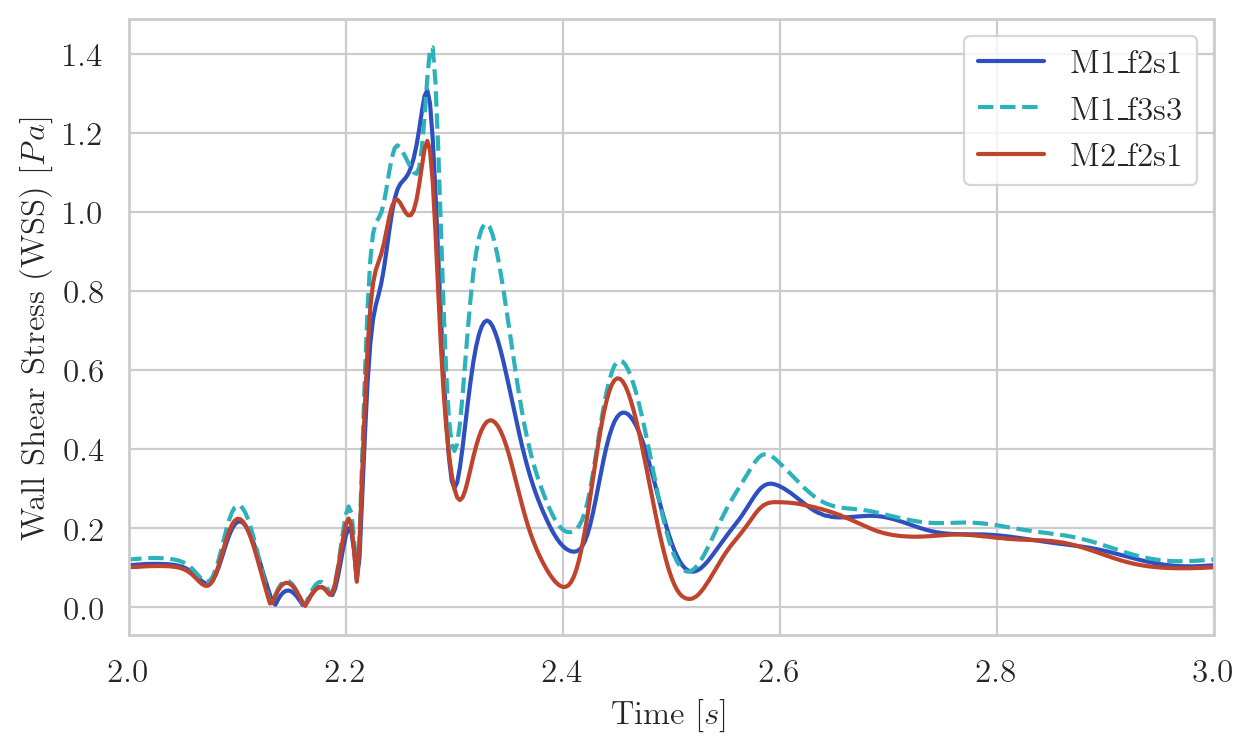
\includegraphics[width=0.65\linewidth]{Figures_carotide/output_apex-evolution-3cycles.png}
    \caption{Carotid blood flow. Evolution in time of the WSS in point $p_{apex}$.}
    \label{fig:WSS-evolution-appex}
\end{figure}
Similar trends are observed in Fig.~\ref{fig:WSS-evolution-appex}, which tracks the WSS temporal evolution at the bifurcation apex. The analysis reveals that the mixed formulation M1\_f3s3 captures the peak WSS magnitude more accurately than other configurations, demonstrating its resolution of high-shear stress gradients in this critical region.

This analysis highlights the advantages of using a mixed three-field formulation for the accurate computation of WSS, particularly in detecting sharp peaks. Since high WSS gradients influence vascular remodeling and disease progression, resolving them with high fidelity is essential for biomechanical modeling. The results demonstrate that the mixed formulation (f3s3) provides improved numerical accuracy compared to the standard irreducible approach (f2s1), while maintaining computational efficiency.
\textcolor{blue}{It should be noted, however, that this example is intended as a numerical benchmark rather than a physiological validation. The plausibility of the results is therefore assessed in terms of numerical stability and physical consistency of the computed fields (pressure, velocity, and wall shear stress), which remain within the typical range reported for laminar arterial flows \cite{hua2015influence}.}

%%%%%%%%%%%%%%%%%%%%%%%%%%%%%%%%%%%%%%%
%
% CONCLUSIONS
%
%%%%%%%%%%%%%%%%%%%%%%%%%%%%%%%%%%%%%%

\section{Conclusions} \label{sec:conclusions}

This study investigates the impact of mixed formulations on FSI problems, focusing on their ability to improve the accuracy and robustness of numerical simulations. By comparing irreducible and mixed formulations in both the fluid and solid domains, we demonstrate the advantages of introducing stress as an additional unknown to enhance the precision of stress-related quantities in different FSI scenarios. From the numerical examples several key conclusions can be drawn regarding the numerical stability, convergence and accuracy of the mixed formulation compared to the irreducible approach. 

First, the results demonstrate that the three-field mixed formulations improve the convergence behavior of the coupled FSI system. In contrast, the irreducible formulations exhibit larger pressure oscillations and require finer mesh resolutions to achieve similar accuracy. This highlights the better numerical stability of mixed formulations, particularly when dealing with incompressible or nearly incompressible materials in the solid domain. 

Second, mixed formulations are shown to be less sensitive to mesh refinement, achieving accurate results even with a coarser mesh. This suggests that introducing stress as an independent unknown enhances the representation of stress fields without significantly increasing computational cost. 

Finally, the results confirm that mixed formulations correctly capture the structural deformation and its interaction with the surrounding fluid, producing smoother and more physically consistent stress distributions. This is particularly relevant for problems where accurate stress transmission at the fluid-solid interface is essential, such as in simulations of flexible structures undergoing large deformations.

These advantages become particularly important in applications requiring high-fidelity stress computations, such as hemodynamic simulations in arterial flows. In these cases, the ability to precisely capture stress variations, especially WSS gradients, plays a crucial role in understanding vascular remodeling, atherosclerosis progression, and plaque stability. The numerical results from our hemodynamic case study confirm that the mixed formulations enhance the resolution of sharp WSS variations, particularly in high-shear regions such as bifurcations and flow reattachment zones, where traditional irreducible methods tend to smooth out peak values, leading to an underestimation of critical stress gradients. The ability of mixed formulations to accurately resolve these stress gradients has direct implications for both biomechanical modeling and clinical applications. These findings highlight the potential of mixed formulations for high-accuracy FSI simulations, paving the way for further research in patient-specific vascular modeling.

\section*{Declaration of competing interest}

The authors declare that they have no known competing financial interests or personal relationships that could have appeared to influence the work reported in this paper.

\section*{Acknowledgements}

R. Codina gratefully acknowledges the support received from the ICREA Acad\`emia Program, from the Catalan Government.
               
%\nocite{*}     
\bibliographystyle{unsrt}
\bibliography{references.bib}

\end{document}
